% Set parameters
% set font size
\documentclass[11pt]{article}

% set line height
\renewcommand{\baselinestretch}{2}

% line number
\usepackage{lineno}

% today
\renewcommand{\today}{}

% set margin
\usepackage{geometry}
\geometry{a4paper, left=15mm, right=15mm, top=20mm, bottom=20mm}

% for using Korean
\usepackage{kotex}

% for using multi-languages
\usepackage[english]{babel}

% for urls
\usepackage{hyperref}

% for equation
\usepackage{amsmath}
\usepackage{mathtools}

% for fixing figure position
\usepackage{float}

% for citation
\usepackage{natbib}
\bibliographystyle{apa}
\setcitestyle{authoryear,open={(},close={)},citesep={;}}

% for drawing table
\usepackage{array,multirow,graphicx,rotating,booktabs}
\usepackage[table,xcdraw]{xcolor}

% for tabularx
\usepackage{tabularx}
\newcolumntype{b}{X}
\newcolumntype{s}{>{\hsize=.5\hsize}X}
\renewcommand\arraystretch{0.8} \setlength\minrowclearance{0.8pt}

% for itemize
\usepackage{enumitem}

%%%%%%%%%%%%%%%%%%%%%%%%%%%%%%%%%%%%%%%%%%%%%%%%%%%%%%%%%%%%%%%%%%%%%%%%%%%%%%%
\begin{document}
\title{미등록단어 문제와 데이터 부족 현상을 해결하기 위한 비지도학습 토크나이저와 추출 기반 문서 요약 기법\\
Unsupervised Korean Tokenizer and Extractive Document Summarization to Solve Out-of-Vocabulary and Dearth of Data}
\author{김현중}
\maketitle
\smallskip

%%%%%%%%%%%%%%%%%%%%%%%%%%%%%%%%%%%%%%%%%%%%%%%%%%%%%%%%%%%%%%%%%%%%%%%%%%%%%%%
\section{개요} \label{introduction}

자연어처리 (natural language processing) 는 사람의 언어를 컴퓨터가 이용할 수 있는 형태의 정보로 변환하고, 이를 이용하여 과업들 (tasks) 을 수행하는 분야이다.
자연어처리에서 수행하는 과업은 다양하다.
품사 판별과 형태소 분석은 텍스트를 단어열로 분해하는 전처리 과업에 해당한다.
단어의 특정 품사나 의미를 이해하는 객체명 인식과, 키워드나 핵심 문장을 이용하여 문서 집합을 요약하는 정보 추출 과업도 자연어처리에 포함된다.
또한 사용자의 질문에 대해 적절한 답변을 탐색하는 질의 응답도 자연어처리 과업에 포함된다.

자연어처리 과업의 많은 부분은 머신러닝 기법을 이용한다.
머신러닝은 학습 방식에 따라 세 가지로 분류할 수 있다.
지도기반 (supervised) 머신러닝은 객체의 특징을 기술하는 입력값 (input) 과 객체의 정답인 출력값 (output) 이 쌍으로 존재할 때 이를 이용하는 방식이다.
머신러닝 모델은 입력값으로부터 출력값을 예측하기에 유용한 정보를 학습한다.
품사 판별의 경우, 단어 - 품사 쌍으로 이뤄진 학습 데이터를 이용하여, 단어열이 입력되었을 때 이에 해당하는 품사열을 판별하는 정보를 모델이 학습한다.
이후, 새로운 단어열이 입력되면 적절한 품사열을 출력한다.
비지도기반 (unsupervised) 머신러닝은 데이터에 입력값만 존재할 때 쓰는 방법으로, 품사 판별의 경우, 두 단어가 앞 뒤에 등장하는 단어들의 분포가 비슷하면 하나의 품사로 이를 인식하는 Brown clustering \citep{brown1992class} 방법이 이에 해당한다.
강화학습 (reinforcement learning) 은 각 입력값에 대한 출력값은 주어지지 않았지만, 출력값에 대한 리워드 (reward) 를 정의할 수 있을 때 이용하는 방식이다.
출력값에 대하여 피드백을 줄 수 있는 도메인에서 이용할 수 있다.
대화 시스템에서 출력된 답변에 대한 피드백을 이용하여 답변 출력 방법을 수정하는 모델이 이에 해당한다 \citep{mo2018personalizing, singh2000reinforcement, li2016deep}. 

많은 자연어처리 연구들은 지도기반 머신러닝을 이용한다.
입력값과 출력값으로 구성된 학습 데이터를 구축한 뒤, 지도기반 모델을 이용하여 입력값과 출력값의 관계를 학습한다.
품사 판별의 경우, 단어 - 품사 쌍으로 이뤄진 말뭉치를 이용하여 한 단어의 앞 뒤에 등장하는 문맥들을 고려하여 해당 단어의 품사를 추정하는 판별 모델을 학습한다.
품사 판별과 같은 과업은 텍스트 데이터를 벡터로 변환하는 전처리 과정에 이용되며, 강화학습처럼 결과값에 대한 피드백을 정의하기가 어렵기 때문에 지도기반 머신러닝 방법이 이용된다.

그러나 지도기반 머신러닝 방법을 이용하는 자연어처리 모델들은 공통적으로 다음과 같은 어려움이 있다.

\begin{enumerate}[noitemsep]
    \item \textbf{Out of vocabulary problem} : 학습 데이터에 등장하지 않은 단어를 제대로 인식하지 못하는 문제이다.
    \item \textbf{Dearth of Data} : 과업에 적합한 학습 데이터를 마련하기 어렵다.
    \item \textbf{Error in data} : 띄어쓰기 오류 및 철자법 오류는 잘못된 자연어처리 과업 결과를 야기한다.
\end{enumerate}

첫째, 미등록단어 문제는 학습 데이터를 이용하는 지도기반 머신러닝 방법에서는 필연적으로 발생하는 문제이다.
언어는 사용되는 시기와 도메인에 따라 다르기 때문에 한 종류의 학습 데이터에 모든 종류의 단어가 등장하지 않는다.
특히 품사 판별기와 같은 전처리 과업에서 자주 발생하는 문제로, 신조어와 같이 새롭게 만들어진 단어를 인식하지 못하여 문장이 잘못된 단어열로 분해된다.
이 결과를 이용하면 문장이나 문서를 잘못된 벡터로 표현되기 때문에 이후의 과업들의 성능이 저하된다.
영어와 같은 언어들은 단어를 띄어쓰기로 구분되며, 최근의 단어 임베딩 기법들을 이용하여 품사의 추정이 손쉽게 이뤄진다 \citep{turian2010word, mikolov2013efficient, collobert2011natural}.
단어의 경계가 띄어쓰기로 구분되지 않는 한국어, 중국어, 일본어에서는 미등록단어를 제대로 인식하기 위해서는 추가적인 단어 사전 혹은 학습 데이터가 필요하다.

둘째, 학습 데이터가 존재하지 않거나, 이를 구축하기 어려운 경우들이 많다.
객체명 인식은 장소, 사람과 같이 단어의 의미적 클래스를 분류하는 과업이다.
지도학습 기반으로 객체명 인식 모델을 학습하려면 각 클래스가 태깅된 학습 데이터가 필요하다.
하지만 객체명 인식이 필요한 도메인마다 단어 클래스가 다르기 때문에 새롭게 학습 데이터를 구축해야 한다.
영화 제목을 인식하는 객체명 인식 모델을 학습하기 위해서는 영화 제목이 태깅된 학습 데이터가 필요하며, 뉴스의 정치인 이름을 인식하는 모델을 학습하기 위해서는 정치인 이름이 태깅된 학습 데이터가 필요하다.

셋째, 텍스트 데이터에는 오류가 존재한다.
띄어쓰기와 같은 문법 오류나 잘못된 철자법에 의하여 한 단어가 다른 의미의 단어로 인식될 수 있다.
사람은 텍스트에 일정 수준의 오류가 포함되어 있다 하더라도 가독에 큰 어려움이 없지만, 자연어처리 과업에 이용되는 많은 수의 머신러닝 알고리즘은 오류에 의하여 오작동할 가능성이 크다.
자연어처리 과업의 성능을 높이기 위해서는 노이즈를 제거하는 과정을 거쳐야 하거나, 오류에 강건한 모델을 이용해야 한다.

이 논문에서는 다음의 한국어 자연어처리 과업에서 발생하는 위의 세 가지 문제를 해결하는 방법들을 제안한다.

\begin{enumerate}[noitemsep]
    \item 문장에서 단어를 인식하는 토크나이징 과업
    \item 키워드와 핵심 문장 추출을 통한 문서 집합 요약
\end{enumerate}

이 논문에서는 비지도학습 기반 접근 방법으로 위의 두 가지 자연어처리 과업을 해결하는 방법을 제안한다.
비지도학습 기반 방법은 학습데이터에 대한 의존도가 낮기 때문에 다양한 문제에 적용하기 용이하다.
또한 비지도학습 기반 방법들은 같은 과업을 해결하는 지도학습 기반 방법들을 보완하는 역할을 할 수 있기 때문에 비지도학습 기반 방법의 성능이 향상될수록 지도학습 기반 방법의 성능도 향상시킬 수 있다.

또한 이 논문에서는 한국어의 구조적 특징을 이용하여 위의 과업을 해결하는 방법을 제안한다.
비지도학습 기반 방법은 데이터로부터 학습할 수 있는 통계 정보를 이용한다.
데이터에 대한 가정은 비지도학습 기반 모델의 사전 지식 (prior knowledge) 역할을 하며, 데이터로부터 학습해야 하는 항목을 명확해 지도록 도와준다.
그렇기 때문에 이 논문에서는 한국어의 구조적 특징을 이용하는 비지도학습 기반 접근으로 한국어 자연어처리 과업의 성능을 향상할 수 있는 방법을 제안한다.

토크나이징 과업은 문장을 단어나 형태소열로 인식하는 것으로, 다른 자연어처리 과업의 전처리 과정으로 이용된다.
그렇기 때문에 토크나이저의 품질이 좋지 않으면 이를 이용하는 다른 과업의 품질에도 영향을 미친다.
학습데이터를 이용하는 지도학습 기반 토크나이저는 새로운 단어를 제대로 인식하지 못할 가능성이 높다.

\ref{word_extraction} 장에서는 한국어의 언어 특징을 이용하여 단어 인식 성능을 향상한 비지도학습 기반 한국어 토크나이저를 제안한다.
지도학습 기반 토크나이저의 미등록단어 문제를 해결하기 위하여 단어 추출 방법을 이용하는 비지도학습 기반  토크나이저가 이용될 수 있다.
비지도학습 기반 토크나이저는 통계 정보만을 이용하여 문장에서 단어의 경계를 인식하기 때문에 언어별 특징을 함께 이용할 경우 토크나이저의 품질이 향상될 수 있다.

\ref{noun_extraction} 장에서는 한국어의 언어 특징을 이용한 통계 기반 명사 추출 방법을 제안한다.
토크나이징 과업에서 미등록단어 문제를 해결하는 다른 방법으로 지도학습 기반 토크나이저에 단어 사전을 보강할 수 있다.
한국어에서는 특히 명사에서 미등록단어 문제가 자주 발생하며, 명사는 키워드 추출이나 토픽 모델링과 같은 자연어처리 과업에서 가장 중요한 품사의 단어이기 때문에 정확한 인식이 필요하다.

\ref{summarize_single_topic} 장에서는 그래프 랭킹 알고리즘 기반으로 한국어 문서에서 키워드와 핵심 문장을 선택하는 추출 기반 문서 요약 방법을 제안한다.
문서 요약 과업은 주어진 문서 집합의 주제의 다양성에 따라 접근 방법이 달라진다.
\ref{summarize_single_topic} 장에서는 문서 집합이 단일한 주제로 이뤄진 상황에서 미등록단어 문제를 해결하기 위해 토크나이저를 이용하지 않는 한국어 키워드 추출 방법을 제안한다.
또한 추출된 키워드 집합을 이용하여 중복되지 않는 핵심 문장을 추출하는 방법을 함께 제안한다.

\ref{improved_kmeans} 장에서는 다양한 주제로 구성된 문서 집합을 요약하기 위한 문서 군집화 기반 문서 요약 방법을 제안한다.
효율적인 문서 군집화를 위하여 개선된 spherical k-means 알고리즘을 제안하며, 추가적인 모델 학습 없이 군집화 결과만을 이용하여 군집 별 키워드를 추출할 수 있는 방법을 제안한다.

\ref{related_works} 장에서는 위의 각 장이 해결하는 자연어처리 과업에 공통적으로 이용되는 관련 연구를 정리한다.
이 장은 한국어의 구조와 단어 임베딩 기법, 순차적 판별 알고리즘, 추출 기반 문서 요약 기법으로 구성되어 있다.

%%%%%%%%%%%%%%%%%%%%%%%%%%%%%%%%%%%%%%%%%%%%%%%%%%%%%%%%%%%%%%%%%%%%%%%%%%%%%%%
\newpage
\section{관련 연구} \label{related_works}

\subsection{한국어의 구조}

한국어의 문장은 어절로 구성되어 있으며, 어절은 띄어쓰기를 기준으로 나뉘는 단위이다.
한 어절은 하나의 단어 혹은 여러 개의 단어로 구성될 수 있다.
그리고 단어는 하나 이상의 형태소로 구성된다.
한국어의 단어 품사 종류는 5언 9품사이며, 각 단어는 그 자체로 형태소 품사를 지닌다 (표 \ref{tab:korean_tag}).
단 형용사와 동사는 용언의 어간과 어미 형태소로 구성된다.

"이것은 예문 입니다" 라는 문장은 세 개의 어절로 구성되어 있으며, "이것은" 어절은 "이것/명사 + 은/조사"로 구성된다  (그림 \ref{tab:korean_tag}).
"입니다"는 하나의 단어인 "입니다/형용사"로 구성되어 있는데, 이는 "이/형용사 어간 + ㅂ니다/어미"라는 두 개의 형태소로 구성된다.
"예문"은 하나의 형태소가 하나의 단어를 이루며, 하나의 단어가 하나의 어절을 이룬 경우이다.

\begin{figure}[H]
\centering
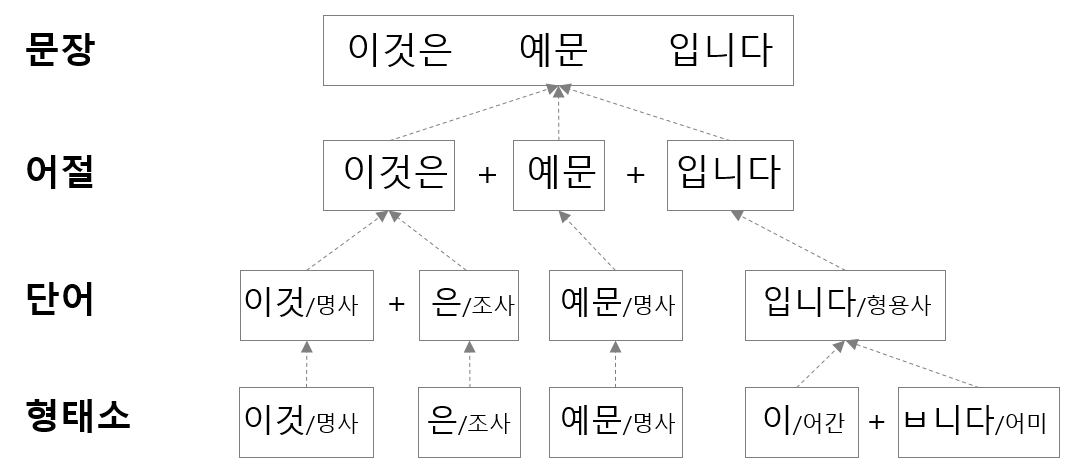
\includegraphics[keepaspectratio=true, width=0.6\linewidth]{figures/korean_structure.png}
\caption{한국어의 문장은 어절로, 어절은 단어로, 단어는 형태소로 구성되어 있다.}
\label{fig:korean_structure}
\end{figure}

단어의 종류는 의미를 지니며 새로운 단어가 만들어지는 열린 집합 (open classes) 과 문법 기능을 수행하며 새로운 단어가 잘 만들어지지 않는 닫힌 집합 (closed classes) 으로 나뉘어진다 \citep{jurafsky2000speech}.
대명사, 관형사, 조사, 어미는 문법 기능을 수행하는 단어와 형태소이기 때문에 닫힌 집합에 해당한다.
체언의 수사도 숫자의 종류가 고정되어 있기 때문에 닫힌 집합에 해당한다.
명사나 감탄사는 새로운 개념을 표현하기 위하여 새로운 단어가 만들어지기 때문에 열린 집합에 해당한다.
동사와 형용사는 명사와 전성어미가 합쳐진 형태로 새로운 어간이 만들어지기 때문에 형태소 수준에서는 닫힌 집합이며, 단어 수준에서는 열린 집합에 해당한다.

\begin{table}[H]
\centering
\begin{tabular}{|
>{\columncolor[HTML]{EAEAEA}}c |
>{\columncolor[HTML]{EFEFEF}}c |c|l|c|c|l|l|}
\hline
\cellcolor[HTML]{EAEAEA} & 체언 & \multicolumn{2}{c|}{명사} & \multicolumn{2}{c|}{대명사} & \multicolumn{2}{l|}{수사} \\ \cline{2-8} 
\cellcolor[HTML]{EAEAEA} & 수식언 & \multicolumn{3}{c|}{관형사} & \multicolumn{3}{c|}{부사} \\ \cline{2-8} 
\cellcolor[HTML]{EAEAEA} & 관계언 & \multicolumn{6}{c|}{조사} \\ \cline{2-8} 
\multirow{-4}{*}{\cellcolor[HTML]{EAEAEA}\textbf{불변어}} & 독립언 & \multicolumn{6}{c|}{감탄사} \\ \hline
\textbf{가변어} & 용언 & \multicolumn{3}{c|}{동사} & \multicolumn{3}{c|}{형용사} \\ \hline
\end{tabular}
\caption{한국어 단어 품사 구조. 한국어는 5언 9품사로 구성되어 있다.}
\label{tab:korean_tag}
\end{table}

%%%%%%%%%%%%%%%%%%%%%%%%%%%%%%%%%%%%%%%%%%%%
\subsection{단어 임베딩 (Word embedding)}

언어 모델 (language model) 은 문장의 생성 확률을 표현하기 위한 방법으로, 식 \ref{eq:slm} 처럼 n-gram 에 기반하여 문장의 확률을 정의할 수 있다 \citep{jurafsky2014speech}.

\begin{equation}
  \label{eq:slm}
  \begin{aligned}
  P(w_{1:p}) = \prod_i P(w_i \vert w_{i-n+1:i-1}) \\
  P(w_i \vert w_{i-n+1:i-1}) = \frac{\#(w_{i-n+1:i})}{\#(w_{i-n+1:i-1)}}
  \end{aligned}
\end{equation}

그러나 n-gram 기반 언어 모델은 n-gram 의 종류가 증가함에 따라 모델의 크기가 기하급수적으로 증가한다.
또한 단어 간 의미적 유사성을 표현하지 못하는 단점이 있다.
이를 해결하기 위하여 피드 포워드 뉴럴 네트워크 기반 언어 모델이 제안되었다 \citep{bengio2003neural}.
\citep{bengio2003neural} 의 언어 모델은 각 단어를 고정된 크기의 임베딩 벡터로 표현한 뒤, $w_{i-n-1:i-1}$ 단어의 벡터를 연결한 입력값으로 $w_i$ 단어를 예측하는 2 층 피드 포워드 뉴럴 네트워크를 제안하였다 (식 \ref{eq:nlm}).

\begin{equation}
  \label{eq:nlm}
  \begin{aligned}
  y = b + Wx + U \cdot tanh(d + Hx) \\
  x = (C(w_{i-n+1}), \dots, C(w_{i-1})), y = w_i
  \end{aligned}
\end{equation}

그 결과 \ref{eq:nlm} 모델은 비슷한 문맥에서 등장하는 단어를 비슷한 벡터로 학습하였다.
하지만 식 \ref{eq:nlm} 의 모델은 오랜 학습 시간이 필요하였다.
\citep{mikolov2013efficient} 는 식 \ref{eq:nlm} 의 입력값과 출력값의 벡터 크기를 동일하게 만들기 위하여 $n-1$ 개 단어의 벡터값의 평균을 입력값으로 변환하여 $w_i$ 를 예측하는 softmax regression 기반 모델인 Word2Vec 을 제안하였다.
피드 포워드 뉴럴 네트워크 기반 언어 모델은 한 단어의 앞에 등장한 단어만 입력값으로 이용하였는데, Word2Vec 은 뒤에 등장한 문맥도 고려하기 위하여 한 단어의 앞 뒤에 등장하는 $w$ 개의 단어의 임베딩 벡터의 평균을 입력값으로 이용한다 (식 \ref{eq:word2vec}).

\begin{equation}
  \label{eq:word2vec}
  \begin{aligned}
  P(w_i \vert w_c) = \frac{exp(w_i^T w_c)}{\sum_j exp(w_j^T w_c)} \\
  w_c = avg(w_{i-w}, \dots, w_{i-1}, w_{i+1}, \dots, w_{i+w})
  \end{aligned}
\end{equation}

또한 클래스의 개수가 단어 개수인 softmax regression 의 학습을 효율적으로 하기 위하여 Noise Contrastive Estimation \citep{gutmann2010noise} 에 기반한 negative sampling 기법을 적용하였다 \citep{mikolov2013distributed}.
그 결과 뉴럴 네트워크 기반 언어 모델처럼 단어의 의미적 정보가 보존된 임베딩 벡터를 빠른 시간 내에 학습할 수 있게 되었다.

GloVe 는 두 단어의 임베딩 벡터를 이용하여 두 단어가 $w$ 간격 안에 함께 등장할 빈도수 $X_{i,j}$ 를 직접 예측하는 regression 문제로 단어 임베딩 벡터를 학습한다 \citep{pennington2014glove}.
식 \ref{eq:glove} 처럼 두 단어 $i, j$ 의 임베딩 벡터 $w_i, w_j$ 의 내적에 bias $b_i, b_j$ 를 더한 값이 co-occurrence 의 로그값 $log(X_{i,j})$ 에 가까워지도록 $w, b$ 를 학습한다.
자주 등장한 단어에 대하여 임베딩 벡터가 더 잘 학습되도록 증가함수 $f(X_{i,j})$ 를 이용하여 각 단어의 손실양에 가중치를 더한다.

\begin{equation}
  \label{eq:glove}
  minimize \sum f(X_{i,j}) \cdot \left( w_i^t w_j + b_i + b_j - log(X_{i,j}) \right)^2
\end{equation}

Word2Vec 과 GloVe 는 \citep{harris1954distributional} 의 "비슷한 의미를 지닌 단어는 비슷한 문맥에서 등장한다"는 가정을 기반으로 임베딩 벡터를 학습한다 .
Word2Vec 은 softmax regression 을 이용하여 비슷한 문맥 (비슷한 입력값)을 지니는 두 단어가 비슷한 임베딩 벡터가 되도록 학습한다.
GloVe 는 단어 $j$ 의 인덱스를 고정할 경우 단어 $i$ 에 대한 선형 회귀식이 되며, 비슷한 문맥에서 등장한 단어는 비슷한 회귀 계수를 지니게 된다.
그리고 Word2Vec 과 GloVe 는 비슷한 단어 임베딩 벡터를 학습한다고 알려졌다 \citep{levy2015improving}

또한 negative sampling 을 이용하는 Word2Vec 의 한 종류인 Skip-gram (SGNS) 은 단어 간 co-occurrence 행렬에 Shifted PMI 를 적용한 공간과 같음이 증명되었다 \citep{levy2014neural}.
식 \ref{eq:levy_pmisvd} 의 $\vec{c}, \vec{w}$ 는 SGNS 의 문맥 단어와 기준 단어의 임베딩 벡터이며, 이들의 내적은 두 단어의 co-occurrnce 의 PMI 값에서 negative samples 의 개수인 $k$ 의 로그값을 뺀 것과 동치임이 증명되었다.
한 단어는 문맥 단어와의 co-occurrence matrix 에 Shifted PMI 를 적용한 벡터로 표현할 수 있다 \citep{levy2014neural}.

\begin{equation}
  \label{eq:levy_pmisvd}
  \vec{w} \cdot \vec{c} = log \left( \frac{\#(w,c) \cdot \vert D \vert}{\#(w) \cdot \#(c)} \cdot \frac{1}{k} \right) = log \left( \frac{\#(w,c) \cdot \vert D \vert}{\#(w) \cdot \#(c)} \right) - log k
\end{equation}

Word2Vec 과 같은 distributed representation 으로 이를 표현하기 위해서 SVD 를 적용할 수 있는데, 식 \ref{eq:better_svd} 처럼 고유값 (eigen value) 행렬을 단어와 문맥 행렬에 나눠 곱해야 SGNS 과 비슷한 단어 임베딩 벡터 $W^{SVD}$ 를 얻을 수 있다 \citep{levy2015improving}.

\begin{equation}
  \label{eq:better_svd}
  \begin{aligned}
  M_d = U_d \cdot \Sigma_d \cdot V_d^T \\
  W^{SVD} = U_d \cdot \Sigma_d^{0.5} \\
  C^{SVD} = V_d \cdot \Sigma_d^{0.5}
  \end{aligned}
\end{equation}


그러나 Word2Vec, GloVe, PMI+SVD 와 같은 단어 임베딩 방법은 빈도수가 작은 단어나 학습 데이터에 등장하지 않은 단어에 대해서는 단어 임베딩 벡터를 얻기가 어렵다.
FastText 는 빈도수가 적은 단어와 미등록단어의 임베딩 벡터를 표현하기 위하여 한 단어를 구성하는 부분단어 (subwords) 의 임베딩 벡터의 합으로 단어 벡터를 표현한다 \citep{bojanowski2017enriching}.
예를 들어 'where' 라는 단어의 임베딩 벡터는 단어의 경계를 표현하기 위하여 단어 앞 뒤에 (, ) 를 추가한 뒤, '(where)' 의 3 \~ 6 글자의 부분단어인 '(wh, whe, ..., where)' 의 임베딩 벡터를 학습한다.
그 뒤 단어 'where' 의 단어의 벡터는 이를 구성하는 모든 부분단어 벡터의 합으로 표현한다.
그 뒤 SGNS 를 이용하여 각 단어를 구성하는 부분단어의 벡터를 학습한다.
그 결과 비슷한 문맥에서 이용되는 부분단어는 비슷한 임베딩 벡터로 표현되며, 형태가 비슷한 단어는 비슷한 부분단어들로 구성되기 때문에 비슷한 임베딩 벡터로 표현된다.

이러한 단어 임베딩 벡터는 이후 다른 자연어처리 과업의 pre-trained 된 벡터로 이용되며, 미등록단어 문제를 해결하기도 한다.
한 문서 집합의 모든 단어를 이용하여 임베딩 벡터를 학습한 뒤 품사 정보가 태깅된 일부 단어를 이용하여 뉴럴 네트워크 기반 품사 판별기를 학습하면 품사 정보가 없는 단어에 대해서 비슷한 임베딩 벡터를 지니는 단어로 품사 태깅이 가능하다.

또한 단어 임베딩 벡터는 각 과업에 따라 단어 벡터가 변할 수 있다.
앞의 단어 임베딩 방법을 이용하면 'good' 과 'bad' 는 비슷한 문맥에서 등장하기 때문에 비슷한 벡터로 학습되지만, 감성 분삭 과업에 의하여 fine-tune 을 하면 서로 다른 벡터로 변환된다 \citep{kim2014convolutional, joulin2016bag}.

그러나 단어 임베딩에서도 미등록단어 문제가 발생한다.
Word2Vec 이나 GloVe 와 같은 단어 임베딩 방법은 학습 과정에 등장하지 않은 단어는 벡터로 표현할 수 없다.
FastText 는 새로운 단어에 대하여 부분단어의 벡터의 합으로 벡터 표현의 추정이 가능하지만, 이는 단어의 형태적 유사성을 바탕으로한 단어 벡터의 추정이며 새로운 문맥적에서 등장하는 단어의 의미는 제대로 표현하지 못한다.

%%%%%%%%%%%%%%%%%%%%%%%%%%%%%%%%%%%%%%%%%%%%
\subsection{순차적 레이블링 (Sequential labeling)}

순차적 레이블링 기법은 길이가 $n$ 인 입력 시퀀스 $x = [x_1, x_2, \dots, x_n]$ 에 대하여 가장 적절한 출력 시퀀스 $y = [y_1, y_2, \dots, y_n]$ 을 출력하는 머신러닝 알고리즘이다 (식 \ref{eq:sequential_labeling}).

\begin{equation}
  \label{eq:sequential_labeling}
  \arg \max_y P(y \vert x)
\end{equation}

식 \ref{eq:sequential_labeling} 를 정의하는 방법에 따라 다양한 순차적 레이블링 기법이 제안되었다.
Hidden Markov Model (HMM) 은 Markov property 를 이용하는 방법으로, 오래전부터 이 문제를 위하여 이용되었다 \citep{krogh1994hidden}.
HMM 은 식 \ref{eq:hmm} 처럼 두 종류의 패러매터로 구성되어 있다.
$P(y_i \vert y_{i-1})$ 은 전이 확률 (transition probability) 로, 현재의 출력값 $y_i$ 는 이전 시점의 출력값 $y_{i-1}$ 에 영향을 받는다.
$P(x_i \vert y_i)$ 은 생성 확률 (emission probability) 로, 현재의 출력값 $y_i$ 가 주어졌을 때, 현재의 입력값 $x_i$ 가 발생할 확률이다.
$P(x_i \vert y_i) \times P(y_i \vert y_{i-1})$ 은 $P(x_i, y_i \vert y_{i-1})$ 로, 이전의 출력값이 주어졌을 때 현재 입력값과 출력값의 생성 확률이다.
HMM 은 출력, 입력 시퀀스의 생성 확률을 최대화 하는 출력 시퀀스를 탐색한다.

\begin{equation}
  \label{eq:hmm}
  P(y \vert x) = \prod_{i=1}^{n} P(y_i \vert y_{i-1}) P(x_i \vert y_i)
\end{equation}

그러나 HMM 은 다음의 이유로 자연어처리리 과업에 적합하지 않다.
첫째는 학습 데이터에 등장하지 않은 데이터의 생성 확률이 0 으로 정의된다.
품사 판별의 경우 단어가 입력 시퀀스로 주어지고 품사를 출력 시퀀스로 탐색해야 하지만, 학습 말뭉치에 등장하지 않은 단어는 품사 추정을 할 수 없다.
이러한 문제를 해결하기 위하여 학습 데이터에 등장하지 않은 $x_i$ 는 규칙 기반으로 처리하는 방법들이 이용될 수 있다 \citep{brants2000tnt}.

둘째는 "unguaranteed independence problem" 이 발생한다.
품사 추정을 위해서는 앞 뒤에 등장한 단어들을 문맥으로 이용해야 하지만, HMM 은 $x_i, y_i$ 와 $y_i, y_{i-1}$ 간의 상관성만 학습하며, 연속된 단어로 표현되는 앞 뒤의 문맥 정보를 이용하지 않는다.

이러한 문제를 해결하기 위하여 Maximum Entropy Models 가 제안되었다.
Maximum Entropy Markov Model (MEMM) 과 Conditional Random Field (CRF) 가 대표적인 모델이다 \citep{mccallum2000maximum, lafferty2001conditional}.
이들은 입력 시퀀스를 벡터로 표현한 뒤, softmax regression 을 이용하여 적합한 출력 시퀀스를 탐색한다.
입력 시퀀스를 벡터로 표현하기 위하여 잠재 함수 (potentional function) 를 이용하는데, 이는 사용자에 의해 정의된 필터들을 이용하여 시퀀스의 한 시점을 이진 벡터 (Boolean vector) 로 표현한다.
예를 들어 입력 시퀀스 $x=[3.2, 2.1, -0.5]$ 가 주어질 때, 아래처럼 한 개의 잠재 함수 $F_1$ 를 이용하면 $(1, 3)$ 크기의 벡터화된 입력 시퀀스 $h$ 를 얻을 수 있다.

\begin{itemize}[noitemsep]
  \item $F_1 = 1$ if $x_i > 0$ else $0$
  \item $h = [1, 1, 0]$
\end{itemize}

아래와 같이 두 개의 잠재 함수 $F_1, F_2$ 를 이용하면 $(2, 3)$ 크기의 $h$ 를 얻는다.

\begin{itemize}[noitemsep]
  \item $F_1 = 1$ if $x_i > 0$ else $0$
  \item $F_2 = 1$ if $x_i > 3$ else $0$
  \item $h = [(1, 1), (1, 0), (0, 0)]$
\end{itemize}

잠재 함수는 명목 변수열 입력시퀀스도 벡터로 변환할 수 있다.
입력 시퀀스가 '[이것, 은, 예문, 이다]' 와 같은 단어열 일 때, 아래의 잠재 함수를 이용하면 $(3, 4)$ 크기의 $h$ 를 얻을 수 있다.

\begin{itemize}[noitemsep]
  \item $F_1 = 1$ if $x_{i_1} =$ 이것 and $x_{i} =$ 은 else $0$
  \item $F_2 = 1$ if $x_{i_1} =$ 이것 and $x_{i} =$ 예문 else $0$
  \item $F_3 = 1$ if $x_{i_1} =$ 은 and $x_{i} =$ 예문 else $0$
  \item $h = [(0, 0, 0), (1, 0, 0), (0, 0, 1), (0, 0, 0)]$
\end{itemize}

잠재 함수의 가장 큰 장점은 모델링에 이용할 수 있는 변수를 사용자가 임의로 정의할 수 있다는 점과 입력 시퀀스가 벡터로 변환되어도 해석이 가능하다는 점이다.
식 \ref{eq:memm} 처럼 잠재 함수가 이전 출력값 $y_{i-1}$ 을 이용할경우 Markov property 를 지니며, 품사 판별 문제에서는 앞 뒤의 단어와 이전 단어의 품사 정보를 함께 이용함을 의미한다.
MEMM 은 잠재 함수를 이용하여 입력 시퀀스를 벡터로 변환한 뒤, 앞부분부터 순차적으로 softmax regression 을 이용하여 출력값을 탐색한다 \citep{mccallum2000maximum}.

\begin{equation}
  \label{eq:memm}
  P(y \vert x) = \prod_{i=1}^{n} \frac{exp(\sum_{j=1}^{m} \lambda_j f_j (x, i, y_i, y_{i-1}))}{ \sum_{y^{`}} exp(\sum_{j^{`}=1}^{m} \lambda_j f_j (x, i, y_i^{`}, y_{i-1}^{`})) }
\end{equation}

그러나 MEMM 은 두 가지 문제점을 지니고 있다.
첫째는 레이블 바이어스 (label bias) 로, 입력 시퀀스의 매 순간마다 softmax regression 에 의한 지역적 정규화 (local normalization) 가 이뤄지면 자주 등장하지 않은 레이블 $y_{i-1}$ 이 선호되는 현상이 발생한다\citep{lafferty2001conditional, kudo2004applying, andor2016globally}.
출력값의 종류가 다양할 경우 자주 등장하는 출력값 $y_{i-1}$ 다음에 $y_i$ 가 등장할 확률은 대부분 작은 값을 지닌다.
하지만 몇 번 등장하지 않더나 특정 레이블 앞에만 등장하는 $y_{i-1}$ 다음의 $y_i$ 는 큰 확률 값을 지녀 확률 모델에 왜곡 현상이 발생한다.

두번째는 길이 바이어스 (length bias) 로, 시퀀스 분할 (sequence segmentation) 과 레이블링 문제를 동시에 풀어야 하는 상황에서 길이가 짧은 출력 시퀀스를 선호하는 현상이 발생한다.
시퀀스 분할 문제는 $P(y_{1:m} \vert x_{1:n}), m \le n$ 이 최대인 $y_{1:m}$ 을 탐색하는 문제로, 입력 글자열을 구분하여 단어열로 만드는 문제가 이에 해당한다.
한국어나 일본어는 글자열 $c_{1:n}$ 이 주어졌을 때 이를 단어열 $x_{1:m}$ 로 구분하고, 구분된 단어열에 품사열 $y_{1:m}$ 을 부여해야 한다 (식 \ref{eq:seg_and_label}).

\begin{equation}
  \label{eq:seg_and_label}
  P(x_{1:m}, y_{1:m} \vert c_{1:n})
\end{equation}

이를 위해 MEMM 을 이용하면 $m$ 이 작을수록 적은 수의 확률 곱셈이 이뤄지므로, 길이가 긴 단어를 선호하는 (길이가 짧은 출력 시퀀스를 선호하는) 현상이 발생한다 \citep{kudo2004applying}.

CRF 는 지역적 정규화에 의한 두 종류의 문제를 해결하기 위하여 식 \ref{eq:crf} 처럼 입력 시퀀스의 $h$ 에 대해 전역적 정규화 (global normalization) 를 통하여 출력 시퀀스 $y$ 를 탐색한다 \citep{lafferty2001conditional}.

\begin{equation}
  \label{eq:crf}
  P(y \vert x) = \frac{exp(\sum_{j=1}^{m} \sum_{i=1}^{n} \lambda_j f_j (x, i, y_i, y_{i-1}))}{ \sum_{y^{`}} exp(\sum_{j^{`}=1}^{m} \sum_{i=1}^{n} \lambda_j f_j (x, i, y_i^{`}, y_{i-1}^{`})) }
\end{equation}

CRF 는 이후 상호 참조 (Co-reference resolution) \citep{mccallum2005conditional}, 객체명 인식 (Named Entity Recognition)  \citep{ritter2011named, minkov2005extracting, ling2012fine, sang2003introduction, sarawagi2005semi}, 의존 구문 파싱(parsing) \citep{sha2003shallow, finkel2008efficient}, 품사 판별 \citep{toutanova2003feature, gimpel2010part} 등 자연어처리의 다양한 순차적 레이블링 문제에 이용되었다 \citep{choi2005identifying, mccallum2003early}. \\

식 \ref{eq:crf} 에 로그를 취하면 식 \ref{eq:log_crf} 처럼 기술할 수 있다.
잠재 함수를 통하여 학습 데이터의 입력, 출력 시퀀스 쌍 $(x, y)$ 가 벡터로 변환된 뒤, 각 변수의 계수 $\lambda$ 와의 내적은 학습 데이터의 입력, 출력 시퀀스 쌍의 점수이며, $(x, \hat{y})$ 은 입력 시퀀스 $x$ 로부터 발생할 수 있는 모든 출력 시퀀스 $\hat{y}$ 이다.
CRF 는 학습 데이터의 시퀀스 쌍 $(x, y)$ 의 점수와 가능한 모든 후보 $(x, \hat{y})$ 의 스캐일링 된 점수의 합의 차이가 최대화 되도록 계수 $\lambda$ 를 학습한다.

\begin{equation}
  \label{eq:log_crf}
  \log P(y \vert x) = \lambda \cdot F(x, y) - \log \sum_{\hat{y}} \exp F(x, \hat{y})
\end{equation}

CRF 와 다르게 학습 데이터의 시퀀스 쌍 $(x, y)$ 의 점수와 최대 점수를 지니는 출력 시퀀스와의 점수 차이가 최대화 되도록 계수 $\lambda$ 를 학습할 수도 있다 (식 \ref{eq:max_margine_tagger}).
잠재 함수를 이용하여 $x$ 를 $h$ 로 변환한 뒤, $(x, y)$ 의 판별식에 Support Vector Machine (SVM) \citep{Cortes1995} 을 이용할 수 있다 \citep{tsochantaridis2005large}.
이는 SVM 처럼 마진 최대 판별기 (max margine classifer) 가 되며, 식 \ref{eq:max_margine_tagger} 처럼 기술할 수 있다 \citep{taskar2004max}.
모델은 주어진 $\lambda$ 를 이용하여 추정된 출력 시퀀스 $\hat{y}$ 이 학습 데이터의 출력 시퀀스 $y$ 가 되는 방향으로만 학습한다.

\begin{equation}
  \label{eq:max_margine_tagger}
  \lambda \cdot \left( F(x, y) - F(x, \hat{y}) \right)
\end{equation}

잠재 함수에 의하여 생성되는 변수가 Markov property 를 따른다면 식 \ref{eq:log_crf} 처럼 $F(x, y_{i-1}, y_{i}, i)$ 로 기술할 수 있으며, 출력 시퀀스 값의 전이 성질을 이용하는 이러한 모델을 전이 기반 순차적 레이블링 (transition based sequence labeling) 이라 한다 \citep{bohnet2012transition}.

\begin{equation}
  \label{eq:transition_based_tagger_i}
  \lambda \cdot \left( \sum_i F(x, y_{i-1}, y_i, i) - F(x, \hat{y_{i-1}}, \hat{y_i}, i) \right)
\end{equation}

이들은 Markov property 를 따르지만 local normalization 을 하지 않기 때문에 레이블 바이어스나 길이 바이어스의 위험이 상대적으로 적다.

잠재 함수를 이용하여 입력 시퀀스를 벡터로 변환할 경우, 그 형태는 스파스 이진 벡터이다.
Long-Short Term Memory network (LSTM) 이나 Gated Recurreunt Unit (GRU) 와 같은 Recurrent Neural Network (RNN) 계열 신경망 모델은 워드 임베딩 시퀀스 형태의 입력값을 이용할 수 있다 \citep{cho2014learning, hochreiter1997long}.
LSTM 과 GRU 는 게이트 메커니즘 (gating mechanism) 을 이용하여 입력 시퀀스 $x = [x_1, x_2, \dots, x_n]$ 의 정보를 히든 벡터 시퀀스 $h = [h_1, h_2, \dots, h_n]$ 에 누적한다.
GRU 는 식 \ref{eq:gru} 처럼 업데이트 게이트 $z_i$, 리셋 게이트 $r_i$ 를 이용하여 새로운 메모리 컨텐츠 $\tilde{h_i}$ 를 만들어 히든 벡터 $h_i$ 를 업데이트 한다.
출력값은 히든 벡터 $h_i$ 에 선형 판별식을 통하여 선택된다.

\begin{equation}
  \label{eq:gru}
  \begin{aligned}
  z_i = \sigma(W^z \cdot x_i + U^z \cdot h_{i-1}) \\
  r_i = \sigma(W^r \cdot x_i + U^r \cdot h_{i-1}) \\
  \tilde{h_i} = tanh \left( W \cdot x_i + r \circ U \cdot h_{i-1}\right) \\
  h_i = z_i \circ h_{i-1} + (1 - z_i) \circ \tilde{h_i} \\
  y_i = softmax(Vh_i)
  \end{aligned}
\end{equation}

본래GRU 는 LSTM 의 구조를 간소화 한 것으로, LSTM 은 GRU 보다 1 개 많은 게이트와 메모리셀 $\tilde{c_i}$이 추가로 학습된다.
게이트는 입력 게이트 $i_i$ 삭제 게이트 $f_i$, 출력 게이트 $o_i$ 로 구성되어 있다.

\begin{equation}
  \label{eq:lstm}
  \begin{aligned}
  i_i = \sigma(W^i \cdot x_i + U^i \cdot h_{i-1}) \\
  f_i = \sigma(W^f \cdot x_i + U^f \cdot h_{i-1}) \\
  o_i = \sigma(W^o \cdot x_i + U^o \cdot h_{i-1}) \\
  \tilde{c_i} = tanh \left( W^c \cdot x_i + r \circ U^c \cdot h_{i-1}\right) \\
  c_i = f_i \circ c_{i-1} + i_i \circ \tilde{c_i} \\
  h_i = o_i \circ tanh (c_i) \\
  y_i = softmax(Vh_i)
  \end{aligned}
\end{equation}

게이트 메커니즘은 히든 벡터에 입력 시퀀스의 앞 뒤의 일부 정보를 선택적으로 이용할 수 있도록 도와준다.
이러한 모델은 단방향적인 정보만을 순차적으로 저장할 수 있기 때문에 역방향의 독립된 RNN 계열 네트워크를 동시에 학습하는 Bidirectional LSTM (BiLSTM) 이나 Bidirectional GRU (BiGRU) 가 제안되었다 \citep{graves2005bidirectional}.

잠재 함수에 의하여 생성되는 변수 공간은 단어 개수와 변수 종류에 비례하여 매우 커지며, 비슷한 의미를 지니는 모든 변수가 서로 독립적으로 학습되는 단점이 있다.
하지만 워드 임베딩을 통하여 서로 비슷한 문맥에서 등장하는 단어는 비슷한 벡터로 표현할 수 있게 되었고, 워드 임베딩 벡터만 학습할 수 있다면 말뭉치에 등장하지 않은 단어에 대해서도 향상된 성능으로 품사 판별이나 객체명 인식이 가능하다 \citep{collobert2011natural, lample2016neural}.

하지만 위의 모델들은 식 \ref{eq:rnn_score} 처럼 출력 시퀀스 간의 관계에 대한 제약이 없다.

\begin{equation}
  \label{eq:rnn_score}
  S(x_{1:n}, y_{1:n}) = \sum_{i=1}^n f_\theta(x_i, y_i)
\end{equation}

식 \ref{eq:rnn_crf_score} 처럼 이전 출력값과의 관계를 함께 학습하기 위하여 LSTM-CRF 모델이 제안되었으며, 객체명 인식같은 과업에 이용되었다 \citep{lample2016neural}.
$A(y_{i-1}, y_i)$ 는 전이 모델의 역할을 한다.

\begin{equation}
  \label{eq:rnn_crf_score}
  S(x_{1:n}, y_{1:n}) = \sum_{i=1}^n \left( A(y_{i-1}, y_i) + f_\theta(x_i, y_i) \right)
\end{equation}

입력 시퀀스가 단어열이 아닌 글자열일 경우에도 객체명 인식과 같은 작업이 가능하다 \citep{gridach2017character}.
입력 단어가 학습데이터에 존재하지 않아 임베딩 벡터를 계산하지 못하는 경우를 방지하기 위하여 CNN 필터를 이용하여 단어의 글자로부터 임베딩 벡터를 학습하여 입력 시퀀스로 입력하는 LSTM + CNN 모델도 제안되었다 \citep{chiu2016named}.
이들은 품사 판별이나 객체명 인삭과 같은 자연어처리 과업에 이용되었다 {ma2016end}.

뉴럴 네트워크를 이용하는 전이 기반 순차적 레이블링 방법도 제안되었다 \citep{zheng2013deep, collobert2011natural, alberti2015improved}.
전이 기반 모델은 피드 포워드 네트워크를 이용하여 점수 함수를 구축할 수 있으며, 입력 시퀀스로부터 정보를 추출하기 위하여 CNN 필터도 함께 이용될 수 있다 \citep{collobert2011natural}.
이들은 중국어의 단어 분할 작업을 위해 이용되기도 하였다 \citep{zhang2016transition, cai2017fast, ballesteros2015improved}.


%%%%%%%%%%%%%%%%%%%%%%%%%%%%%%%%%%%%%%%%%%%%
\subsection{문서 요약}

문서 집합의 내용을 대표하는 몇 개의 키워드와 요약 문장을 통하여 문서 집합을 요약하며, 이러한 단어와 문장을 추출하는 자연어처리 과업을 문서 요약 (summarization) 이라 한다 \citep{yao2017recent}.
문서 요약의 과업은 접근 방식에 따라 추출 기반 (extractive approach) 접근법과 요약 기반 (abstractive approach) 접근법으로 나뉘어진다 \citep{yao2017recent}.

추출 기반 방식 접근법은 전통적으로 이뤄진 접근 방법으로, 문서 집합을 대표 할 수 있는 단어 혹은 문장을 데이터에서 선택하는 방법이다.
이 접근 방식은 TextRank \citep{mihalcea2004textrank} 와 같은 그래프 랭킹 기반 방법들이 오랫동안 이용되었다.
이는 통계 기반으로 작동하기 때문에 학습 데이터에 의존하지 않으며 적은 학습 비용으로도 학습이 가능하다 \citep{parveen2015topical, narayan2018ranking}.
요약 기반 접근 방식은 딥러닝을 이용한 자연어처리 기술을 이용하여 최근에 급부상하고 있는 접근 방식으로, 문서 집합의 내용을 요약할 수 있는 새로운 문장을 생성하여 문서 집합을 요약한다 \citep{nallapati2016abstractive}.
하지만 요약 기반 접근 방법은 정답 요약 문장을 학습 데이터로 요구하며, 모델의 학습 비용이 크다.
최근에는 요약위와 같은 추출 기반 접근 방식의 장점을 이용하기 위하여 두 종류의 접근 방식을 혼합하는 요약 기반 연구들도 제안되고 있다 \citep{banerjee2015multi, bing2015abstractive, gu2016incorporating}.

키워드와 핵심 문장을 추출하기 위하여 그래프 랭킹을 이용하는 방법과 토픽 모델링 레이블링 방법이 주로 제안되었다.

%%%%%%%%%%%%%%%%%%%%%%%%%%%%%%%%%%%%%%%%%%%%
\subsubsection{키워드 추출을 이용한 토픽 레이블링}

Latent Dirichlet Allocation (LDA) 는 토픽 모델링에서 가장 많이 이용되는 방법으로, 문서를 토픽 확률 벡터로, 토픽을 단어 확률 벡터로 표현한다 \citep{blei2003latent}.
LDA 는 Singular Vector Decomposition (SVD) 을 이용하여 문서와 단어를 토픽 공간의 벡터로 표현하는 Latent Semantic Indexing \citep{landauer1998introduction} 보다 해석력이 좋으며, Probablistic Latent Semantic Indexing \citep{hofmann1999probabilistic} 보다 안정적인 학습 결과와 새로운 문서에 대한 토픽 벡터 추정이 가능하다.

그러나 LDA 로부터 학습된 토픽 벡터에는 높은 확률을 가지지만 정보력이 적은 junk term 이 존재하며 \citep{newman2010evaluating}, 토픽 벡터의 크기는 모델링에 이용된 단어 개수이기 때문에 해석이 어렵다.
이러한 점을 해결하기 위하여 각 토픽을 해석할 수 있는 토픽 키워드를 추출하기 위한 다양한 방법들이 제안되었다. 

단어의 생성 확률로 표현되는 각 토픽 벡터에서 확률값이 큰 단어를 키워드로 선택하는 방법들도 제안되었지만 \citep{snyder2013topic, chuang2013topic, wallach2009evaluation}, 각 토픽이나 문서 집합에서 자주 등장하는 단어는 흔하게 등장하는 단어이지 좋은 키워드가 아니라는 주장이 제기되었다 \citep{ramage09tmsocial, newman2010evaluating, chuang2012interpretation}.
다양한 연구들은 공통적으로 다음 두 가지 조건을 만족하는 단어를 키워드로 선정한다 \citep{chuang2012termite}.

\begin{enumerate}[noitemsep]
  \item \texttt{saliency} : 키워드가 해당 문서 집합을 대표하는가?
  \item \texttt{distinctiveness} : 한 문서 집합의 키워드를 이용하여 해당 문서 집합과 다른 문서 집합을 구분할 수 있는가?
\end{enumerate}

한 문서 집합의 키워드는 해당 문서 집합을 대표해야 하기 때문에 문서 집합 내 많은 문서에서 등장해야 한다.
하지만 한 문서 집합의 키워드는 해당 문서 집합과 다른 문서 집합을 구분할 수 있어야 한다.
이는 상반되는 기준이 될 수 있는데, 한 문서 집합에서만 등장하는 단어는 해당 문서 집합에서도 소수의 문서에서만 등장할 가능성이 높고, 다수의 문서 집합에서 등장하는 단어는 다른 문서 집합에서도 등장할 가능성이 높기 때문이다.
위의 두 기준을 모두 고려하는 방법들이 키워드 추출 방법을 제안되었다 \citep{bischof2012summarizing, newman2010evaluating, taddy2012estimation}.
한 토픽에서 유독 자주 등장하는 단어를 키워드로 선택하기 위하여 \citep{newman2010evaluating, taddy2012estimation, mimno2011optimizing} 토픽과 단어 간의 Point Mutual Information (PMI) 을 계산하여 이 값이 높은 단어를 키워드로 선택하였다.
식 \ref{eq:topic_pmi} 처럼 토픽 내 단어 생성 확률 $P(w \vert t)$ 를 문서 집합 전체의 단어 분포 $P(w)$ 로 나눔으로써 한 토픽에 유독 자주 등장하는 단어를 선정하였다.
하지만 $P(w)$ 가 매우 작은 단어는 높은 PMI 를 지니기 때문에, 토픽 내 생성 확률이 큰 몇 개의 단어를 선택한 뒤, PMI 를 계산하는 방법도 제안되었다 \citep{newman2010evaluating, alsumait2009topic}.

\begin{equation}
  \label{eq:topic_pmi}
  score(w,t) = \frac{P(w \vert t)}{P(w)}
\end{equation}

\citep{bischof2012summarizing} 도 단어의 빈도수와 토픽 간 구분력을 모두 고려하는 FREX 라는 지표를 제안하였다.
\citep{song2009topic} 은 토픽 내 단어 생성 확률과 토픽 별 생성 확률의 분산의 곱을 키워드 점수로 이용하였다.
이 방법은 한 토픽에서 자주 등장하며, 여러 토픽에서 다른 분포로 등장하는 단어를 키워드로 선택한다.
이는 문서의 클래스를 토픽으로 고려하면 문서 분류를 위한 변수 선택법들과도 비슷하다 \citep{largeron2011entropy, popescul2000automatic}.

하지만 상반되는 두 가지 기준을 동시에 고려하여 하나의 지표로 표현할 경우, 왜곡된 해석을 할 가능성이 높다 \citep{chuang2012interpretation}. 
두 가지 기준에 대한 지표를 따로 마련하고, 이들의 가중 평균 비율을 사용자가 능동적으로 조절할 수 있어야 문서 집합의 키워드를 제대로 이해할 수 있다 \citep{chuang2012interpretation}.
\citep{sievert2014ldavis}는 saliency 와 distinctiveness 를 표현하는 두 가지 지표를 계산한 뒤, 사용자가 가중 평균의 가중치를 직접 조절할 수 있는 LDAVis 라는 인터페이스를 제안하였다.
사용자는 $\lambda$ 를 조절하면서 키워드 점수를 재정의 할 수 있다.

\begin{equation}
  \label{eq:ldavis}
  r(w \vert t)_\lambda = \lambda \times \frac{P(w \vert t)}{P(w)} + (1 - \lambda) \times P(w \vert t)
\end{equation}

%%%%%%%%%%%%%%%%%%%%%%%%%%%%%%%%%%%%%%%%%%%%
\subsubsection{그래프 랭킹 기반 키워드와 핵심 문장 추출}

그래프는 정보를 표현할 객체를 마디 (node) 로 정의하고, 객체 간의 관계를 호 (edge) 로 정의하는 표현 방식이다.
각 호는 가중치 (weight) 가 할당되며, 두 마디의 거리 혹은 유사도의 값을 가중치로 이용할 수 있다.
그래프 랭킹 방법은 그래프에서 각 마디의 중요성을 정의하는 방법으로, PageRank \citep{ilprints422}와 HITS \citep{kleinberg1999authoritative} 는 대표적인 방법이다.
PageRank 는 웹 문서 간의 하이퍼링크 구조를 이용하여 문서 간의 상대적 중요도를 계산하기 위하여 제안되었다.
이는 중요한 웹 문서로부터 링크를 (backlink) 받는 문서는 중요한 문서다는 가정에 기반한다.
하이퍼링크로 구성된 웹 문서 그래프는 방향성을 지니는 유방향 그래프이다.
한 문서의 랭크 $PR(u)$ 는 식 \ref{eq:pagerank} 처럼 문서 $u$ 로 링크를 지니는 다른 문서들의 랭크 $PR(v)$ 의 평균으로 정의된다.

\begin{equation}
  \label{eq:pagerank}
  R(u) = \sum_{v \in v \rightarrow u} \frac{PR(v)}{N_v}
\end{equation}

모든 마디가 인바운드와 아웃바운드가 존재한다면 식 \ref{eq:pagerank} 는 Markov property 를 따르기 때문에 steady state 가 존재하여 랭크의 값이 수렴한다.
랭크의 계산은 반복적 학습으로 계산될 수 있다.
모든 마디의 랭크는 마디 개수의 역수인 $\frac{1}{N}$ 으로 초기화 한다.
$k+1$ 번째 반복 단계에서의 각 마디의 랭크는 $k$ 번째 반복 단계에서의 인바운드 마디의 랭크 값의 평균으로 정의된다.

\begin{equation}
  \label{eq:pagerank_update}
  R(u)_{k+1} = \sum_{v \in v \rightarrow u} \frac{PR(v)_k}{N_v}
\end{equation}

그러나 웹 문서는 아웃바운드를 지니지 않는 문서가 존재할 수 있기 때문에 bias 를 추가한다 (식 \ref{eq:pagerank2}).
식 \ref{eq:pagerank_update} 를 따라 랭크 값을 업데이트 한 값과 초기화 값 $\frac{1}{N}$ 을 $c : 1-c$ 의 비율로 가중 평균한다.
$(1-c) \times \frac{1}{N}$ 은 모든 마디를 $1-c$ 의 비율로 랜덤하게 연결한 것과 같은 효과를 지니기 때문에 steady state 를 얻을 수 있다.

\begin{equation}
  \label{eq:pagerank2}
  PR(u) = c \times \sum_{v \in v \rightarrow u} \frac{PR(v)}{N_v} + (1-c) \times \frac{1}{N}
\end{equation}

HITS 는 각 마디가 hub 와 authority 라는 드 개의 랭크값을 할당 받으며, 랭크를 계산하는 반복 단계마다 정규화 과정이 있는 점이 다르다 (식 \ref{eq:hits}).

\begin{equation}
  \label{eq:hits}
  \begin{aligned}
  hub(u) = \sum_{v:(v \rightarrow u)} authority(v) \\
  authority(u) = \sum_{v:(v \rightarrow u)} hub(v)
  \end{aligned}
\end{equation}

식 \ref{eq:hits} 를 반복 계산할 경우, 그래프 전체의 랭크의 합이 계속 증가하기 때문에 매 반복단계마다 hub 와 authority 벡터의 크기를 일정하게 만들기 위하여 L2 정규화를 한다.
하지만 HITS 와 PageRank 는 모두 중요한 마디는 다른 중요한 마디와 연결되어 있다는 가정에 기반하기 때문에 비슷한 학습 결과를 보인다.

웹 문서 그래프에서 중요한 마디를 정의하기 위하여 제안된 그래프 랭킹 방법은 키워드 추출을 위해 사용되었다.
TextRank \citep{mihalcea2004textrank} 는 단어 그래프로부터 키워드를 추출하는 방법이다.
문장의 단어를 마디로 정의하고, 한 문장 두 단어가 연속으로 등장한 비율을 호의 가중치로 정의하면 단어 그래프를 구성할 수 있다.
단어 그래프에 PageRank 알고리즘을 적용하여 랭크가 높은 단어를 키워드로 선택한다.
한 문서의 모든 문장을 마디로, 모든 문장 간의 유사도를 호의 가중치로 정의하면 문장 그래프를 만들 수 있고, 여기에 PageRank 를 적용하여 랭크가 높은 문장을 선택함으로써 핵심 문장을 추출할 수도 있다.
이때는 문장을 단어열로 잘 나눌 수 있는 토크나이저가 필요하다.
단어와 문장 그래프를 구성하는 방법에 따라 다양한 변형 방법들이 제안되었다.
문장 간의 유사도를 검색 엔진의 질의어 - 문서 유사도 함수인 BM25 \citep{robertson2009probabilistic} 방법을 이용하는 방법이나 \citep{barrios2016variations}, 문장 간의 코싸인 유사도를 이용하는 LexRank \citep{erkan2004lexrank} 가 제안되었다.
이들은 모두 중요한 단어에 인접한 단어는 중요한 단어이며, 중요한 문장에 인접한 문장은 중요한 문장이라는 가정에 기반한다.

단어나 문장 그래프는 문장이 단어열로 잘 분해되었다는 가정을 한다.
하지만 미등록단어 문제가 존재하는 문서 집합에서 그래프 랭킹 기반으로 단어를 추출하기 위한 방법도 제안되었다.
WordRank \citep{chen2011simple} 는 중국어와 일본어처럼 띄어쓰기가 존재하지 않는 문서집합에서 비지도학습 기반으로 단어를 추출하기 위하여 제안된 방법이다.
WordRank 는 문장 내 모든 부분단어 (subword) 를 그래프의 마디로, 두 부분단어가 문장에서 인접한 빈도를 호의 가중치로 정의한 뒤, HITS 알고리즘을 이용하여 각 마디의 중요도를 계산한다.
단어의 경계가 제대로 나뉘어져 부분단어가 실제로 단어라면 한 부분단어 앞 뒤에 단어들이 자주 인접할 것이며, 부분단어가 단어의 일부분이라면 앞 뒤에 등장하는 다른 부분단어도 단어가 아니며, 이들과 연결된 다른 마디의 숫자는 적다라는 가정에 기반한다.

그러나 WordRank 는 한국어 텍스트에 적용하기가 어렵다.
비록 오류가 존재하더라도 한국어는 띄어쓰기를 기반으로 단어의 경계를 판단할 수 있으며, 문서 집합의 모든 부분단어를 키워드의 후보로 이용할 경우 조사나 어미에 높은 랭크가 할당된다.

이러한 문제점을 해결하기 위하여 KR-WordRank \citep{kim2014kr} 가 제안되었다.
이는 띄어쓰기 기준으로 나뉘어진 어절의 왼쪽 부분부터 시작하는 부분단어 집합 L 과 어절의 오른쪽 부분부터 시작하는 부분단어 집합 R 로만 마디를 구성하여 PageRank 알고리즘을 적용한다.
한국어 어절 구조의 특징을 이용하여 단어가 될 수 없는 부분단어를 마디의 후보에서 제거하여 정확한 랭크가 계산되도록 하였다.
각 마디의 랭크가 계산되면 랭크가 높은 순서로 집합 L 에서만 키워드를 선택하며, 랭크가 낮은 한 단어가 집합 L 과 집합 R 의 단어들로 조합될 경우 이를 제거하는 필터링 방법을 통하여 키워드를 정제한다.

%%%%%%%%%%%%%%%%%%%%%%%%%%%%%%%%%%%%%%%%%%%%
\subsubsection{딥러닝 모델을 이용한 요약 기반 문서 요약}

최근에는 문서 집합을 요약하는 문장을 생성하는 방식으로, 딥러닝 모델 기반 인코더 - 디코드 네트워크들을 이용하여 지도학습 방식으로 요약문을 생성하는 방법도 제안되고 있다 \citep{rush2015neural}.

이들은 요약할 문서와 요약 문장의 쌍을 학습 데이터로 이용하는데, 문서를 인코더에 입력하고 문장을 디코더로 생성하는 방식으로 네트워크를 학습한다.
그러나 RNN 기반 인코더 디코더 네트워크는 모델이 기억하는 단어의 개수에 제약이 많기 때문에 중요한 단어가 디코더의 미등록단어인 경우들이 있다.
이러한 문제를 해결하기 위하여 인코더에 입력되는 입력 문서에서 키워드를 추출하여 디코더에 입력하거나 \citep{nallapati2016abstractive}, 어텐션 메커니즘을 이용하여 입력 데이터에서 중요한 단어를 선택하는 방식이 제안되었다 \citep{see2017get, gu2016incorporating}.
요약문을 생성하는 방식의 요약 과업은 최근에 연구가 활발히 진행되고 있으며, 이 경우에도 추출 기반 방식의 문서 요약 방법이 함께 이용되고 있다.



%%%%%%%%%%%%%%%%%%%%%%%%%%%%%%%%%%%%%%%%%%%%%%%%%%%%%%%%%%%%%%%%%%%%%%%%%%%%%%%
\newpage
\section{단어 추출 기법을 이용한 미등록단어 문제 해결 및 이를 이용한 한국어 토크나이저} \label{word_extraction}

%%%%%%%%%%%%%%%%%%%%%%%%%%%%%%%%%%%%%%%%%%%%%%%%%
\linenumbers
\modulolinenumbers[5]

\subsection{개요}
단어는 텍스트를 이루는 기본 단위이다.
머신 러닝을 이용한 텍스트 분석을 위해서는 주어진 문장을 단어열로 분해하고 이를 벡터로 표현하는 전처리 과정이 필요하다.
이를 위하여 형태소 분석기나 품사 판별기와 같은 토크나이저가 이용된다.
영어를 포함한 많은 언어들은 공백을 기준으로 단어가 나뉘어진다.
하지만 교착어에 포함되는 한국어는 공백을 기준으로 어절이 나뉘며, 하나의 어절은 한 개 이상의 단어 혹은 한 개 이상의 형태소가 결합되어 만들어진다.
그렇기 때문에 한국어의 토크나이징 과업에는 글자열로 이뤄진 어절을 단어 혹은 형태소로 분해하는 단어 분리 (word segmentation) 문제가 포함된다.

토크나이징 과업의 목적은 이를 이용하는 자연어처리 과업의 종류에 따라 다르다.
문서 분류나 문서 군집화와 같은 작업에서는 문서에 대한 분석이기 때문에 각 문서의 정보를 잘 표현할 수 있는 질 좋은 벡터를 만드는 것이 토크나이저의 목적이다.
이 경우에는 문장이 반드시 정확한 단어로 표현될 필요는 없으며, 최근에 제안된 글자 단위의 문서 분류 모델이나 \citep{zhang2015character}, 단어 임베딩 방법인 FastText 는 문장을 단어가 아닌 부분단어 (subword) 로 표현한다 \citep{bojanowski2016enriching, joulin2016bag}.

하지만 토픽 모델링이나 키워드 추출 과업은 사람이 그 결과물을 해석하는 것이 목적인 경우가 많으며, 토크나이징 단계에서 단어가 제대로 인식되지 않으면 토픽을 설명하는 단어들을 해석할 수 없게 된다 \citep{hall2008studying}.
분석 혹은 해석의 단위가 단어인 자연어처리 과업에서는 토크나이징의 목적은 단어를 제대로 인식하는 것이다.

토크나이저의 접근 방법은 두 가지로 나뉘어진다.
지도학습 기반 접근 방법은 학습 말뭉치를 이용하여 단어 사전과 어절을 단어로 분해하는 확률 모델을 학습한다.
이들은 학습 말뭉치를 이용하여 모호성을 해결하는 모델을 학습한다.
예를 들어 어절 '서울대공원에'는 '서울대/명사 + 공원/명사 + 에/조사' 혹은 '서울/명사 + 대공원/명사 + 에/조사'로 분해될 수 있는데, 학습 말뭉치로부터 어떤 결과가 더 적합한지 판단하는 모델을 학습한다.
그러나 학습 말뭉치 기반으로 토크나이저를 학습할 경우에는 말뭉치에 자주 등장한 패턴으로 모호성을 해결하는 경향이 있다.
말뭉치에 '서울/명사 + 대공원/명사'의 경우가 더 많이 등장했다면 정답이 '서울대/명사 + 공원/명사'인 경우에도 '서울 + 대공원'으로 단어를 인식한다.
즉 지도학습 기반 접근 방법은 주어진 문장을 학습데이터의 패턴에 맞춰 해석한다.

이와 반대로 학습데이터나 사전을 이용하지 않으면서 데이터 기반으로 학습된 통계 정보를 이용하는 비지도학습 기반 토크나이징 방법도 제안되었다.
명사, 동사, 형용사, 부사는 새로운 단어가 발생하는 열린 집합에 해당하는 품사로 \citep{jurafsky2000speech}, 학습데이터를 기반으로 구축된 토크나이저는 학습데이터와 다른 도메인의 텍스트에서만 이용되는 단어를 제대로 인식하지 못할 수 있다.
이러한 미등록단어 문제를 해결하기 위하여 중국어와 일본어 자연어처리 연구에서 비지도학습 기반 단어 추출 연구가 활발히 연구되었다.
최근에는 인공 신경망 기반 번역 연구에서 다양한 언어에 공통으로 적용하기 위한 목적으로, Word Piece Model (WPM) 이라는 비지도학습 기반 토크나이저가 제안되었다 \citep{sennrich2015neural}.

그러나 WPM 은 다양한 언어에 적용될 수 있는 공통적인 접근법을 이용하기 때문에 한국어에 적용할 경우 상대적으로 빈도수가 작은 단어들이 음절 단위로 분해되거나, 빈도수가 높은 어절이 단어열로 분해되지 않고 어절 형태로 처리되는 단점이 있다.
예를 들어 뉴스 기사 문서에서는 '오늘의', '오늘은' 과 같이 빈번한 어절들은 '오늘 + 의' 나 '오늘 + 은'으로 분해되지 않는 경우들이 발생한다.
그 결과 토픽 모델링이나 키워드 추출의 결과에 같은 단어를 포함한 다양한 어절이 모두 등장하는 문제가 발생한다.

본 연구에서는 이러한 문제를 해결하기 위하여 한국어에 적합한 비지도학습 기반 단어 추출 방법과 이를 이용한 토크나이저를 제안한다.
제안하는 단어 추출 기법은 음절 단위의 언어모델에 기반하여 단어 점수를 정의하며, 한국어 어절의 구조적 특징을 이용하여 토크나이징을 수행한다.

본 논문의 2장에서는 미등록단어의 원인과 이를 해결하기 위한 비지도학습 기반 단어 추출 기법 및 토크나이저들에 대하여 살펴본다.
3장에서는 한국어의 어절 구조를 이용한 단어 추출 기법과 이를 이용한 두 가지 토크나이저에 대하여 설명한다.
4장에서는 제안된 방법의 성능을 평가한다.
이를 위하여 온라인에서 수집된 영화 리뷰 데이터를 이용하여 감성 분석, 고유 명사 인식 과업, 단어 임베딩을 이용한 유사 단어 탐색 과업을 수행한다.
5장에서는 제안된 알고리즘을 효율적으로 이용할 수 있는 방법 및 제안된 알고리즘의 한계점에 대하여 논의한다.

%%%%%%%%%%%%%%%%%%%%%%%%%%%%%%%%%%%%%%%%%%%%%%%%%
\subsection{관련 연구}

한국어의 토크나이징 과업에는 학습 말뭉치와 순차적 레이블링 (sequential labeling) 알고리즘을 이용하여 학습된 품사 판별기나 형태소 분석기가 이용된다. \citep{konlpy,shim2007made}
이들은 사전을 기반으로 문장에서 단어 혹은 형태소 후보를 만든 뒤, 이들을 조합하여 주어진 문장에 가장 적절한 단어 혹은 형태소 열을 판단한다 \citep{brants2000tnt}.
형태소 분석에는 히든 마르코브 모델 (Hidden Markov Model), 최대 엔트로피 마르코브 모델 (Maximum Entropy Markov Model),  조건부 임의 필드 (Conditional Random Field), 구조적 지지 벡터 머신 (Structural Support Vector Machine), 혹은 판별 기반 순차적 레이블링 (discrimination based sequential labeling) 과 같은 다양한 순차적 레이블링 기법이 이용된다 \citep{krogh1994hidden, mccallum2000maximum, kudo2004applying, taskar2004max, tsochantaridis2005large, bohnet2012transition, na2012crfs}.
최근에는 딥러닝 모델 기반 순차적 레이블링 방법도 품사 판별에 이용된다 \citep{zheng2013deep, collobert2011natural}.

영어처럼 공백을 기준으로 단어의 경계가 구분되는 언어의 경우에는 문장을 공백을 기준으로 단어열로 분해한 뒤 각 단어의 품사를 추정하는 문제를 해결하도록 모델을 학습한다.
하지만 중국어나 일본어처럼 단어의 경계가 없거나 한국어의 어절처럼 공백 만으로는 어절의 경계만 구분되는 언어의 경우에는 사전을 이용하여 문장에서 생성할 수 있는 가능한 모든 단어 후보를 만든 뒤, 가장 적절한 단어를 선택하는데 순차적 레이블링 알고리즘이 이용된다.
이 때 사전에 등록되지 않은 단어는 제대로 인식되지 않는 문제가 발생하는데, 이를 미등록단어 문제라 한다.
특히 한국어의 형태소 분석은 "알려지지 않은 단어는 알려진 형태소의 조합으로 구성된다"고 가정하기 때문에 미등록단어를 여러 개의 형태소로 잘못 분해하는 현상이 발생한다.
앞의 \ref{word_extraction} 장의 표 \ref{tab:ioisentence_postagging_example} 은 문장 '아이오아이는 걸그룹 이름이다'을 기학습된 형태소 분석기로 분석한 예시다.
'아이오아이'는 두 모델이 학습하지 못한 미등록단이기 때문에 이를 '아이오 + 아이'로 잘못 인식한다.

분석해야 할 문서 집합에서 '아이오아이'라는 5음절이 자주 등장하였다면 사람은 이를 하나의 단어라 추정할 수 있다.
그러나 형태소 분석기는 각 문장을 독립적으로 처리하기 때문에 처리해야 하는 데이터셋으로부터 만들어지는 정보를 이용할 수 없다.

중국어와 일본어는 띄어쓰기를 이용하지 않기 때문에 문장 내에 단어의 경계가 존재하지 않는다.
이 두 언어에서도 미등록단어 문제가 발생하며, 이를 해결하기 위하여 다양한 통계 기반 단어 추출 기법 및 비지도학습 기반 토크나이저의 연구가 이뤄졌다.
Branching Entropy (BE) 는 글자 경계에서는 다양한 글자들이 위치한다는 \citep{harris1954distributional} 의 가정을 이용하여 단어 경계를 정의한다 \citep{jin2006unsupervised}.
식 \ref{eq:be} 는 문장의 부분글자인 $c_{p:q}$ 의 단어 시작 경계 LBE 와 단어 종료 경계 RBE 의 단어 점수 정의이다.
RBE 는 단어 $c_{p:q}$ 오른쪽에 등장하는 글자 $c_{q+1}$ 의 분포의 엔트로피로 정의된다.
$c_{p:q}$ 가 단어라면 그 오른쪽과 왼쪽에는 모두 다양한 글자가 위치하고, $c_{p:q}$ 가 단어의 부분이라면 등장하는 글자의 수가 제한되어 엔트로피가 작기 때문이다.
이로부터 단어 $w$ 의 단어 점수는 $min(LBE(w), RBE(w))$ 로 정의된다.

\begin{equation}
\label{eq:be}
\begin{aligned}
LBE(c_{p:q}) = - \sum_{c_{p-1}} P(c_{p-1} \vert c_{p:q}) \times \log P(c_{p-1} \vert c_{p:q}) \\
RBE(c_{p:q}) = - \sum_{c_{q+1}} P(c_{q+1} \vert c_{p:q}) \times \log P(c_{q+1} \vert c_{p:q}) \\
\end{aligned}
\end{equation}

Accessor Variety (AV) 는 글자 경게에 등장하는 다른 글자의 종류로 단어의 경계 점수를 정의한다 \citep{feng2004accessor}.
그리고 단어 점수 $w$ 는 두 경계의 점수의 최소값인 $min(LAV(w), RAV(w))$ 로 정의한다.

\begin{equation}
\label{eq:av}
\begin{aligned}
LAV(c_{p:q}) = - \# (c_{p-1} \vert c_{p:q}) \\
RAV(c_{p:q}) = - \# (c_{q+1} \vert c_{p:q}) 
\end{aligned}
\end{equation}

정의된 단어 점수를 이용하여 주어진 데이터의 문장을 단어열로 분해하는 비지도학습 기반 중국어 단어 분리 알고리즘들이 제안되었다 \citep{zhao2008exploiting, feng2004unsupervised}.
이들은 문장을 단어열로 나누었을 때 문장 내 단어 점수의 합 혹은 평균 단어 점수가 최대가 되는 단어열을 탐색하는 방식으로 작동하며, 데이터에 자주 등장하는 주요한 단어들에 대하여 좋은 인식 능력을 보였다.
하지만 이들은 사전을 이용하는 지도학습 기반 토크나이저의 변수로 이용되기도 하였다 \citep{zhao2007incorporating, zhao2008unsupervised, zhao2011integrating, sun2011enhancing, zheng2013deep}.
지도학습 기반으로 학습된 모델을 이용하여 모호성 해결과 빈도수가 낮은 단어에 대한 인식능력을 높이고, 단어 추출 방법을 이용하여 데이터에 자주 등장하는 미등록단어의 인식능력을 보완하였다.
이처럼 사전 기반 모델과 단어 추출 기반 방법을 함께 이용함으로써 토크나이저가 데이터에 존재하는 모든 문장을 종합적으로 해석할 수 있도록 하였다 \citep{zhao2007incorporating}. 

그 외에도 부분단어 (subword) 그래프를 이용하여 단어를 추출하는 방법도 제안되었다.
WordRank \citep{chen2011simple}는 문장에 존재하는 모든 부분단어에 대한 인접 그래프 (adjacent graph) 를 만든 뒤, HITS 알고리즘을 \citep{kleinberg1999authoritative}을 이용하여 단어를 추출하였다.
이 방법은 띄어쓰기가 존재하지 않는 중국어와 일본어에서 좋은 단어 인식 능력을 보여주었지만, 띄어쓰기가 존재하는 한국어에는 적합히자 않다.
KR-WordRank 는 한국어의 어절 구조를 반영하여 단어를 추출할 수 있도록 WordRank 를 변형하였다 \citep{kim2014kr}.

Minimum Description Length (MDL) 기법도 비지도학습 기반 토크나이저에 이용되었다 \citep{kityz1999unsupervised, hewlett2011fully, zhikov2013efficient}.
문장은 단어의 조합이며, 최소한의 단어로 문장을 설명할 수 있다고 가정한다.
그러나 단어는 빈도수가 큰 소수의 단어와 빈도수가 작은 다수의 단어로 이뤄지기 때문에 MDL 의 가정과 단어 분포가 일치하지 않는다 \citep{magistry2013can}.
그렇기 때문에 언어적 성질을 반영한 제약조건이나 다른 기준을 함께 이용해야 한다 \citep{magistry2013can, hewlett2011fully}.

Word piece model (WPM)은 재귀적 인공신경망처럼 모델이 학습할 수 있는 단어의 개수가 제한적일 때 사용되는 비지도학습 기반 토크나이저이다 \citep{sennrich2015neural}.
WPM 은 Byte-Pair Encoding 방법을 이용하여 데이터에서 자주 등장하는 글자 단위의 엔그램을 추출한다 \citep{shibata1999byte}.
표 \ref{tab:bpe}은 WPM 의 예시로, 'makers' 와 같이 자주 이용되는 단어는 그대로 인식되지만 'Jet' 처럼 자주 이용되지 않는 단어는 'J' 와 'et'로 나뉘어진다.
하지만 지나치게 빈번한 'makers' 는 'make + er' 로 나뉘어지지 않는다.
한국어에서는 빈번한 어절이 단어로 나뉘어지지 않게 된다.
예를 들어 뉴스 기사 문서에서는 '오늘의', '오늘은' 과 같이 빈번한 어절들은 '오늘 + 의' 나 '오늘 + 은'으로 분해되지 않는 경우들이 발생한다.
반대로 빈도수가 매우 작은 고유명사들은 음절 단위로 분해될 가능성이 높다.

\begin{table}[ht]
  \centering
  \caption{Example of Word Piece Model tokenization result}
  \label{tab:bpe}
%     \resizebox{\textwidth}{!}{%
\begin{tabular}{|l|}
\hline
\begin{tabular}[c]{@{}l@{}}Sentence    : Jet makers feud over seat width with big orders at stake,\\ Word pieces : \_J et \_makers \_fe ud \_over \_seat \_width \_with \_big \_orders \_at \_stake\end{tabular} \\ \hline
\end{tabular}%
%   }
\end{table}

이는 WPM 역시 MDL 처럼 데이터의 모든 문장을 최소한의 부분단어로 표현하기 위한 방법이기 때문이다.
WPM 에서의 단어 점수는 부분단어의 빈도수로 정의되기 때문에 교착어인 한국어에서는 단어가 아닌 어절 기준으로 문장을 분해한다.

%%%%%%%%%%%%%%%%%%%%%%%%%%%%%%%%%%%%%%%%%%%%%%%%%
\subsection{제안하는 방법}

\subsubsection{한국어 어절의 구조 : L + [R]} \label{lrstructure}

한국어의 한 어절은 여러 개의 형태소로 구성될 있다.
예를 들어 어절 '보강수업을'은 '보강/명사 + 수업/명사 + 을/조사' 로 구성되며, 동사 '시작했어'는 '시작/명사 + 하/동사형전성어미 + 았/선어말어미 + 어/어말어미'로 구성된다.
위의 두 예시는 표 \ref{tab:three_example_of_begin} 처럼 의미를 표현하는 부분과 문법을 표현하는 부분으로 나누어 표현할 수 있다.
복합명사 '보강수업'을 하나의 명사로 취급하면 '보강수업을'은 '보강수업/명사 + 을/조사'로 표현할 수 있다.
'시작했어'의 어미들은 명사 '시작'을 과거형 동사 형태로 변환하는 문법 기능을 수행하기 때문에 이들을 하나의 단어 '했어'로 취급한다면 '시작/명사 + 했어/복합형태소'로 표현할 수 있다.
혹은 '시작/명사 + 하/동사형전성어미'를 동사의 어간으로 취급한다면 '시작하/동사 + 았어/복합형태소'로 표현할 수 있다.

\begin{table}[H]
\small
\centering
\caption{명사가 포함된 어절의 구조}
\label{tab:three_example_of_begin}
%\resizebox{\textwidth}{!}
\end{table}

용언은 어간과 어미가 결합되어 어절을 이룬다.
'하/동사어간 + 라고/종결어미'는 '하라고' 라는 동사 어절을 이루며, 어간은 어절의 왼쪽에 어미는 어절의 오른쪽에 위치한다.
그 외 감탄사, 부사, 관형사는 각각 한 단어가 하나의 어절을 이룬다.

즉 어절은 의미를 지니는 단어와 문법 기능을 수행하는 단어의 결합으로 표현할 수 있다.
의미를 지니는 부분은 어절의 왼쪽에 위치하므로 L 로, 문법 기능을 하는 부분은 어절의 오른쪽에 위치하므로 R 로 표현할 수 있다.
그러나 '보강수업'처럼 의미를 지니는 형태소로만 어절이 구성될 수도 있는데, 이때는 어절에 L 만 존재한다.
이를 정리하면 한국어의 어절은 L + [R] 형태라 정의할 수 있다.

용언이 활용되는 경우에는 단어의 원형과 표현형이 다른데, '시작했어'의 경우 '시작하/동사'를 L 로 가정하면 '시작했 + 어'로, '시작/명사'를 L 로 가정하면 '시작 + 했어'로 표현할 수 있다.

L + [R] 관점은 전통적인 형태소 분석으로 변환할 수 있다.
R 은 문법 기능을 수행하는 복합형태소이며 이를 전통적인 형태소로 복원하는 기분석 테이블을 이용하면 L + [R] 관점으로 분석한 결과를 전통적인 형태소 분석의 형태로 변환할 수 있다 \citep{shim2013syllable}.

\subsubsection{Cohesion: 음절 단위의 언어 모델을 이용한 단어 점수}
이 논문에서는 L 을 구성하는 음절들 간의 연관성을 새로운 단어 점수 척도로 이용한다.
'보강수'이라는 단어 다음에 높은 확률로 '업'이라는 글자가 등장한다면 '보강수'은 단어의 경계가 아니라는 의미이다.
하지만 '보강수업' 다음에 등장하는 글자의 확률의 최대값이 작다면 이는 '보강수업'이 단어의 경계라는 의미이다.
Cohesion 점수는 단어를 구성하는 음절의 언어모델이며, 식 \ref{eq:cohesion} 으로 정의된다 \citep{kim2013cleansing}.

\begin{equation}
\label{eq:cohesion}
cohesion(C_{1:n}) = \left( \prod_{i=1}^{n-1} P(C_{1:i+1} \vert C_{1:i}) \right) ^ {\frac{1}{n-1}} 
\end{equation}

Cohesion 점수는 단어를 이루는 음절들 간의 연관성을 측정하기 때문에 1음절 단어에 대해서는 정의하지 않는다.
또한 어절이 L + [R] 구조이기 때문에 L 에 대한 단어 점수만 정의되어도 어절을 L 과 R 로 구분할 수 있다.
그렇기 때문에 어절의 왼쪽에 위치하는 2음절 이상의 부분단어에 대해서만 점수를 정의한다.
길이가 $n$ 인 단어에 대하여 $n-1$ 번의 조건부 확률을 누적하여 곱하면 길이가 긴 단어일수록 그 값이 작아진다.
이를 보정하기 위하여 누적곱에 $\frac{1}{n-1}$ 승을 취하였다.
이는 표 \ref{tab:cohesion_demo} 처럼 'AB'의 빈도수와 'ABC'의 빈도수가 같다면 'ABC'가 단어일 가능성이 더 높도록 만들며, 이는 복합명사와 같은 단어에 대하여 높은 단어 점수를 부여한다.

\begin{table}[ht]
\centering
\caption{Cohesion 점수와 Branching Entropy 예시}
\label{tab:cohesion_demo}
\resizebox{\textwidth}{!}{%
\begin{tabular}{|c|c|c|c|c|}
\hline
\rowcolor[HTML]{EFEFEF} 
\textbf{단어} & \textbf{빈도수} & \textbf{Cohesion 점수} & \textbf{Right-side Branching Entropy} & \textbf{Cohesion 점수 exp(Right-side Branching Entropy)} \\ \hline
A & 1000 & - & 0.325 & - \\ \hline
AB & 100 & 0.1 & 1.055 & 0.287 \\ \hline
ABC & 100 & 0.316 & 0.742 & 0.664 \\ \hline
ABCD & 10 & 0.215 & 0 & 0.215 \\ \hline
ABCE & 5 & 0.171 & 0 & 0.171 \\ \hline
ABCF & 3 & 0.144 & 0 & 0.144 \\ \hline
ABCG & 2 & 0.126 & 0 & 0.126 \\ \hline
ABH & 50 & 0.224 & 0 & 0.224 \\ \hline
ABI & 100 & 0.316 & 0 & 0.316 \\ \hline
\end{tabular}%
}
\end{table}

Cohesion 점수는 Branching Entropy 와 결합되어 사용될 수 있다.
L 이 단어라면 높은 Cohesion 점수를 지니며, 그 경계에 다양한 R 이 위치한다면 Branching Entropy 값도 크다.
L 이 단어의 부분이어도 높은 Cohesion 점수를 지닐 가능성이 있지만, Branching Entropy 는 작은 값을 가질 가능성이 높다.
그렇기 때문에 Branching Entropy 는 Cohesion 점수를 보완할 수 있다.
그러나 한국어에서 이용되는 음절의 종류는 중국어의 글자의 종류보다 매우 작기 때문에 모호성이 발생하여 앞서 언급된 \citep{zhao2008exploiting, feng2004unsupervised} 를 그대로 이용할 경우 문장이 1음절의 단어들로 분해되는 현상이 발생한다.
어절의 왼쪽에 등장하는 2음절 이상의 모든 부분단어에 대하여 Cohesion 과 RBE 를 계산한 뒤, 이를 곱하여 최종 단어 점수로 이용할 수 있다.

\subsubsection{단어 점수를 이용하는 비지도학습 기반 토크나이저}

이 장에서는 앞서 정의한 단어 점수를 이용하는 두 종류의 토크나이저를 제안한다.
문장에 띄어쓰기 오류가 존재하지 않는다면 어절은 L + [R] 이라 가정할 수 있으며, 한 어절에서 단어 점수가 가장 큰 L 로 어절을 이분하면 L + R 로 어절이 분해된다 (그림 \ref{fig:pseudocode_ltokenizer}).
이를 L-Tokenizer 로 정의하며, 이는 뉴스 기사와 같이 띄어쓰기 오류가 거의 존재하지 않음을 가정할 수 있는 텍스트에 적용하기에 적합하다.

\begin{figure}[H]
\renewcommand{\arraystretch}{0.5}
\centering
\begin{tabular}{|l|}
\hline
\begin{tabular}[c]{@{}l@{}}
$s$: 문장\\
$D$: 단어 점수 사전 \\
$w$: 띄어쓰기로 구분되는 어절\\
\\
\textbf{def tokenize}($s$, $D$):\\
\quad tokens $\leftarrow$ [ ] \\
\quad for $w$ in split($s$): \\
\quad \quad scores $\leftarrow$ \{ \} \\
\quad \quad for $e$ in range(2, len($w$)+1): \\
\quad \quad \quad sub $\leftarrow$ $w$[:e] \\
\quad \quad \quad scores[sub] = $D$.get(sub, 0) \\
\quad \quad l $\leftarrow$ find sub having the largest value \\
\quad \quad r $\leftarrow$ $w$[len(l):] \\
\quad \quad tokens.append([l, r]) \\
\quad \textbf{return} tokens \\
\end{tabular} \\ \hline
\end{tabular}
\caption{L-Tokenizer 의사코드}
\label{fig:pseudocode_ltokenizer}
\end{figure}

그러나 블로그나 소셜미디어와 같이 온라인 공간에서 임의의 사용자에 의하여 작성되는 다수의 텍스트는 띄어쓰기 오류가 포함되어 있다.
이때는 공백으로 구분되는 단위가 여러 개의 어절일 수 있기 때문에 L-Tokenizer 를 이용하면 R 에 여러 개의 어절이 포함될 수 있다.
이러한 경우에 이용할 수 있는 Max Score Tokenizer 를 제안한다 (그림 \ref{fig:pseudocode_maxscoretokenizer}).

\begin{figure}[H]
\renewcommand{\arraystretch}{0.5}
\centering
\begin{tabular}{|l|}
\hline
\begin{tabular}[c]{@{}l@{}}
$s$: 문장\\
$D$: 단어 점수 사전 \\
$w$: 띄어쓰기로 구분되는 어절\\
\\
\textbf{def tokenize}($s$, $D$): \\
\quad subs $\leftarrow$ scan subword score ($s$, $D$) \\
\quad subs $\leftarrow$ sort subs by score in reverse order \\
\quad tokens $\leftarrow$ [ ] \\
\quad \textbf{while} subs is not empty: \\
\quad \quad t $\leftarrow$ pop subs \\
\quad \quad tokens.append([t]) \\
\quad \quad subs $\leftarrow$ remove overlapped sub with t \\
\quad \textbf{return} tokens
\end{tabular} \\ \hline
\end{tabular}
\caption{Max Score Tokenizer 의사코드}
\label{fig:pseudocode_maxscoretokenizer}
\end{figure}

그림 \ref{fig:pseudocode_maxscoretokenizer} 은 띄어쓰기가 잘 지켜지지 않은 문장을 사람이 읽을 때에는 익숙한 단어부터 인식되는 것을 모사하여 작동한다.
그림 \ref{fig:maxscoretokenizer}은 '파스타가좋아요'라는 문장에 대하여 네 가지 부분단어와 단어 점수가 주어진 예시이다.
첫 단계에서는 점수가 알려진 모든 부분단어에 대하여 단어 점수를 확인한다.
두번째 단계에서는 점수 기준으로 테이블을 정렬한다.
이는 가장 익숙한 단어부터 인식하는 과정이다.
세번째 단계에서는 점수가 가장 높은 단어인 '파스타'를 선택한 뒤, 이와 겹치는 다른 모든 부분단어를 테이블에서 제거한다.
네번째 단계에서는 테이블에 단어 후보가 존재하지 않을 때까지 3 단계를 반복한다.
그 결과 '파스타가좋아요' 문장은 '파스타 + 가 + 좋아 + 요'로 분리된다.

\begin{figure}[ht]
\centering
\caption{Illustration of tokenization process in Max score tokenizer for sentence '파스타가좋아요'}
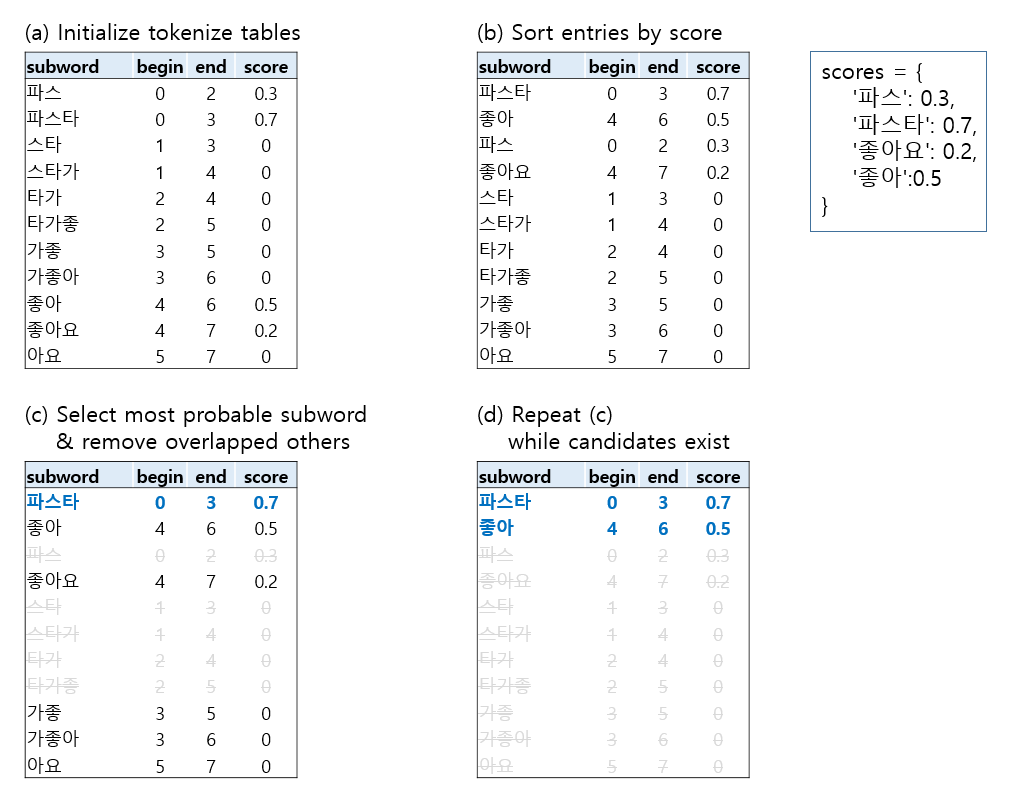
\includegraphics[keepaspectratio=true, width=0.7\linewidth]{figures/maxscoretokenizer.png}
\label{fig:maxscoretokenizer}    
\end{figure}

이처럼 데이터의 띄어쓰기 오류 수준에 따라 서로 다른 전략의 토크나이저를 선택할 수 있다.
L-Tokenizer 는 어절이 L + [R] 로 이분된다는 사실을 사전 지식으로 이용하는 것과 같다.
또한 두 토크나이저 모두 문장에서 부분단어를 잘라내고 단어 점수를 확인하는 작업으로만 이뤄져 있기 때문에 확률 모델을 이용하는 토크나이저들과 비교하여 계산량이 매우 작다.


%%%%%%%%%%%%%%%%%%%%%%%%%%%%%%%%%%%%%%%%%%%%%%%%%
\subsection{성능 평가}
한국국립국어원에서 배포하는 세종 말뭉치에는 문장 원문과 이를 구성하는 형태소가 태깅되어 있으며 \citep{kim200121st}, 다양한 한국어 형태소 분석기들은 세종 말뭉치의 품사 구조를 변형하거나 각자의 단어 사전을 추가하여 배포되고 있다.
형태소 분석기들의 성능을 향상하기 위한 연구에서도 세종 말뭉치는 평가 데이터로 자주 이용된다.
하지만 제안하는 방법은 미등록단어가 자주 발생하는 환경에서 사용하기 위한 방법이기 때문에 세종 말뭉치를 이용한 실험에서는 이러한 환경을 재현하기가 어렵다.
또한 WPM 을 비롯한 비지도학습 기반 단어 추출 방법은 특정 주제의 문서 집합이나 특정 날짜의 뉴스와 같이 텍스트 데이터의 주제가 한정적일 때 잘 작동한다.
하지만 세종 말뭉치는 다양한 종류의 문서로부터 다양한 단어와 패턴을 학습하기 위한 데이터로, 단어 추출기가 잘 작동하는 데이터가 아니다 \citep{kim2014kr}.
또한 띄어쓰기도 잘 지켜지고 있는 데이터이기 때문에 토크나이저가 이용되는 환경과 차이가 있다.
그렇기 때문에 미등록단어 문제와 띄어쓰기 오류가 빈번한 온라인 공간에서 수집한 영화평 데이터를 이용하여 제안하는 모델의 성능을 평가하였다.
네이버 영화로부터 각 영화의 영화평이 5000 개 이상 기록된 152 개의 영화로부터 약 320 만개의 영화평을 수집하였다.
영화평에는 다양한 슬랭 표현 및 배우, 영화 속 캐릭터, 영화 제목과 같은 다양한 고유 명사가 포함되어 있으며, 이들을 제대로 인식하는 것은 영화평 분석의 품질에 큰 영향을 준다.

토크나이저의 성능 평가의 접근법은 정답 단어를 이용하여 결과의 품질을 직접 평가하는 방법과 토크나이저 결과를 이용하는 다른 자연어처리 과업의 성능을 통하여 간접적으로 평가하는 두 가지로 나뉘어진다.
특히 토크나이저는 그 자체가 자연어처리의 최종 과업이 아닌 경우가 많기 때문에 후자의 접근법이 자주 이용된다 \citep{chung2009unsupervised}.
온라인 공간에서 수집한 영화평 데이터를 이용하여 세 종류의 자연어처리 과업을 수행하였다.
첫째는 영화평과 평점을 이용한 감성 분석으로, 이를 통하여 각 토크나이저의 문장에 대한 벡터 표현 능력을 평가한다.
둘째는 고유 명사의 재현율 측정으로, 각 영화에 등장한 배우나 캐릭터명과 같은 정보는 메타데이터로부터 충분히 수집할 수 있다.
또한 이들은 기학습된 형태소 분석기에 등록되지 않은 고유명사일 가능성이 높다.
이들의 재현율을 측정함으로써 미등록단어의 인식 능력을 평가한다.
셋째는 단어 임베딩을 통한 유사 단어 검색 과업이다.
토크나이징의 결과가 문맥을 보존하는 단어열이라면 단어 임베딩 벡터 역시 잘 학습되어 영화 배우의 유사어는 영화 배우로 검색이 되어야 한다.
영화 배우의 이름에 대해서는 메타 데이터로부터 정확한 사전을 구할 수 있기 때문에 영화 배우 이름의 유사어가 실제로 영화 배우의 이름인지 확인하였다.

KoNLPy 는 파이썬 환경에서 다양한 한국어 형태소 분석기를 이용할 수 있도록 도와주는 라이브러리이다 \citep{konlpy}.
그 중 트위터 한국어 분석기는 세종 말뭉치 뿐 아니라 한국어로 작성된 트윗을 분석할 수 있는 단어 사전을 포함하고 있다.
또한 문장 분석 속도도 매우 빠르기 때문에 \citep{konlpy}, 지도학습 기반 형태소 분석기로 이를 비교 실험에 이용하였다.

WPM 은 토크나이저가 이용하는 유닛의 개수를 사용자가 직접 정해야 한다 \citep{wu2016google}.
유닛의 개수에 따른 성능의 차이를 확인하기 위하여 3,000 개부터 50,000 개로 유닛의 개수를 다르게 설정하며 실험을 진행하였다.
이후 WPM3000 은 3,000 개의 유닛을 이용하는 WPM 모델을 의미한다.
제안하는 방법은 Cohesion 점수만 이용하는 경우와 Branching Entropy 를 함께 이용하는 두 경우를 모두 비교하였다.
각각의 모델을 'Cohesion' 과 'CSBE' 로 표기한다.
또한 띄어쓰기만을 이용하는 토크나이저도 비교 실험에 이용하였다.

\subsubsection{영화평을 이용한 긍부정 분류 성능 평가}
영화평에는 1 부터 10 점까지 평점이 함께 부여되어 있다.
평점은 개인마다 기준이 다를 수 있기 때문에 점수를 그대로 이용하기 보다는 긍정과 부정으로 범주화 하여 이용하는 것이 좋다 \citep{pang2008opinion, pang2002thumbs}.
1 \~ 3 점을 부정으로, 8 \~ 10 점을 긍정으로, 그 외의 점수는 개인의 편차가 클 수 있기 때문에 이용하지 않았다.
\citep{wang2012baselines, joulin2016bag} 는 Bigram 과 로지스틱 리그레션 모델 혹은 나이브 베이지안 모델을 이용하는 모델을 문서 분류의 기본 모델로 이용할 것을 제안하였다.
이에 따라 L2 정규화를 이용하는 로지스틱 리그레션 모델에 Unigram 만 이용하는 경우와 Uni, Bigram 을 함께 이용하는 두 경우의 모델을 이용하였으며, 교차 검증 (cross validation) 을 통하여 일반화 성능을 측정하였다.

\begin{table}[ht]
\centering
\caption{Unigram 과 Uni + Bigram 을 이용한 영화평의 긍부정 분류 과업 성능}
\label{tab:sentiment_performance}
%\resizebox{\textwidth}{!}{%
\begin{tabular}{|
>{\columncolor[HTML]{EFEFEF}}c |c|c|c|c|}
\hline
\cellcolor[HTML]{EFEFEF} & \multicolumn{2}{c|}{\cellcolor[HTML]{EFEFEF}\textbf{unigram}} & \multicolumn{2}{c|}{\cellcolor[HTML]{EFEFEF}\textbf{uni + bigram}} \\ \cline{2-5} 
\multirow{-2}{*}{\cellcolor[HTML]{EFEFEF}\textbf{model}} & \cellcolor[HTML]{EFEFEF}\textbf{accuracy} & \cellcolor[HTML]{EFEFEF}\textbf{rank} & \cellcolor[HTML]{EFEFEF}\textbf{accuracy} & \cellcolor[HTML]{EFEFEF}\textbf{rank} \\ \hline
\textbf{WPM3000} & 89.12\% & 10 & 92.67\% & 9 \\ \hline
\textbf{WPM5000} & 89.56\% & 9 & 92.95\% & 8 \\ \hline
\textbf{WPM10000} & 91.69\% & 8 & {\color[HTML]{9A0000} \textbf{93.47\%}} & {\color[HTML]{9A0000} \textbf{3}} \\ \hline
\textbf{WPM20000} & 92.23\% & 4 & 93.41\% & 4 \\ \hline
\textbf{WPM30000} & {\color[HTML]{3166FF} \textbf{92.43\%}} & {\color[HTML]{3166FF} \textbf{2}} & 93.35\% & 6 \\ \hline
\textbf{WPM50000} & {\color[HTML]{3166FF} \textbf{92.65\%}} & {\color[HTML]{3166FF} \textbf{1}} & 93.32\% & 7 \\ \hline
\textbf{Cohesion} & {\color[HTML]{3166FF} \textbf{92.27\%}} & {\color[HTML]{3166FF} \textbf{3}} & {\color[HTML]{9A0000} \textbf{93.48\%}} & {\color[HTML]{9A0000} \textbf{2}} \\ \hline
\textbf{CSBE} & 92.05\% & 5 & {\color[HTML]{9A0000} \textbf{93.63\%}} & {\color[HTML]{9A0000} \textbf{1}} \\ \hline
\textbf{띄어쓰기} & 92.04\% & 6 & 92.13\% & 10 \\ \hline
\textbf{트위터 한국어 분석기} & 91.91\% & 7 & 93.39\% & 5 \\ \hline
\end{tabular}%
%}
\end{table}

표 \ref{tab:sentiment_performance}은 토크나이저 별 영화평의 긍부정 분류 성능이다.
긍부정 분류에서는 Bigram 이 중요한 정보를 표현한다.
단어 '재미'는 긍부정을 명확히 표현하지 못하지만 '재미 + 없다'는 이를 표현할 수 있다.
하지만 토크나이저들은 '재미없다'를 '재미 + 없다'로 구분하기 때문에 Bigram 을 함께 이용하는 경우 Unigram 만 이용하는 경우보다 성능이 증가함을 확인할 수 있다.

제안된 방법은 트위터 한국어 분석기보다 높은 성능을, 많은 수의 유닛을 이용하는 WPM 과도 비슷한 성능을 보인다.
특히 제안하는 모델이 Bigram 을 이요하는 경우에 가장 높은 성능을 보이는데, 이는 영화평 도메인에서 사용되는 표현들을 잘 인식함을 의미한다.

띄어쓰기를 토크나이저로 이용하는 경우에는 Unigram 을 이용하는 경우와 Bigram 을 함께 이용하는 경우의 성능 차이가 거의 없는데, 이는 Unigram 안에 이미 '재미없다'와 같은 어절이 포함되어 있기 때문이다.
그리고 이 성능은 트위터 한국어 분석기의 Unigram 을 이용하는 경우보다도 높게 나타났다.

유닛의 개수가 작은 WPM 은 Bigram 을 함께 이용할 때 성능이 향상되지만, 유닛의 개수가 많은 WPM 은 Bigram 을 함께 이용하여도 성능 향상이 잘 이뤄지지 않는다.
이는 적은 유닛의 WPM 을 이용하여 생성된 Bigram 이 많은 유닛을 이용하는 WPM 의 유닛인 경우가 많기 때문이다.
실제로 WPM3000 에서 Bigram 을 함께 이용한 경우, 단어 문서 행렬의 차원이 약 54k 이었다.

그 외 다른 판별 모델을 이용하여도 영화평의 긍부정 판별의 성능은 93 \% 후반을 넘기기 어려웠는데, 이는 영화평 데이터에는 '드디어 개봉했네'처럼 긍부정을 판단하기 어려운 짧은 문장들이 포함되어 있기 때문이다.


\subsubsection{메타 데이터를 이용한 고유 명사 재현 능력 평가}
영화평 데이터에 등장하는 다양한 단어들을 정확히 알 수는 없지만, 메타데이터로부터 영화 배우의 이름, 극 중 캐릭트 명, 영화 제목과 같은 일부 고유 명사에 대한 리스트를 만들 수 있다.
각 토크나이저들이 이들을 제대로 인식할 수 있는지 평가하였다.
'한효주'는 리뷰와 메타 데이터에 자주 등장하는 배우 이름이며, 이는 '한효주 + 가', '한효주 + 의' 처럼 조사와 결합되어 이용된다.
그러나 '한효주'가 기학습된 형태소 분석기의 사전이나 WPM 의 유닛으로 등록되어 있지 않다면 '한효 + 주가'나 '한효 + 주의' 처럼 잘못된 단어열로 분해될 수 있다.

표 \ref{tab:metamatching} 는 영화평 데이터에 각각의 토크나이저를 적용한 뒤, 메타 데이터에 등록된 고유 명사가 단어로 존재하는지 확인한 결과이다.
트위터 한국어 분석기에는 유명한 영화 배우의 이름들이 등록되어 있기 때문에 배우 이름에서 높은 인식능력을 보이지만, 극중 캐릭터 명이나 영화 제목은 미등록 단어일 가능성이 높다.
제안하는 방법은 데이터에 자주 등장하는 단어들을 추출하기 때문에 배우 이름 뿐 아니라 캐릭터 명이나 영화 제목을 제대로 인식할 수 있다.
제안하는 방법은 모든 종류의 단어에서 사전을 이용하는 트위터 한국어 분석기와 비슷한 단어 인식 능력을 보임을 확인할 수 있다.
그러나 WPM 의 경우 유닛의 개수를 증가하여도 인식되는 고유 명사의 개수가 적었다.
이는 WPM 의 문장의 분해 단위가 단어가 아닌, 자주 등장하는 부분단어이기 때문이다.
WPM 은 유닛의 개수를 증가하면 새로운 단어를 유닛으로 추가하는 것이 아니라, 자주 등장하는 어절을 유닛으로 추가한다.

\begin{table}[ht]
\centering
\caption{토크나이저 별 고유 명사 재현율 (배우 이름, 영화 제목, 극 중 캐릭터 이름)}
\label{tab:metamatching}
%\resizebox{\textwidth}{!}{%
\begin{tabular}{|
>{\columncolor[HTML]{EFEFEF}}c |c|c|c|}
\hline
\textbf{model} & \cellcolor[HTML]{EFEFEF}\textbf{배우 이름} & \cellcolor[HTML]{EFEFEF}\textbf{영화 제목, 극 중 캐릭터 이름} & \cellcolor[HTML]{EFEFEF}\textbf{전체} \\ \hline
\textbf{WPM3000} & 0 & 0.13 & 0.05 \\ \hline
\textbf{WPM5000} & 0 & 0.13 & 0.05 \\ \hline
\textbf{WPM10000} & 52.05 & 27.21 & 43.3 \\ \hline
\textbf{WPM20000} & 63.93 & 50.42 & 59.17 \\ \hline
\textbf{WPM30000} & 65.99 & 54.49 & 61.94 \\ \hline
\textbf{WPM50000} & 63.21 & 56.62 & 60.89 \\ \hline
\textbf{Cohesion} & {\color[HTML]{00009B} \textbf{82.23}} & {\color[HTML]{00009B} \textbf{71.29}} & {\color[HTML]{00009B} \textbf{78.38}} \\ \hline
\textbf{CSBE} & {\color[HTML]{00009B} \textbf{88.4}} & {\color[HTML]{00009B} \textbf{82.08}} & {\color[HTML]{00009B} \textbf{86.17}} \\ \hline
\textbf{띄어쓰기} & 36.09 & 31.09 & 34.33 \\ \hline
\textbf{트위터 한국어 분석기} & {\color[HTML]{00009B} \textbf{92.95}} & {\color[HTML]{00009B} \textbf{77.14}} & {\color[HTML]{00009B} \textbf{87.38}} \\ \hline
\end{tabular}%
%}
\end{table}

\subsubsection{단어 임베딩을 이용한 유사 단어 검색 성능 평가}
토크나이징의 결과가 문맥을 보존하는 단어열이라면 단어 임베딩 벡터 역시 잘 학습되어 영화 배우의 유사어는 영화 배우로 검색이 되어야 한다.
영화평에 각 토크나이저를 적용한 뒤, Word2Vec \citep{mikolov2013efficient} 을 이용하여 단어 임베딩 벡터를 학습하였다.
단어 임베딩 모델은 단어의 빈도수가 작으면 학습이 잘 이뤄지지 않기 때문에 최소빈도수 10 을 넘는 단어만을 학습에 이용하였다.
메타 데이터에 등록된 영화 배우의 이름을 입력하여 상위 10 개의 유사어를 검색한 뒤, 이들이 배우 이름인지 확인하였다.

표 \ref{tab:word2vec_actor} 의 첫번째 열은 토크나이저에 의하여 재현된, 빈도수 10 이상의 배우 이름의 개수이다.
사전을 이용하는 트위터 한국어 분석기와 Cohesion 을 이용하는 모델은 800 명이 넘는 이름을 제대로 인식하였음을 확인할 수 있다.
두번째 열은 유사어가 실제로 배우 이름인 비율이며, 세번째 열은 검색된 유사어의 빈도수를 고려한 가중 평균이다.
트위터 한국어 분석기를 이용한 경우 가장 좋은 성능을 보이는데, 이는 트위터 한국어 분석기를 이용하는 경우 문맥이 잘 보존된다고 해석할 수 있다.

\begin{table}[ht]
\centering
\caption{단어 임베딩 벡터를 이용하여 검색된 배우 이름의 유사어 중 배우 이름인 비율}
\label{tab:word2vec_actor}
%   \resizebox{\textwidth}{!}{%
\begin{tabular}{|
>{\columncolor[HTML]{EFEFEF}}c |c|c|c|}
\hline
\textbf{model} & \cellcolor[HTML]{EFEFEF}\textbf{재현된 단어 개수} & \cellcolor[HTML]{EFEFEF}\textbf{\begin{tabular}[c]{@{}l@{}}유사어 중\\배우 이름 비율\end{tabular}율} & \cellcolor[HTML]{EFEFEF}\textbf{\begin{tabular}[c]{@{}l@{}}단어 빈도수를 고려한\\유사어 중 배우 이름 비율\end{tabular}} \\ \hline
\textbf{WPM3000} & 0 & 0 & 0 \\ \hline
\textbf{WPM5000} & 0 & 0 & 0 \\ \hline
\textbf{WPM10000} & 64 & 59.06 & 75.67 \\ \hline
\textbf{WPM20000} & 159 & 66.54 & 77.71 \\ \hline
\textbf{WPM30000} & 220 & 67.27 & 76.2 \\ \hline
\textbf{WPM50000} & 309 & 63.66 & 73.97 \\ \hline
\textbf{Cohesion} & 847 & 54.91 & 73.64 \\ \hline
\textbf{CSBE} & 649 & 58.72 & 71.21 \\ \hline
\textbf{띄어쓰기} & 696 & 45.22 & 68.93 \\ \hline
\textbf{트위터 한국어 분석기} & 822 & 64.77 & 80.87 \\ \hline
\end{tabular}%
%   }
\end{table}

또한 제안하는 방법들을 포함한 WPM 도 트위터 한국어 분석기와 비슷하거나 조금 낮은 문맥 보존 능력을 보인다.
하지만 WPM 은 단어 임베딩에 이용된 배우의 이름 개수 자체가 상대적으로 매우 적다.
이는 일부의 단어에 대해서만 제대로 인식되고, 많은 단어들이 문맥 정보를 잘 반영하지 못하는 단위로 나뉘어졌음을 의미한다.


%%%%%%%%%%%%%%%%%%%%%%%%%%%%%%%%%%%%%%%%%%%%%%%%%
\subsection{결론}
이 논문은 한국어의 어절 구조를 L + [R] 로 가정한 뒤, 미등록단어가 발생하는 L 부분의 단어를 통계 기반으로 추출하는 방법과 이를 이용하는 비지도학습 기반 토크나이저를 제안하였다.
제안하는 방법은 데이터의 띄어쓰기 오류 수준에 따라서 L-Tokenizer 와 Max Score Tokenizer 를 선택할 수 있다.
제안하는 방법은 온라인 공간에서 수집된 영화평 데이터를 이용하여 성능을 평가하였다.
문장의 긍부정 판별, 고유 명사의 인식, 단어 임베딩을 이용한 유사어 검색 과업을 통하여 제안하는 방법은 WPM 보다도 좋은 단어 인식 능력 및 문서의 벡터 표현 능력이 있으며, 사전을 이용하는 트위터 한국어 분석기와도 비슷한 토크나이징 능력이 있음이 확인되었다.

그러나 음절 단위의 언어모델은 데이터의 부분단어가 모호성이 없을 때 잘 작동한다.
뉴스 데이터에서는 '카메라'라는 단어가 자주 등장하며 나라 이름 '카메룬'은 상대적으로 적게 등장하는데, 이 경우에는 $P$(카메룬 $\vert$ 카메) 의 값이 매우 작기 때문에 오히려 cohesion('카메') $\le$ cohesion('카메룬')이 되며, '카메룬'의 Branching Entropy 가 이를 상쇄할만큼 크지 않다면, '카메룬의 = 카메 + 룬의'로 잘못 분리된다.
이를 해결하기 위해서는 R 의 정보를 함께 이용하여 '카메룬 + 의'의 토크나이징 점수가 '카메 + 룬의'의 토크나이징 점수보다 크도록 정의할 수 있어야 한다.

혹은 가능하다면 주제가 동일한 문서만을 나눠서 Cohesion 점수를 학습하는 것이 좋다.
아프리카와 관련된 뉴스들에 대해서만 Cohesion 을 학습하였다면 '카메룬'의 빈도수가 충분하여 높은 점수를 얻을 수 있다.
영화 리뷰에서는 영화 별로 리뷰를 나눠서 Cohesion 과 Branching Entropy 를 학습할 수도 있다.

제안된 방법은 단어 사전의 구축을 위하여 전문가의 수작업을 요구하지 않기 때문에, 한국어의 어절 구조가 유지되는 임의의 도메인에 적용할 수 있으며, 간단한 계산 과정만으로 토크나이징이 가능하기 때문에 대량의 문서 집합에 적용하기에 용이하다.
또한 기존의 \citep{zhao2007incorporating, zhao2011integrating, zheng2013deep} 연구들처럼 기학습된 모델의 미등록단어 인식 성능을 보완하는데 이용될 수도 있다.
그러나 앞서 언급한 것처럼 음절 단위의 언어모델은 빈도수가 작은 일부 단어들에 대해서 단어 점수가 제대로 학습되지 않는 단점이 있다.
이러한 점을 보완한다면 미등록단어 문제를 해결하는 더 좋은 토크나이저로 발전할 것으로 기대한다.



%%%%%%%%%%%%%%%%%%%%%%%%%%%%%%%%%%%%%%%%%%%%%%%%%%%%%%%%%%%%%%%%%%%%%%%%%%%%%%%
\newpage
\section{어절 구조를 이용한 통계 기반 명사 추출} \label{noun_extraction}

\subsection{개요}

단어는 의미를 표현하며 새로운 단어가 만들어지는 열린 집합과 문법 기능을 수행하는 닫힌 집합으로 분류할 수 있다.\citep{jurafsky2000speech}.
열린 집합의 단어는 새로운 단어가 만들어지기 때문에 미등록단어 문제가 발생한다.
한국어에서 명사는 가장 많이 이용되는 단어로, 세종 말뭉치의 29.12 \% 에 해당하며, 형태소 어미, 조사, 동사와 형용사의 어간이 각각 19.17 \%, 17.11 \%, 13.53 \% 씩 등장한다 (표 \ref{tab:pos_statistics}).
또한 명사는 가장 많은 종류의 단어로 구성된 집합이다.
세종 말뭉치의 통계에서 약 14만여종의 명사가 각각 평균적으로 49 번 정도 등장함에 비하여 289 종의 조사는 약 1만 4천번 정도 등장함을 확인할 수 있다.
이는 명사의 다양성이 매우 큼을 의미한다.

\begin{table}[ht]
  \centering
  \caption{세종 말뭉치의 형태소 품사 별 통계}
  \label{tab:pos_statistics}
%\resizebox{\textwidth}{!}{
\begin{tabular}{|>{\columncolor[HTML]{EFEFEF}}c |c|c|c|}
\hline
\textbf{형태소 품사}  & \cellcolor[HTML]{EFEFEF}\textbf{출현 빈도수 (비율)} & \cellcolor[HTML]{EFEFEF}\textbf{고유 개수} & \cellcolor[HTML]{EFEFEF}\textbf{평균 출현 빈도수} \\ \hline
\textbf{명사} & 7,124,644 (29.128\%) & 144,294 & 49.38 \\ \hline
\textbf{용언의 어미} & 4,688,406 (19.168\%) & 3,142 & 1,492.17  \\ \hline
\textbf{조사} & 4,184,235 (17.107\%) & 289  & 14,478.32 \\ \hline
\textbf{용언의 어간} & 3,308,743 (13.527\%) & 7,989 & 414.16  \\ \hline
\end{tabular}
%}
\end{table}

유의미한 텍스트 분석을 위해서 명사는 다른 품사들보다도 우선적으로 정확히 인식되어야 한다.
키워드를 이용한 문서 요약이나 토픽 모델링은 단어 분포를 이용하여 그 결과를 해석한다.
명사가 제대로 인식되지 않으면 주요한 단어들이 생략되어 분석 결과의 품질이 떨어진다.

문장을 단어로 인식하는 과정에서 품사 판별기나 형태소 분석기가 이용된다.
특히 형태소 분석기는 "학습데이터에 등장하지 않은 단어는 알려진 형태소의 조합으로 구성"된다고 가정한다.
하지만 한국어는 한자를 이용하는 언어이기 때문에 각 음절이 단어인 경우가 많으며, 이는 미등록단어를 여러개의 짧은 형태소로 분해하는 결과를 야기한다.
또한 한국어에서 이용되는 음절의 수가 작기 때문에 음절 간의 모호성이 발생한다.
세종 말뭉치에서는 300 글자가 말뭉치 전체의 89.48 \% 를, 1,000 글자가 말뭉치 전체의 96.08 \% 를 차지하며, 이들로부터 수백만개의 단어가 형성된다.
표 \ref{tab:ioisentence_postagging_example} 는 기학습된 형태소 분석기인 꼬꼬마와 트위터 한국어 처리기를 이용하여 예문 '아이오아이는 걸그룹 이름이다'의 형태소 분석을 한 결과이다.
두 모델에는 '아이오아이'가 학습데이터에 등장하지 않았기 때문에 '아이오'와 '아이'라는 두 명사로 분해하였다.

\begin{table}[ht]
\centering
\caption{기학습된 한국어 형태소 분석기를 이용한 문장 분석 예시. (N: 명사, J: 조사, V: 동사, E: 어미, VCP: 동사형 전성어미)}
\label{tab:ioisentence_postagging_example}
\resizebox{\textwidth}{!}{%
\begin{tabular}{|l|l|} \hline
\textbf{정답 단어열} & 아이오아이/N + 는/J + 걸그룹/N + 이름/N + 이다/V \\ \hline
\textbf{꼬꼬마 형태소 분석기} & 아이오/N + 아이/N + 는/J 걸/N + 그룹/N + 이름/N + 이/VCP + 다/E \\ \hline
\textbf{트위터 한국어 처리기} & 아이오/N + 아이/N + 는/J + 걸그룹/N + 이름/N + 이다/J \\ \hline
\end{tabular}
}
\end{table}

조건부 임의 필드 (Conditional Random Field) 나 히든 마르코프 모델 (Hidden Markov Model) 과 같은 순차적 레이블링 알고리즘을 이용하는 모델들은 앞 뒤에 등장하는 단어를 이용하여 미등록단어의 품사를 추정할 수 있는 능력이 있다 \citep{shim2004high, shim2007made, na2012crfs, lee2013joint}.
그러나 모든 단어 후보에 대해 품사를 추정하는 것은 계산량이 많고 부정확한 추정을 할 수 있기 때문에 품사 판별기와 형태소 분석기는 단어 사전을 이용한다.

이러한 문제를 해결하기 위해서는 사용자에 의한 사전 추가가 필요하다.
하지만 새로운 도메인의 문서를 분석하기 전에는 어떠한 단어가 이용되는지 예상하기 어렵기 때문에, 현실적으로는 문서 분석 후 잘못 분해된 단어를 후처리 작업을 수행한다.

그러나 명사의 오른쪽에 등장하는 단어들의 분포를 이용하면 명사 추출도 가능하다 \citep{Lee2016functional}.
그림 \ref{fig:fig1_aexample} 의 예문에서 단어 'A'의 오른쪽에는 '-는', '-에서', '-로' 와 같이 자주 이용되는 조사들이 등장한다.
이러한 정보를 바탕으로 단어 'A'가 명사라고 추정할 수 있다.

\begin{figure}[ht]
\centering
\caption{A가 포함된 문장 예시}
\label{fig:fig1_aexample}
\begin{tabular}{|l|}
\hline
\begin{tabular}[c]{@{}l@{}}문장 1: "A는 좋아"\\ 문장 2: "A에서 만나"\\ 문장 3: "A로 가자"\end{tabular} \\ \hline
\end{tabular}
\end{figure}

이 장에서는 어절의 오른쪽에 등장하는 부분어절의 분포를 이용하여 데이터 기반으로 명사를 추출하는 방법을 제안한다.
한 어절에서 명사 오른쪽에는 빈칸, 조사들이 자주 등장하며, 표 \ref{tab:pos_statistics} 에서 살펴볼 수 있듯이 조사의 종류는 제한적이기 때문에 이를 명사 추출의 변수로 이용할 수 있다.
또한 조사는 닫힌 집합에 속하는 단어이기 때문에 도메인에 상관없이 명사를 추출하는 정보로 이용할 수 있다.


%%%%%%%%%%%%%%%%%%%%%%%%%%%%%%%%%%%%%%%%%%%%
\subsection{관련 연구}

조건부 임의 필드나 구조적 지지 벡터 머신같은 순차적 레이블링 알고리즘은 새로운 단어의 품사를 추정할 수 있다. \citep{shim2004high, shim2007made, na2012crfs, lee2013joint}.
순차적 레이블링의 식 \ref{eq:transition_based_tagger_i} 에서 단어 후보 $x_i$ 의 품사를 추정하는 정보로 앞 뒤에 등장하는 단어인 $(x_{i-1}, t_{i-1}, x_{i+1}, t_{i+1})$ 를 이용하여 $x_i$ 의 품사를 한다 \citep{shim2004high, shim2007made, na2012crfs, lee2013joint}.
순차적 레이블링 알고리즘은 $x_i$ 가 여러 개의 품사를 지닐 때 뿐 아니라 $x_i$ 가 사전에 등록된 단어가 아닐 때에도 문맥을 고려하여 적합한 품사 $t_i$ 를 추정한다.
하지만 형태소 분석이나 품사 추정 과정에서 가능한 모든 단어 후보 $x_i$ 에 대하여 품사를 추정하는 것은 지나치게 큰 계산 비용이 든다.
그렇기 때문에 현실적으로는 문맥 정보는 사전에 등장한 단어 후보 $x_i$ 가 여러 개의 품사를 지니는 모호성을 해결하는데에만 이용된다.
또한 학습데이터에 존재하는 단어만 문맥정보 $x_{i-1}, x_{i+1}$ 로 이용할 수 있다.

규칙 기반으로 한국어의 미등록단어 문제를 해결하려는 연구도 제안되었다.
단어의 앞음절 (prefix) 이나 뒷음절 (suffix) 을 기반으로 품사를 추정하는 방법 \citep{Lee2016functional} 과 음절 단위의 템플릿 기반으로 새로운 단어를 인식하는 방법 \citep{hong2008new} 이 제안되었다.
하지만 템플릿 기반 방법은 새로운 단어에 템플릿의 음절이 포함되어 있을 경우 실패하는 경우가 많다.
예를 들어 “$\sim$/명사 + 은/조사' 템플릿은 '은'으로 끝나는 명사를 잘못 인식하게 되는데, 명사는 그 자체로 어절을 이루는 경우가 존재하기 때문에 '손나은'이라는 고유 명사가 '손나'처럼 잘못 인식되는 경우가 발생한다.
이를 해결하기 위하여 예외 규칙과 오토마타를 이용한 명사 추출 방법도 제안되었지만 \citep{lee2003efficient}, 이는 오토마타에 포함된 규칙에 해당하는 명사만 추출할 수 있다는 단점이 있다.
예를 들어 'ㅆ' 이나 'ㄺ' 은 명사에 자주 등장하지 않는 자음이기 때문에 이러한 자음이 포함된 신조어들은 규칙 기반으로 추출될 수 없다.

단어 임베딩은 같은 품사의 단어를 탐색하는데 이용될 수 있다.
단어 임베딩 벡터는 의미가 비슷한 단어를 비슷한 벡터로 표현할 뿐 아니라, 같은 품사의 단어들 역시 비슷한 벡터로 표현한다 \citep{bengio2003neural}.
그렇기 때문에 Word2Vec 과 같은 모델을 이용하여 단어 임베딩 벡터를 학습한 뒤, 알려진 명사를 이용하여 명사를 확장할 수 있다 \citep{mikolov2013distributed} .
하지만 Word2Vec 은 문장이 단어열로 정확히 나뉘어져 있다고 가정하는데, 한국어는 교착어이며 띄어쓰기 오류가 포함된 경우가 많기 때문에 토크나이징이 이뤄지지 않으면 단어 임베딩 벡터를 학습할 수 없다.
FastText \citep{bojanowski2017enriching} 는 토크나이저를 이용하지 않는 단어 임베딩 방법이지만, 이 방법은 단어의 형태적 유사성과 문맥을 함께 보존하는 단어 임베딩 방법이기 때문에 명사의 유사어로 어절이 등장하는 경우가 많다.

그러나 그림 \ref{fig:fig1_aexample} 에서 볼 수 있듯이 어절 내의 단어 분포 정보를 이용하면 명사를 쉽게 추정할 수 있다.
\citep{shim2016cloning} 학습된 형태소 분석기의 복제 실험을 수행하였는데, 앞 뒤 문맥을 모두 이용하는 형태소 분석기를 이용하여 어절들을 분석한 뒤 어절을 형태소열로 변환하는 함수를 학습하였다.
이는 앞 뒤에 등장하는 단어들을 변수로 이용하지 않음을 의미하는데, 그럼에도 불구하고 98.31 % 의 재현율을 보였다.
즉 다수의 어절의 형태소 분석은 그림 \ref{fig:fig1_aexample} 처럼 한 어절 내에서 가능함을 의미하며, 이러한 관점은 명사 추출에도 이용될 수 있다.




%%%%%%%%%%%%%%%%%%%%%%%%%%%%%%%%%%%%%%%%%%%%
\subsection{제안하는 방법}

주어진 문서 집합에서 어절의 구조적 특징과 통계를 이용하여 명사를 추출하는 알고리즘을 제안한다.
이는 수작업으로 명사 사전을 구축하는 비용을 줄여줄 뿐 아니라, 수작업에 의하여 놓치기 쉬운 단어들도 사전에 포함할 수 있다는 장점이 있다.
한국어의 어절은 그림 \ref{fig:korean_structure} 처럼 여러 개의 복합 형태소로 구성되어 있다.
하지만 단어 추출을 위해서는 어절 구조를 단순한 구조로 정의해야 한다.
이를 위하여 단어 추출을 위한 단순화된 한국어 어절 구조를 제안하고, 이 구조를 이용한 명사 추출 방법을 설명한다.

\subsubsection{L-R 그래프를 이용한 명사 추출기}

제안하는 명사 추출 방법은 한국어 어절의 L + [R] 구조를 이용한다.
명사는 의미를 지니기 때문에 L 에 해당하며, R 로는 조사와 그 외의 복합 형태소가 등장한다.
명사는 전성어미와 결합되어 동사나 형용사로 이용될 수 있는데, 이 때 사용되는 전성어미는 '-하, -되, -이, -있' 처럼 제한적이며 동사나 형용사의 어간과 같은 형태이다.
즉 형태적으로는 명사의 오른쪽에 조사와 용언의 표현형이 등장할 수 있으며, 이들의 종류는 제한적이다.
용언은 어간이 포함된 음절이 L 에 해당하며 R 로는 어미 혹은 어미가 포함된 복합형태소가 등장한다.
그 외의 품사는 한 형태소가 하나의 어절을 이룬다.
그렇기 때문에 한 어절을 (L, R) 로 분해한 뒤, R 을 이용하여 L 이 명사인지 판별할 수 있다.

각 어절마다 독립적으로 L 이 명사인지 판단하는 것은 템플릿을 이용하는 것과 같다.
그림 \ref{fig:fig1_aexample} 에서 'A' 를 명사로 추정할 수 있는 근거는 모든 문장에서의 'A' 에 대한 R 분포다.
한 단어 L 이 명사라면 R 에 다양한 조사와 용언이 분포하며, L 이 용언이라면 R 에 다양한 어미들이 분포할 것이다.
이처럼 데이터의 모든 어절의 전역적인 정보를 이용하면 정확한 단어의 추정이 가능하다 \citep{zhao2007incorporating}.

그러나 어절이 주어졌을 때 L 과 R 의 경계를 알지 못한다.
제안하는 모델은 이러한 문제를 해결하기 위하여 그림 \ref{fig:noun_diagram} 같이 세 단계로 구성되어 있다.

\begin{figure}[ht]
\centering
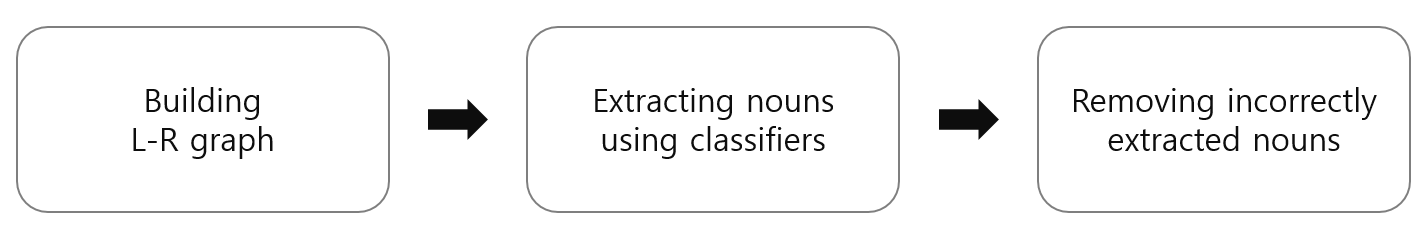
\includegraphics[keepaspectratio=true, width=0.5\linewidth]{figures/noun_diagram.png}
\label{fig:noun_diagram}
\caption{제안하는 명사 추출기의 프레임워크}
\end{figure}

첫 단계에서는 주어진 모든 어절을 가능한 조합으로 이분하여 L-R 그래프를 만든다.
어절 내에 R 이 없을 수도 있기 때문에 그림 \ref{fig:four_lrcandidates} 처럼 한 어절이 L 이 될 수도 있다.
어절 '드라마를'은 네 종류의 (L, R) 쌍으로 분해되며, 데이터의 모든 (L, R) 조합의 빈도수를 계산하여 이를 두 마디 L 과 R 사이의 호의 가중치로 정의한다.

\begin{figure}[H]
\small
\centering
\caption{어절 ‘드라마를’로부터 생성할 수 있는 (L, R) 쌍 예시}
\label{fig:four_lrcandidates}
%\resizebox{\textwidth}{!}{%
\begin{tabular}{|c|}
\hline
{[}(드, 라마를), (드라, 마를), (드라마, 를), (드라마를, ''){]} \\ \hline
\end{tabular}%
%}
\end{figure}

'드라마/L'는 명사이기 때문에, 이와 함께 등장한 R 은 조사가 다수이다.
표 \ref{tab:lr_drama_examples} 의 왼쪽 행은 하루의 뉴스 문서 집합에서 학습한 L-R 그래프이다.
'드라마'의 R 에는 '-를' 87 회, '-의' 67 회 처럼 조사들이 다수 등장하며, 용언의 어간인 '시작했/L' 의 R 에는 어미들이 다수 등장함을 확인할 수 있다.

\begin{table}[H]
\small
\centering
\caption{‘드라마/L’ 와 ‘시작했/L’ 를 포함하는 가장 빈번한 (L, R) 쌍 예시}
\label{tab:lr_drama_examples}
%\resizebox{\textwidth}{!}{%
\begin{tabular}{|c|c|}
\hline
\rowcolor[HTML]{EFEFEF} 
\textbf{Ten Most frequent (L, R) structure for ‘드라마’} & \textbf{Ten Most frequent (L, R) structure for '시작했’} \\ \hline
(드라마, ) = 278 & (시작했, 다) = 2900 \\ \hline
(드라마, 를) = 87 & (시작했, 습니다) = 229 \\ \hline
(드라마, 의) = 67 & (시작했, 고) = 170  \\ \hline
(드라마, 가) = 60 & (시작했, 는데) = 75  \\ \hline
(드라마, 는) = 50 & (시작했, 던) = 69   \\ \hline
(드라마, 에) = 47 & (시작했, 다는) = 68  \\ \hline
(드라마, 에서) = 42& (시작했, 을) = 67   \\ \hline
(드라마, 로) = 26 & (시작했, 다고) = 50  \\ \hline
(드라마, 나) = 18 & (시작했, 으며) = 44  \\ \hline
(드라마, 틱한) = 17& (시작했, 어요) = 41  \\ \hline
\end{tabular}%
%}
\end{table}

두번째 단계에서는 학습된 L-R 그래프에서 길이가 2 이상인 L 에 대하여 R 의 빈도수 벡터를 이용한 명사 유무를 판별한다.
한국어는 표의 문자의 성격이 있기 때문에 1음절 단어는 명사인 경우가 많으며, 추출이 되어도 해석이 모호한 경우가 많다.
또한 L 의 빈도수와 R 의 종류가 사용자가 정의한 최소값 이상인 경우에 대해서만 판별 작업을 수행한다.
L 의 단어 후보가 실제로 명사라면 다양한 조사들이 R 에 등장할 것이지만, 한 번 등장한 L 은 R 이 단어의 일부인지 혹은 조사인지를 확인하기 어렵다.
또한 한 종류의 R 과 함께 등장하는 L 은 명사가 아닌 다른 단어의 부분글자일 가능성이 높기 때문이다.
L 의 명사 판별에 이용하는 판별기는 세종 말뭉치를 이용하여 학습한다.
세종 말뭉치를 이용한 판별기 학습에 대한 내용은 다음 장에서 다룬다.

마지막 단계에서는 후처리 과정을 통하여 잘못 추출된 명사를 걸러낸다.
가능한 모든 부분어절 L 에 대하여 명사 유무를 판별했기 때문에 명사 후보에는 단어의 부분글자들이 포함되어 있다.
명사로 잘못 판단된 L 은 세 종류로 분류할 수 있다.
첫번째는 명사의 마지막 어절이 조사와 같은 글자인 경우이며, 이는 “$N_{sub} + J$” 형태이다.
예를 들어 명사 '떢볶이' 는 그 자체로 어절을 이루는 경우가 많으며, '-이'가 포함되어 있기 때문에 “떡볶/명사 + 이/조사” 로 판별될 수 있다.
하지만 '떢볶' 다음에 등장하는 글자는 대부분 '이' 이기 때문에 Branching Entropy 값이 매우 작고, '떢볶이' 다음에는 다양한 조사도 등장하기 때문에 큰 Branching Entropy 값을 지닌다.
이처럼 명사로 추출된 단어의 마지막 음절이 조사에 해당하며 이를 제거한 부분음절 역시 명사로 추출된 경우, Branching Entropy 를 계산하여 그 값이 임계값 (예, 0.5) 보다 작은 부분 어절은 명사가 아닌 것으로 재분류 한다.

두번째 종류는 조사의 일부 글자가 명사에 포함된 경우로, “$N + J_{sub}$” 형태이다.
예를 들어 어절 '대학생과의'는 '대학생/명사 + 과의/조사' 로 구분되어야 한다.
하지만 '-의' 역시 자주 이용되는 조사이기 때문에 '대학생과/명사 + 의/조사' 로 판별되는 경우가 발생한다.
이때는 위의 경우와 반대로 명사 '대학생'은 다른 조사들과 함께 등장한 경우가 많기 때문에 높은 Branching Entropy 를 지니지만 '대학생과' 다음에 등장하는 글자는 대부분 '-의' 이기 때문에 낮은 Branching Entropy 를 지닌다.
그러므로 명사로 추출된 단어의 마지막 음절이 조사의 일부이며 이를 제거한 부분음절 역시 명사로 분류된 경우, 긴 단어의 Branching Entropy 가 임계값 (예, 0.5) 보다 작다면 이를 명사가 아닌 것으로 재분류 한다.

마지막 종류는 복합 명사이다.
어절 '소수집단의' 는 '소수/명사 + 집단/명사 + 의/조사'로 분류되어야 하지만, L-R 그래프에 의하여 '소수집단'이 명사로 추출된다.
만약 '소수'와 '집단'이 자주 이용되는 명사라면 이는 각각 명사로 추출된다.
길이가 긴 명사가 길이가 짧은 다른 명사열로 구성될 경우 이를 분해하여 복합명사를 분리할 수 있다.
하지만 분석 목적에 따라서는 '유엔안전보장이사회'처럼 복합명사를 그대로 이용하기도 한다.
그러므로 마지막 종류의 후처리는 사용자의 선택에 의하여 실행한다.

\subsubsection{세종 말뭉치를 이용한 명사 판별 분류기 학습}

세종 말뭉치는 L-R 그래프에서 L 이 명사인지를 판단하는 판별기를 학습하는데 이용될 수 있다.
세종 말뭉치는 구어체와 문어체의 문서들로 이뤄진 형태소 분석용 말뭉치로, 1,560,437 개의 고유어절이 10,807,777 번 등장하는 1,054,566 문장으로 이뤄진 학습데이터이다.
이 중 명사와 용언이 L 로 위치한 어절을 학습데이터로 이용하였다.

세종 말뭉치는 어절을 형태소 수준으로 분해한 데이터이기 때문에 L + [R] 구조로 변형하였다.
복합 명사는 단일 명사로 변환하며, 전성어미와 명사가 포함된 어절은 전성어미 이후의 복합 형태소를 하나의 단어로 변환하였다.
용언은 어간을 L 로 어미를 R 로 변형하였으며, R 이 복합 형태소일 경우에는 이를 하나의 단어로 변형하였다.
어간이 활용된 경우에는 어간이 포함된 음절을 L 로 정의하였다.

\begin{table}[H]
\centering
\caption{세종 말뭉치의 어절을 L + [R] 구조로 변형한 예시}
\label{tab:lrstructure}
% \resizebox{\textwidth}{!}{%
\begin{tabular}{|c|c|}
\hline
\rowcolor[HTML]{EFEFEF} 
\textbf{형태소 분석 관점} & \textbf{L + [R] 구조 관점} \\ \hline
졸업/N + 논문/N + 의/J & 졸업논문/N + 의/R \\ \hline
시작/N + 하/VCP + 았/E + 다/E & 시작/N + 했다/R \\ \hline
하/V + 았/E + 다/E & 했/V + 다/R \\ \hline
\end{tabular}%
% }
\end{table}

그 결과 197,651 종류의 L 과 22,394 종류의 R 이 생성되었으며, 이들의 최소빈도수가 임계값보다 작은 경우는 데이터에서 제거하였다 (표 \ref{tab:num_of_lr}.
학습데이터의 레이블은 L 이 명사인지의 유무를 이진 벡터로 표현하였다.

\begin{table}[H]
\small
\centering
\caption{L 과 R 의 최소빈도수 이상 조건을 만족하는 단어의 종류}
\label{tab:num_of_lr}
%\resizebox{\textwidth}{!}{%
\begin{tabular}{|c|c|c|}
\hline
\rowcolor[HTML]{EFEFEF} 
\textbf{최소 빈도수} & \textbf{고유 L 개수} & \textbf{고유 R 개수} \\ \hline
\begin{tabular}[c]{@{}c@{}}L \textgreater= 0, R \textgreater= 0 \\ (without filtering)\end{tabular} & 197,651 & 22,394 \\ \hline
L \textgreater= 5, R \textgreater= 5 & 50,233 & 5,361 \\ \hline
L \textgreater= 10, R \textgreater= 10 & 31,550 & 3,515 \\ \hline
L \textgreater= 30, R \textgreater= 15 & 15,106 & 2,770 \\ \hline
\end{tabular}%
%}
\end{table}

판별 모델에 따른 성능 차이를 확인하기 위하여 5 - 교차 검증을 이용하였다.
교차 검증의 평가 과정에 이용되는 데이터는 학습에 이용되지 않기 때문에 명사의 단어 추출 능력을 의미한다.

표 \ref{tab:classifier_comparison} 는 L2 정규화 + 로지스틱 리그레션 (L2LR), L1 정규화 + 로지스틱 리그레션 (L1LR), 베르누이 나이브 베이즈 분류기 (BNB), 선형 커널 + 지지 기반 벡터 (SVM-L), RBF 커널 + 지지 기반 벡터 (SVM-RBF), 피드 포워드 네트워크 (FNN) 의 명사 판별 성능이다.
피드 포워드 네트워크의 히든 레이어의 구조에 따라 각각 세 종류를 실험하였다.
h=(5,) 는 5개 유닛으로 구성된 1개의 히든 레이어를 이용한 경우이며, h=(50,10) 은 각각 50개, 10개의 유닛으로 구성된 두 개의 히든 레이어를 이용한 네트워크를 의미한다.
L1 정규화 모델은 R 의 일부를 이용하지 않기 때문에 본 실험에서는 사용하지 않았다.
데이터의 종류에 따른 영향력도 확인하기 위하여 표 \ref{tab:num_of_lr} 에 기록된 세 종류의 학습 데이터를 모두 이용하였다.
각각은  (50,223 $\times$ 5,361), (31,550 $\times$ 3,515) 그리고 (15,106 $\times$ 2,770) 크기의 행렬이다.
모든 벡터는 L 의 빈도수의 영향을 없에기 위하여 L2 정규화를 통한 유닛 벡터로 변형하였다.

\begin{table}[ht]
\small
\centering
\caption{데이터셋과 판별 모델 별 5 - 교차 검증을 이용한 명사 판별 성능 비교}
\label{tab:classifier_comparison}
%\resizebox{\textwidth}{!}{%
\begin{tabular}{|c|c|c|c|c|}
\hline
\rowcolor[HTML]{EFEFEF} 
\multicolumn{2}{|c|}{\cellcolor[HTML]{EFEFEF}\textbf{}} & \multicolumn{3}{c|}{\cellcolor[HTML]{EFEFEF}\textbf{Dataset}} \\ \hline
\rowcolor[HTML]{EFEFEF} 
\multicolumn{2}{|c|}{\cellcolor[HTML]{EFEFEF}\textbf{Algorithm}} & \textbf{L \textgreater= 30, R \textgreater= 15} & \textbf{L \textgreater= 10, R \textgreater= 10} & \textbf{L \textgreater= 5, R \textgreater= 5} \\ \hline
 & L2LR $\lambda$=1e-5 & 0.9951 & 0.9947 & 0.9946 \\ \cline{2-5} 
 & L2LR $\lambda$=1e-3 & 0.9963 & 0.9956 & 0.9957 \\ \cline{2-5} 
 & L2LR $\lambda$=0.01 & 0.9964 & 0.9954 & 0.9955 \\ \cline{2-5} 
 & L2LR $\lambda$=0.25 & 0.9963 & 0.9949 & 0.9951 \\ \cline{2-5} 
 & L2LR $\lambda$=1 & 0.9958 & 0.9942 & 0.9945 \\ \cline{2-5} 
\multirow{-6}{*}{\textbf{L2LR}} & L2LR $\lambda$=4 & 0.9948 & 0.9935 & 0.9939 \\ \hline
 & L1LR $\lambda$=0.25 & 0.9959 & 0.9956 & 0.9938 \\ \cline{2-5} 
 & L1LR $\lambda$=1 & 0.9951 & 0.9948 & 0.9936 \\ \cline{2-5} 
\multirow{-3}{*}{\textbf{L1LR}} & L1LR $\lambda$=4 & 0.9942 & 0.994 & 0.9926 \\ \hline
 & SVM-L $\lambda$=0.1 & 0.9941 & 0.9946 & 0.9936 \\ \cline{2-5} 
 & SVM-L $\lambda$=1 & 0.9938 & 0.9946 & 0.994 \\ \cline{2-5} 
\multirow{-3}{*}{\textbf{SVM-L}} & SVM-L $\lambda$=10 & 0.9928 & 0.9936 & 0.9928 \\ \hline
 & SVM-RBF $\lambda$=0.1 & 0.9877 & 0.9947 & 0.9938 \\ \cline{2-5} 
 & SVM-RBF $\lambda$=1 & 0.8341 & 0.9948 & 0.9942 \\ \cline{2-5} 
\multirow{-3}{*}{\textbf{SVM-RBF}} & SVM-RBF $\lambda$=10 & 0.8341 & 0.9939 & 0.9929 \\ \hline
\multicolumn{2}{|c|}{\textbf{BNB}} & 0.9939 & 0.99 & 0.986 \\ \hline
 & FNN h=(5,) & 0.9968 & 0.9957 & 0.9951 \\ \cline{2-5} 
 & FNN h=(20,) & 0.9968 & 0.996 & 0.9951 \\ \cline{2-5} 
\multirow{-3}{*}{\textbf{FNN}} & FNN h=(50,10) & 0.9964 & 0.9959 & 0.9949 \\ \hline
\end{tabular}%
%}
\end{table}

대부분의 모델은 99 \% 이상의 명사 판별 능력을 보이지만 (표 \ref{tab:classifier_comparison}), RBF 커널을 이용하는 지지 기반 벡터 모델은 정규화 변수 값에 따라 성능의 편차가 존재했다.
이는 RBF 커널을 이용할 경우 R 벡터의 유클리디언 거리를 기반으로 모델이 학습되지만, R 빈도벡터는 스파스 형태이며, 이때는 코싸인이나 자카드 척도가 적합하기 때문이다.
하지만 선형 커널을 이용하는 지지 기반 벡터 머신은 내적을 기반으로 작동하기 때문에 안정적인 성능을 보였으며, 지지 기반 벡터의 개수 역시 선형 커널을 이용할 때에는 3 $\sim$ 6 \% 이지만, RBF 커널을 이용하면 20 $\sim$ 31 \%  을 보였다.
이 결과로부터 내적 혹은 확률을 기반으로 작동하는 분류 모델이라면 그 종류에 관계없이 안정적인 성능을 보임을 알 수 있고, 모델의 해석력을 위하여 로지스틱 리그레션 모형을 이용하였다.
세종 말뭉치를 이용한 판별기는 한 번 학습한 뒤 명사를 추출할 때마다 재사용 할 수 있다.


%%%%%%%%%%%%%%%%%%%%%%%%%%%%%%%%%%%%%%%%%%%%
\subsection{성능 평가}

제안하는 방법의 정량적인 성능 평가를 위하여 기학습된 한국어 형태소 분석기인 (1) 꼬꼬마 형태소 분석기, (2) 한나눔 형태소 분석기, 그리고 (3) 트위터 한국어 처리기와 명사 인식 능력을 비교하였다.
그러나 위 모델들이 이용한 학습 데이터에는 세종 말뭉치가 포함되어 있다고 알려져 있다.
세종 말뭉치에는 정확한 단어의 품사 정보가 포함되어 있기 때문에 이를 이용한 명사 인식 능력을 평가하였으며, 기학습된 한국어 형태소 분석기가 겪는 미등록단어 상황을 재현하기 위하여 온라인에서 수집한 뉴스 기사에서의 명사 인식 능력을 추가로 평가하였다.
평가를 위하여 L2 정규화가 포함된 로지스틱 리그레션을 이용하였으며, 세종 말뭉치를 이용하여 L 과 R 의 빈도수가 각각 30, 15 이상인 학습 데이터 (L $\geq$ 30, R $\geq$ 15) 로 분류 모델을 학습하였다.

%%%%%%%%%%%%%%%%%%%%%%%%%%%%%%%%%%%%%%%%%%%%%%%%%%%%%%%%%%%%%%%%%%
\subsubsection{세종 말뭉치를 이용한 성능 평가}

제안하는 방법을 이용하여 세종 말뭉치에서 L-R 그래프를 구축하였다 (표 \ref{tab:sejong_statistics}).
이들 중 10 번 이상 등장한 62,448 개의 L 에 대하여 명사 판별 유무를 판단하였으며, 후처리 과정을 거쳐 48,248 개의 단어가 명사로 추출되었다.

\begin{table}[ht]
\centering
\caption{세종 말뭉치로부터 구축된 L – R 그래프 통계}
\label{tab:sejong_statistics}
%\resizebox{\textwidth}{!}{%
\begin{tabular}{|c|c|c|}
\hline
\rowcolor[HTML]{EFEFEF} 
\# of subwords in L & \# of subwords in R & \# of edges \\ \hline
173,620 & 71,297 & 2,022,472   \\ \hline
\end{tabular}%
%}
\end{table}

표 \ref{tab:sejong_performance} 는 기학습된 모델과 제안하는 방법의 명사 인식 정밀도 (precision) 와 재현율 (recall) 이다.
최소 빈도수가 10 이상인 명사만 성능 평가에 이용하였으며, 복합 명사는 단일 명사로 취급하였다.
예를 들어 기학습된 분석기가 '명사 + 명사 + 조사'로 분류한 어절의 경우 두 개의 명사를 합쳐 하나의 명사로 취급하였다.
제안하는 방법은 96 \% 의 정밀도와 95.8 \% 의 명사 인식 재현율을 보여준다.
그러나 꼬꼬마 형태소 분석기는 세종 말뭉치를 이용하여 학습하였음에도 불구하고 제안하는 방법보다 낮은 정밀도를 보였다.
이는 주로 고유명사에서 잘못된 분석을 수행하였기 때문인데, 사람 이름 '전형은'과 '전형/명사', '은/조사'가 모두 학습 데이터에 존재하더라도 '전형은'은 자주 등장하지 않는 단어이기 때문에 확률 모형에 기반하여 형태소 분석을 할 경우 자주 이용되는 '전형/명사 + 은/조사'로 오분류하는 경우가 발생한다.
하지만 단어 사전을 이용하는 트위터 한국어 분석기는 세종 말뭉치에 등장하는 명사 사전을 직접 이용하기 때문에 제안하는 방법보다 높은 재현율을 보였다.

\begin{table}[ht]
\centering
\caption{제안하는 방법과 기학습된 모델들의 세종 말뭉치에서의 명사 인식 성능}
\label{tab:sejong_performance}
% \resizebox{\textwidth}{!}{%
\begin{tabular}{|
>{\columncolor[HTML]{EFEFEF}}c |c|c|c|}\hline
& \cellcolor[HTML]{EFEFEF}\textbf{정밀도} & \cellcolor[HTML]{EFEFEF}\textbf{재현율} & \cellcolor[HTML]{EFEFEF}\textbf{F1 점수} \\ \hline
\textbf{제안하는 방법} & {\color[HTML]{FE0000} \textbf{0.960}} & 0.958 & {\color[HTML]{FE0000} \textbf{0.959}} \\ \hline
\textbf{꼬꼬마 형태소 분석기} & 0.920 & {\color[HTML]{FE0000} \textbf{0.963}} & 0.941 \\ \hline
\textbf{한나눔 형태소 분석기} & 0.866 & 0.897 & 0.881 \\ \hline
\textbf{트위터 한국어 처리기} & 0.945 & 0.874 & 0.908 \\ \hline
\end{tabular}%
%}
\end{table}

표 \ref{tab:sejong_infrequent} 는 제안하는 방법이 세종 말뭉치로부터 추출한 빈도수가 낮은 12 개의 명사 예시이다.
괄호는 각각 (로지스틱 리그레션의 판별 확률, 등장 빈도수)이다.
이들은 주로 고유 명사인데, 고유 명사들은 상대적으로 등장하는 빈도수가 낮더라도 다양한 조사들과 함께 이용되기 때문에 명사로 추출되었다.
Appendix 의 표 \ref{tab:sejong_infrequent_top100} 에는 빈도수가 낮은 명사 100 개의 예시가 기록되어 있다.
표 \ref{tab:sejong_frequent} 는 명사 확률과 빈도수를 함께 고려한 12 개 명사 예시이다.
대부분 여러 맥락에서 이용되는 일반 명사들이 추출되었으며, 이들 역시 다양한 조사와 함께 등장하기 때문에 명사로 잘 추출되었음을 확인할 수 있다.
즉 제안하는 방법은 일정 수준 이상 등장한 명사에 대해서는 추출이 잘 이뤄짐을 확인할 수 있다.
표 \ref{tab:sejong_frequent_top100} 에는 추출된 명사 중 빈도수가 높은 명사 100 개의 예시가 기록되어 있다.
여기에는 '것으'와 같이 잘못 추출된 예시도 포함되어 있다.
'것으'는 주로 '것으로'의 맥락에서 등장하는데, 제안하는 방법이 1음절 명사 '것'을 추출하지 않았기 때문에 후처리 과정을 통과하였다.

\begin{table}[ht]
\small
\centering
\caption{세종 말뭉치에서 명사로 추출된 빈도수가 작은 12 개의 명사 예시 (로지스틱 리그레션의 판별 확률, 출현 빈도수)}
\label{tab:sejong_infrequent}
%\resizebox{\textwidth}{!}{%
\begin{tabular}{|c|c|c|c|}
\hline
전대미문 (0.998, 17) & 생산자물가 (0.998, 19) & 런닝머신 (0.998, 10) & 가와 (0.998, 36) \\ \hline
루츠 (0.998, 11) & 다민족 (0.998, 14) & 몇발 (0.998, 11) & 마을공동 (0.998, 14) \\ \hline
벽산 (0.998, 13) & 당중앙위원회 (0.998, 28) & 법률구조 (0.998, 22) & 쌍마 (0.998, 11) \\ \hline
\end{tabular}%
%}
\end{table}

\begin{table}[ht]
\small
\centering
\caption{세종 말뭉치에서 명사로 추출된 12 개의 명사 예시 (정렬 기준 = 판별 확률 $\times$ 출현 빈도수)}
\label{tab:sejong_frequent}
%\resizebox{\textwidth}{!}{%
\begin{tabular}{|c|c|c|c|}
\hline
자신 (0.988, 16087) & 머리 (0.982, 6369) & 이야기 (0.943, 9209) & 연구 (0.935, 8279) \\ \hline
우리 (0.925, 44821) & 시간 (0.940, 13144) & 각각 (0.997, 2233) & 생활 (0.946, 7005) \\ \hline
사회 (0.973, 19184) & 나라 (0.962, 8903) & 당시 (0.981, 4521) & 어머니 (0.926, 9036) \\ \hline
\end{tabular}%
%}
\end{table}


%%%%%%%%%%%%%%%%%%%%%%%%%%%%%%%%%%%%%%%%%%%%%%%%%%%%%%%%%%%%%%%%%%
\subsubsection{뉴스 기사와 온라인 문서를 이용한 성능 평가}

세종 말뭉치는 각 단어에 대한 품사 정보가 기술되어 있기 때문에 정량적인 측정이 가능하다.
하지만 제안하는 방법과 기학습된 형태소 분석기들은 모두 세종 맒우치를 학습 데이터로 이용하기 때문에 미등록단어 문제가 발생하는 실제 문제에 대한 평가가 따로 이뤄져야만 한다.

사람 혹은 사건의 이름과 같은 미등록단어가 포함되어 있는 뉴스 기사에서 제안하는 방법과 기학습된 형태소 분석기의 명사 인식 성능을 측정하였다.
그러나 뉴스에 등장한 단어의 품사 정보가 없기 때문에 정확한 정량적 평가가 어렵다.
이를 해결하기 위하여 온라인 한국어 단어 사전 (네이버 한국어 사전)과 나무위키 데이터베이스의 페이지 타이틀을 근사 명사 사전으로 이용하였다.
일반적으로 이용되는 명사는 온라인 한국어 사전에 포함되어 있지만 고유명사들은 한국어 사전에 등재되지 않은 경우가 많다.
그러나 나무위키 데이터베이스는 웹공간에서 집단적으로 작성되는 위키피디아 형태의 문서 집합으로, 다양한 사건 및 은어까지 기술되어 있기 때문에 다양한 미등록단어가 포함되어 있다.
평가 시 한 어절에서 여러 개의 명사가 인식되는 경우에는 최장일치법을 이용하였다.
예를 들어 어절 '아이오아이는' 에서는 그룹 이름 '아이오아이'와 '아이', 그리고 컴퓨터 도메인의 '아이오 (IO)'가 명사로 인식되는데, 이 때는 '아이오아이'를 어절의 명사로 선택하였다.

뉴스 기사에서의 명사 인식 성능을 평가하기 위하여 2016년 10월 20일의 뉴스 기사 30,092 건을 웹 공간에서 수집하였다.
표 \ref{tab:news_namuwiki_performance} 와 \ref{tab:news_naver_performance} 는 각각 나무위키 데이터베이스와 온라인 한국어 사전을 명사 사전으로 이용하였을 경우, 뉴스 기사에서의 명사 인식 성능이다.
뉴스 기사에 등장하는 모든 명사가 사전에 기록되어 있거나 사전의 모든 명사가 뉴스에 등장하는 것이 아니기 때문에 표 \ref{tab:sejong_performance} 보다는 낮은 정밀도와 재현율을 보이지만, 제안하는 방법과 기학습된 모델들에 대하여 동일한 평가를 수행하기 때문에 상대적인 명사 인식 능력은 평가할 수 있다.

기학습된 모델은 학습 데이터에 등장한 단어에 대해서는 인식이 잘 이뤄지지만, 미등록단어에 대해서는 낮은 재현율을 보인다.
반면, 제안하는 방법은 기학습된 모델보다 높은 재현율을 보이며, 비슷한 정밀도, 높은 F1 점수를 보여준다.
이는 제안하는 방법은 기학습된 모델보다 새로운 명사들에 대한 인식 능력이 좋음을 의미한다.

\begin{table}[ht]
\centering
\caption{제안하는 방법과 기학습된 모델들의 뉴스 기사에서의 명사 인식 성능 (나무위키 데이터베이스를 사전으로 이용한 경우)}
\label{tab:news_namuwiki_performance}
% \resizebox{\textwidth}{!}{%
\begin{tabular}{|
>{\columncolor[HTML]{EFEFEF}}c |c|c|c|}
\hline
& \cellcolor[HTML]{EFEFEF}\textbf{정밀도} & \cellcolor[HTML]{EFEFEF}\textbf{재현율} & \cellcolor[HTML]{EFEFEF}\textbf{F1 점수} \\ \hline
\textbf{제안하는 방법} & 0.8672 & {\color[HTML]{FE0000} \textbf{0.5484}} & {\color[HTML]{FE0000} \textbf{0.6719}} \\ \hline
\textbf{꼬꼬마 형태소 분석기} & {\color[HTML]{FE0000} \textbf{0.8968}} & 0.2941 & 0.4429 \\ \hline
\textbf{한나눔 형태소 분석기} & 0.8778 & 0.3228 & 0.4721 \\ \hline
\textbf{트위터 한국어 처리기} & 0.8897 & 0.3467 & 0.499 \\ \hline
\end{tabular}%
% }
\end{table}

\begin{table}[ht]
\centering
\caption{제안하는 방법과 기학습된 모델들의 뉴스 기사에서의 명사 인식 성능 (온라인 한국어 사전을 이용한 경우)}
\label{tab:news_naver_performance}
% \resizebox{\textwidth}{!}{%
\begin{tabular}{|
>{\columncolor[HTML]{EFEFEF}}c |c|c|c|}
\hline
& \cellcolor[HTML]{EFEFEF}\textbf{정밀도} & \cellcolor[HTML]{EFEFEF}\textbf{재현율} & \cellcolor[HTML]{EFEFEF}\textbf{F1 점수} \\ \hline
\textbf{제안하는 방법} & 0.9797 & {\color[HTML]{FE0000} \textbf{0.4721}} & {\color[HTML]{FE0000} \textbf{0.6372}} \\ \hline
\textbf{꼬꼬마 형태소 분석기} & {\color[HTML]{FE0000} \textbf{0.9931}} & 0.3461 & 0.5133 \\ \hline
\textbf{한나눔 형태소 분석기} & 0.9858 & 0.4005 & 0.5695 \\ \hline
\textbf{트위터 한국어 처리기} & 0.9843 & 0.3928 & 0.5615 \\ \hline
\end{tabular}%
% }
\end{table}

뉴스 기사는 단어의 품사가 태깅된 데이터가 아니기 때문에 정확한 재현율을 계산하기는 어렵다.
한 단어가 명사를 포함한 여러 종류의 품사로 인식되는 경우에는 이를 명사로 재분류 하였다.
'대한' 은 동사의 활용 형태이거나 '대한민국'의 '대한' 일 수 있는데, 한 번이라도 명사로 인식된 단어에 대해서는 모두 명사로 취급하였다.
그렇기 때문에 정밀도는 상향되어 평가되지만, 제안하는 방법과 기학습된 모델에 대하여 동일한 기준이 적용되었기 때문에 상대적인 성능 평가가 가능하다.

제안하는 모델은 뉴스 데이터를 이용한 경우에도  기학습된 형태소 분석기보다 높은 명사 인식 능력을 보였으며, 특히 고유명사를 잘 인식하였다 (표 \ref{tab:news_namuwiki_performance}).

표 \ref{tab:news_infrequent} 와 Appendix 의 표 \ref{tab:news_infrequent_top100} 는 뉴스 기사에서 추출된 빈도수가 낮은 명사의 예시이며, 표 \ref{tab:news_frequent} 와 \ref{tab:news_frequent_top100} 는 빈도수가 높은 명사의 예시이다.
세종 말뭉치를 이용한 실험 결과와 비슷하게 제안하는 방법론은 뉴스 기사에서도 명사를 잘 추출하며 '규제기관'이나 '다음날' 같은 복합명사 뿐 아니라 '플리마켓' 같은 고유명사도 잘 추출할 수 있음을 확인하였다.
또한 '2017학년도'나 '8화' 와 같은 명사구도 띄어쓰기로 구분하지 않을 경우에는 하나의 명사로 추출된다.

\begin{table}[ht]
\centering
\caption{뉴스 기사에서 명사로 추출된 빈도수가 작은 12 개의 명사 예시 (로지스틱 리그레션의 판별 확률, 출현 빈도수)}
\label{tab:news_infrequent}
%\resizebox{\textwidth}{!}{%
\begin{tabular}{|c|c|c|c|}
\hline
제품기획 (1, 39) & 친동생 (1, 17) & 특혜입학 (1, 32) & 다음날 (1, 104) \\ \hline
매일 (1, 1635) & 강화함 (1, 20) & 성도 (1, 15) & 2017학년도 (1, 72) \\ \hline
8화 (1, 23) & 규제기관 (1, 13) & 2005년 (1, 264) & 플리마켓 (1, 21) \\ \hline
\end{tabular}%
%}
\end{table}

\begin{table}[ht]
\centering
\caption{뉴스 기사에서 명사로 추출된 12 개의 명사 예시 (정렬 기준 = 판별 확률 $\times$ 출현 빈도수)}
\label{tab:news_frequent}
%\resizebox{\textwidth}{!}{%
\begin{tabular}{|c|c|c|c|}
\hline
무단 (0.999, 21605) & 재배 (0.964, 20610) & 지난 (0.995, 14054) & 오후 (0.992, 7711) \\ \hline
재배포 (0.997, 20443) & 20일 (0.943, 20870) & 뉴시스 (0.997, 9950) & 함께 (0.976, 7946) \\ \hline
금지 (0.986, 19959) & 기자 (0.750, 29222) & 이번 (0.995, 7755) & 저작권자 (0.999, 7556) \\ \hline
\end{tabular}%
%}
\end{table}

%%%%%%%%%%%%%%%%%%%%%%%%%%%%%%%%%%%%%%%%%%%%
\subsection{결론}
명사는 열린 집합의 단어이기 때문에 신조어나 도메인 별로 이용되는 전문 용어에 의하여 미등록단어 문제를 겪으며, 명사가 제대로 인식되지 않으면 키워드 추출이나 동의어 분석과 같은 텍스트 분석의 품질이 저하된다.
이 장에서는 단순화한 한국어의 어절 구조인 L + [R] 과 이를 이용하는 통계 기반 명사 추출기를 제안하였다.
명사는 어절의 L 에 위치하며, 단어의 오른쪽에 위치하는 R 의 분포를 이용하여 L 이 명사인지 판별할 수 있다.

세종 말뭉치와 뉴스 기사를 이용하여 제안하는 방법과 기학습된 한국어 형태소 분석기의 명사 인식 능력을 비교하였다.
두 종류의 데이터를 이용한 실험 모두에서 기학습된 모델 두 개보다 높은 재현율 및 가장 높은 정밀도와 F1 점수를 보였으며, 특히 고유 명사와 같은 도메인 별로 용례가 다른 명사들을 잘 추출하였다. 그렇기 때문에 추출된 명사집합은 기학습된 형태소 분석기의 사용자 사전으로 추가되어 이용할 수 있다.

그러나 제안된 방법은 다음의 한계가 있다.
첫째, 어절 내 단어의 분포만을 이용하기 때문에 잘못 추출되는 명사들이 존재한다.
대화체에서는 '그리고는', '그리고서'와 같은 관용어구들이 자주 이용되는데, '-는, -서' 와 같은 조사에 의하여 '그리고'가 명사로 추출될 수 있다.
이는 
둘째, 학습데이터에 등장하지 않은 R 이 포함된 어절에서는 R 의 일부가 합쳐져 명사로 추출될 수 있다.
'시작합니다만'은 '시작/명사 + 합니다만/R' 으로 인식되어야 하나, 구어체인 '합니다만'이 세종 말뭉치에 존재하지 않기 때문에 '시작합니다'가 명사로 추출될 수 있다.
셋째, 제안하는 방법은 기학습된 형태소 분석기의 사용자 사전을 보강하는 것일 뿐, 기학습된 모델을 보강하지는 못한다.

그럼에도 불구하고 한국어에서 가장 많이 이용되며 미등록단어 문제도 가장 많은 명사를 자동으로 추출할 수 있다는 점에 의의가 있다.
이 방법은 맞춤법이 틀린 명사도 단어로 인식할 수 있기 때문에 맞춤법 교정과 함께 품사 판별을 하는 모델로도 확장이 가능하다.


\begin{table}[H]
\small
\centering
\caption{세종 말뭉치에서 명사로 추출된 빈도수가 작은 100 개의 명사 예시 (로지스틱 리그레션의 판별 확률, 출현 빈도수)}
\label{tab:sejong_infrequent_top100}
%\resizebox{\textwidth}{!}{%
\begin{tabular}{|c|c|c|c|}
\hline
전대미문 (0.998, 17)   & 생산자물가 (0.998, 19)  & 런닝머신 (0.998, 10)  & 가와 (0.998, 36) \\ \hline
루츠 (0.998, 11)  & 다민족 (0.998, 14) & 몇발 (0.998, 11) & 마을공동 (0.998, 14)  \\ \hline
벽산 (0.998, 13)  & 레포 (0.998, 50)  & 법률구조 (0.998, 22)  & 쌍마 (0.998, 11) \\ \hline
학생처 (0.998, 13) & 희대 (0.998, 17)  & 워렌 (0.998, 13) & 현도 (0.998, 11) \\ \hline
필생 (0.998, 13)  & 대한상 (0.998, 32) & 도광 (0.998, 10) & 란상 (0.998, 10) \\ \hline
멸망시 (0.998, 23) & 당중앙위원회 (0.998, 28) & 육당 (0.998, 11) & 대학강 (0.998, 11)   \\ \hline
토말 (0.998, 12)  & 업무협 (0.998, 18) & 함북 (0.998, 10) & 두대 (0.998, 11) \\ \hline
신강 (0.998, 11)  & 타종 (0.998, 17)  & 매번 (0.998, 141)   & 세브란스 (0.998, 25)  \\ \hline
초감각 (0.998, 10) & 서낭 (0.998, 31)  & 정책자 (0.998, 13)   & 태환 (0.998, 18) \\ \hline
새턴 (0.998, 14)  & 항일 (0.998, 146) & 지레 (0.998, 116)   & 쌍마자동차 (0.998, 10) \\ \hline
오종 (0.998, 12)  & 혼외 (0.998, 13)  & 도범 (0.998, 10) & 덕원 (0.998, 15) \\ \hline
앨리 (0.998, 43)  & 열역학 (0.998, 30) & 갑상선 (0.998, 45)   & 통합전 (0.998, 10)   \\ \hline
한국산업 (0.998, 16)   & 가계신용 (0.998, 14)   & 최단 (0.998, 27) & 파죽 (0.998, 10) \\ \hline
지역환경 (0.998, 14)   & 한국과학기술 (0.998, 50) & 이정연씨 (0.998, 22)  & 사회체 (0.998, 60)   \\ \hline
외향 (0.998, 39)  & 린다 (0.998, 28)  & 한국기독교 (0.998, 14) & 안암 (0.998, 23) \\ \hline
우랄 (0.998, 18)  & 일렉트로닉 (0.998, 10)  & 뿔뿔이 (0.998, 63)   & 방신영 (0.998, 10)   \\ \hline
재크 (0.998, 14)  & 오덴 (0.998, 13)  & 초유 (0.998, 15) & 건설기 (0.998, 12)   \\ \hline
현종 (0.998, 18)  & 연쇄살인 (0.998, 18)   & 도큐 (0.998, 12) & 가향 (0.998, 22) \\ \hline
주간한국 (0.998, 13)   & 방송문화 (0.998, 12)   & 이바노프 (0.998, 13)  & 국가주 (0.998, 69)   \\ \hline
매스 (0.998, 414) & 경기민요 (0.998, 10)   & 농공 (0.998, 16) & 해마다 (0.998, 401)  \\ \hline
통상교섭본부 (0.998, 10) & 경영상 (0.998, 33) & 선거관리 (0.998, 13)  & 범패 (0.998, 57) \\ \hline
지용 (0.998, 44)  & 천혜 (0.998, 37)  & 옥황 (0.998, 11) & 세계여성 (0.998, 14)  \\ \hline
우르 (0.998, 184) & 보슈 (0.998, 26)  & 이크 (0.998, 20) & 선제 (0.998, 127)   \\ \hline
비정형 (0.998, 12) & 파초 (0.998, 10)  & 무반 (0.998, 34) & 수간 (0.998, 12) \\ \hline
김덕수 (0.998, 17) & 김영동 (0.998, 10) & 양질 (0.998, 69) & 반부 (0.998, 30) \\ \hline
\end{tabular}%
%}
\end{table}

\begin{table}[H]
\small
\centering
\caption{세종 말뭉치에서 명사로 추출된 100 개의 명사 예시 (정렬 기준 = 판별 확률 $\times$ 출현 빈도수)}
\label{tab:sejong_frequent_top100}
%\resizebox{\textwidth}{!}{%
\begin{tabular}{|c|c|c|c|}
\hline
자신 (0.988, 16087)  & 머리 (0.982, 6369)  & 이야기 (0.943, 9209) & 연구 (0.935, 8279)  \\ \hline
우리 (0.925, 44821)  & 시간 (0.940, 13144) & 각각 (0.997, 2233)  & 생활 (0.946, 7005)  \\ \hline
사회 (0.973, 19184)  & 나라 (0.962, 8903)  & 당시 (0.981, 4521)  & 어머니 (0.926, 9036) \\ \hline
자기 (0.982, 13801)  & 시대 (0.979, 6250)  & 기존 (0.998, 1845)  & 자리 (0.945, 6920)  \\ \hline
사람 (0.880, 53855)  & 정도 (0.941, 11979) & 현재 (0.970, 5805)  & 약간 (0.992, 2294)  \\ \hline
하나 (0.962, 18922)  & 정보 (0.983, 5462)  & 최고 (0.995, 2534)  & 전화 (0.969, 4570)  \\ \hline
한국 (0.963, 16477)  & 정치 (0.959, 8911)  & 국가 (0.964, 6423)  & 지역 (0.951, 6178)  \\ \hline
인간 (0.974, 12364)  & 스스로 (0.991, 4036) & 의미 (0.941, 8930)  & 서울 (0.914, 9662)  \\ \hline
세계 (0.970, 12362)  & 그들 (0.946, 10513) & 생각 (0.812, 31930) & 조선 (0.968, 4602)  \\ \hline
문제 (0.947, 17843)  & 더욱 (0.976, 6172)  & 공동 (0.989, 3313)  & 결과 (0.954, 5858)  \\ \hline
미국 (0.976, 10757)  & 정부 (0.961, 8110)  & 일반 (0.974, 5172)  & 세상 (0.951, 6057)  \\ \hline
문화 (0.976, 9604)   & 개인 (0.984, 4944)  & 생명 (0.980, 4488)  & 경우 (0.853, 17191) \\ \hline
모두 (0.969, 10734)  & 대학 (0.956, 8678)  & 동안 (0.951, 7661)  & 문학 (0.948, 6279)  \\ \hline
소리 (0.962, 11897)  & 마음 (0.941, 10643) & 그것 (0.854, 21254) & 다음 (0.892, 11766) \\ \hline
이상 (0.963, 11723)  & 고개 (0.992, 3445)  & 관계 (0.943, 8379)  & 영화 (0.954, 5746)  \\ \hline
경제 (0.979, 8355)   & 국민 (0.974, 6000)  & 기업 (0.962, 6109)  & 북한 (0.970, 4292)  \\ \hline
때문 (0.890, 28019)  & 각종 (0.998, 1908)  & 교육 (0.942, 8205)  & 시민 (0.960, 5171)  \\ \hline
사람들 (0.925, 18332) & 여자 (0.936, 10822) & 얼굴 (0.936, 8721)  & 변화 (0.957, 5353)  \\ \hline
이러 (0.965, 10441)  & 현대 (0.979, 5278)  & 중심 (0.973, 4841)  & 중국 (0.953, 5705)  \\ \hline
그녀 (0.937, 15761)  & 어떤 (0.916, 13572) & 중요 (0.943, 7941)  & 세기 (0.978, 3617)  \\ \hline
사이 (0.974, 8705)   & 자체 (0.981, 4889)  & 학교 (0.944, 7773)  & 얘기 (0.916, 8879)  \\ \hline
것으 (0.952, 12063)  & 민족 (0.976, 5409)  & 가장 (0.913, 10956) & 효과 (0.983, 3091)  \\ \hline
역사 (0.973, 8286)   & 필요 (0.928, 11273) & 아버지 (0.943, 7747) & 가치 (0.978, 3442)  \\ \hline
일본 (0.962, 10184)  & 대부분 (0.986, 4093) & 아닌 (0.952, 6825)  & 언어 (0.967, 4320)  \\ \hline
전체 (0.990, 4730)   & 않은 (0.964, 6795)  & 여성 (0.938, 8058)  & 최근 (0.966, 4386)  \\ \hline
\end{tabular}%
%}
\end{table}

\begin{table}[H]
\small
\centering
\caption{뉴스 기사에서 명사로 추출된 빈도수가 작은 12 개의 명사 예시 (로지스틱 리그레션의 판별 확률, 출현 빈도수)}
\label{tab:news_infrequent_top100}
%\resizebox{\textwidth}{!}{%
\begin{tabular}{|c|c|c|c|}
\hline
제품기획 (1, 39) & 친동생 (1, 17) & 특혜입학 (1, 32) & 다음날 (1, 104) \\ \hline
매일 (1, 1635) & 강화함 (1, 20) & 성도 (1, 15) & 2017학년도 (1, 72) \\ \hline
8화 (1, 23) & 규제기관 (1, 13) & 2005년 (1, 264) & 플리마켓 (1, 21) \\ \hline
베이직 (1, 50) & 민정 (1, 834) & 아시아계 (1, 11) & 헬스조선 (1, 73) \\ \hline
178회 (1, 14) & 주중 (1, 65) & 구약 (1, 41) & 1962년 (1, 23) \\ \hline
상충 (1, 20) & 학교법인 (1, 51) & 1984년 (1, 34) & 부정입학 (1, 22) \\ \hline
스킨 (1, 115) & 슬립 (1, 22) & 스마트시티 (1, 28) & 1996년 (1, 73) \\ \hline
클리닉 (1, 13) & 선거사무장 (1, 22) & 전야 (1, 27) & 레터링 (1, 15) \\ \hline
높임 (1, 11) & 깻잎 (1, 19) & 물약 (1, 20) & 1989년 (1, 94) \\ \hline
소폭 (1, 191) & 이태성 (1, 19) & 저지대 (1, 14) & 밑바닥 (1, 13) \\ \hline
오키나와 (1, 12) & 얼굴인식 (1, 15) & 신라시대 (1, 13) & 매료 (1, 29) \\ \hline
분업화 (1, 20) & 강력팀장 (1, 12) & 35세 (1, 13) & 전자신문 (1, 1660) \\ \hline
상대사업자 (1, 11) & 징용 (1, 27) & 이용고객 (1, 12) & 취재원 (1, 358) \\ \hline
불용 (1, 22) & 연평도 (1, 13) & 23살 (1, 12) & 새마을 (1, 337) \\ \hline
1993년 (1, 42) & 경직 (1, 51) & 민음사 (1, 12) & 문화체육관광 (1, 297) \\ \hline
11월1일 (1, 23) & 애청자 (1, 51) & 비범 (1, 33) & 맨투맨 (1, 195) \\ \hline
2001년 (1, 80) & 오래전 (1, 60) & 발각 (1, 18) & 정보통신 (1, 156) \\ \hline
풍력 (1, 58) & 전임 (1, 53) & 이론적 (1, 11) & 박원순 (1, 146) \\ \hline
조난 (1, 25) & 경량 (1, 135) & 서민금융 (1, 48) & 엠넷 (1, 129) \\ \hline
원청 (1, 17) & 시판 (1, 18) & 지방간 (1, 26) & 신산 (1, 88) \\ \hline
정무수석 (1, 13) & 90년대 (1, 32) & 기내 (1, 44) & 87년 (1, 79) \\ \hline
27회 (1, 15) & 선판매 (1, 11) & 시청역 (1, 11) & 1988 (1, 74) \\ \hline
병역의무자 (1, 14) & 연초 (1, 116) & 김인권 (1, 16) & 축산 (1, 60) \\ \hline
키움 (1, 114) & 도덕 (1, 60) & 카공족 (1, 13) & 유해성 (1, 60) \\ \hline
거침 (1, 77) & 북경 (1, 34) & 성사 (1, 81) & 라임 (1, 54) \\ \hline
\end{tabular}%
%}
\end{table}

\begin{table}[H]
\small
\centering
\caption{뉴스 기사에서 명사로 추출된 12 개의 명사 예시 (정렬 기준 = 판별 확률 $\times$ 출현 빈도수)}
\label{tab:news_frequent_top100}
%\resizebox{\textwidth}{!}{%
\begin{tabular}{|c|c|c|c|}
\hline
무단 (1, 21605) & 가능 (0.994, 4849) & 투자 (0.873, 4549) & 이런 (1, 2716) \\ \hline
재배포 (0.997, 20443) & 19일 (0.927, 5573) & 저작 (0.67, 7628) & 대통령 (0.674, 5941) \\ \hline
금지 (0.987, 19959) & 공개 (0.985, 4789) & 조사 (0.955, 3631) & 당시 (0.91, 3253) \\ \hline
재배 (0.964, 20610) & 최근 (0.983, 4729) & 모두 (0.985, 3400) & 발생 (0.978, 2811) \\ \hline
20일 (0.943, 20870) & 세계 (0.987, 4688) & 필요 (0.978, 3428) & 모습 (0.752, 4678) \\ \hline
기자 (0.75, 29222) & 방송 (0.84, 6421) & 확인 (0.954, 3575) & 국민 (0.784, 4293) \\ \hline
지난 (0.995, 14054) & 시작 (0.97, 4473) & 설명 (0.958, 3538) & 정부 (0.732, 4876) \\ \hline
뉴시스 (0.997, 9950) & 이후 (0.984, 4323) & 한편 (0.976, 3393) & 현재 (0.778, 4266) \\ \hline
이번 (0.995, 7755) & 제보 (0.993, 4178) & 사용 (0.913, 3798) & 이용 (0.871, 3393) \\ \hline
오후 (0.992, 7711) & 다양 (1, 4079) & 발표 (0.964, 3399) & 경우 (0.767, 4304) \\ \hline
함께 (0.976, 7946) & 기업 (0.872, 5340) & 기대 (0.953, 3464) & 보도 (0.972, 2677) \\ \hline
저작권자 (1, 7556) & 사진 (0.553, 12985) & 문화 (0.922, 3684) & 실시 (0.992, 2546) \\ \hline
진행 (0.948, 8123) & 국내 (0.926, 4591) & 중국 (0.804, 4814) & 현장 (0.88, 3216) \\ \hline
때문 (0.999, 6799) & 국회 (0.971, 4139) & 출현 (0.959, 3362) & 글로벌 (0.999, 2476) \\ \hline
한국 (0.846, 9386) & 이상 (0.892, 4809) & 지역 (0.794, 4894) & 마련 (0.965, 2655) \\ \hline
서울 (0.509, 25359) & 사랑 (0.914, 4578) & 연합뉴스 (0.806, 4687) & 지원 (0.815, 3716) \\ \hline
관련 (0.976, 6680) & 운영 (0.916, 4537) & 계획 (0.903, 3731) & 시장 (0.764, 4206) \\ \hline
뉴스1 (0.961, 6321) & 자신 (0.906, 4592) & 참여 (0.96, 3276) & 증가 (0.964, 2597) \\ \hline
참석 (0.984, 5941) & 우리 (0.704, 7452) & 문제 (0.796, 4737) & 처음 (0.991, 2439) \\ \hline
예정 (0.996, 5741) & 이날 (0.763, 6340) & 공감 (0.775, 4955) & 반영 (0.998, 2401) \\ \hline
뉴스 (0.687, 11340) & 북한 (0.864, 4909) & 11월 (0.98, 3090) & 의혹 (0.797, 3752) \\ \hline
제공 (0.96, 5781) & 제작 (0.907, 4390) & 기록 (0.919, 3425) & 브랜드 (0.928, 2747) \\ \hline
오전 (1, 5298) & 대표 (0.621, 9242) & 상황 (0.851, 3961) & 사이 (0.89, 2979) \\ \hline
경제 (0.95, 5361) & 스타 (0.946, 3951) & 판단 (0.971, 3019) & 영화 (0.706, 4703) \\ \hline
미국 (0.846, 6730) & 사람 (0.69, 7391) & 생각 (0.847, 3963) & 대비 (0.99, 2391) \\ \hline
\end{tabular}%
%}
\end{table}


%%%%%%%%%%%%%%%%%%%%%%%%%%%%%%%%%%%%%%%%%%%%%%%%%%%%%%%%%%%%%%%%%%%%%%%%%%%%%%%
\newpage
\section{그래프 랭킹 기반 키워드와 핵심문장 추출을 이용한 단일주제 문서 집합 요약} \label{summarize_single_topic}

%%%%%%%%%%%%%%%%%%%%%%%%%%%%%%%%%%%%%%%%%%%%%%%%%
\subsection{개요}

문서 집합의 요약의 단위는 단어 혹은 문장으로 이뤄진다.
문서 집합의 내용을 대표하는 몇 개의 키워드와 요약 문장을 통하여 문서 집합을 요약하며, 이러한 단어와 문장을 추출하는 자연어처리 과업을 문서 요약 (summarization) 이라 한다 \citep{yao2017recent}.

문서 요약의 과업은 접근 방식에 따라 추출 기반 (extractive approach) 접근법과 요약 기반 (abstractive approach) 접근법으로 나뉘어진다 \citep{yao2017recent}.
추출 기반 방식 접근법은 전통적으로 이뤄진 접근 방법으로, 문서 집합을 대표 할 수 있는 단어 혹은 문장을 데이터에서 선택하는 방법이다.
이 접근 방식은 TextRank \citep{mihalcea2004textrank} 와 같은 그래프 랭킹 기반 방법들이 오랫동안 이용되었으며,  \citep{parveen2015topical, narayan2018ranking}, 최근에는 딥러닝 모델을 이용한 방법도 제안되고 있다 \citep{rush2015neural}.
요약 기반 접근 방식은 딥러닝을 이용한 자연어처리 기술을 이용하여 최근에 급부상하고 있는 접근 방식으로, 문서 집합의 내용을 요약할 수 있는 새로운 문장을 생성하여 문서 집합을 요약한다 \citep{nallapati2016abstractive}.
특히 단어 임베딩을 바탕으로 문장을 생성하는 방법의 발전이 크게 이뤄졌기 때문이다 \citep{bengio2003neural, donahue2015long, xu2015show, nallapati2016abstractive}.
하지만 요약 기반 접근 방법은 정답 요약 문장을 학습 데이터로 요구하며, 모델의 학습 비용이 크다.
이와 반대로 추출 기반 접근 방식은 통계 기반으로 작동하기 때문에 학습 데이터가 필요하지 않으며, 데이터에 존재하는 문장에서 핵심 문장을 선택하기 때문에 문법 오류가 적고 의미가 명확한 문장으로 문서를 요약한다.
최근에는 요약위와 같은 추출 기반 접근 방식의 장점을 이용하기 위하여 두 종류의 접근 방식을 혼합하는 요약 기반 연구들도 제안되고 있다 \citep{banerjee2015multi, bing2015abstractive, gu2016incorporating}.

문서 요약 작업은 문서 내 주제의 다양성에 따라서도 접근 방법이 달라진다.
문서 집합 내 주제가 다양할 경우에는 각각의 주제들을 모두 요약할 수 있어야 한다 \citep{yao2017recent}.
이를 해결하기 위하여 문서 집합을 비슷한 주제의 부분 집합으로 나눈 뒤 요약 과업을 수행하는 작업도 제안되었다 \citep{filippova2008sentence, filippova2010multi}.
하지만 하나의 문서를 요약하거나 문서의 개수가 여러 개더라도 문서 내 주제의 다양성이 적다면 두 종류의 접근 방법을 적용할 수 있다 \citep{goldstein2000multi, lin2002single}.

문서 요약 방법은 토크나이저의 성능에 의존한다.
TextRank 는 토크나이저를 이용하여 문장을 단어열로 변환한 뒤, 특정 간격 내의 두 단어가 함께 등장한 빈도수를 이용하여 단어 그래프를 만들거나 문장 간 유사도를 바탕으로 문장 그래프를 만든다.
만약 중요한 단어가 토크나이징 단계에서 제대로 인식되지 않는다면, 이 단어는 키워드로 선택되지 못한다.
딥러닝 기반 요약 방법 역시 토크나이징 단계에서 단어가 제대로 인식되지 않으면 이에 해당하는 단어 임베딩 벡터를 생성하지 못한다.
영어와 같이 공백을 기준으로 단어의 경계가 명확히 인식되는 언어에서는 큰 문제가 발생하지 않지만, 교착어의 한 종류인 한국어에서는 키워드가 미등록단어로 인식될 경우 요약 결과의 품질이 크게 떨어진다.

이를 해결하기 위하여 앞의 \ref{word_extraction} 장과 \ref{noun_extraction} 장에서 소개한 미등록단어 문제 해결을 위한 단어 추출 기법과 토크나이저가 이용될 수도 있다.
하지만 위 방법들은 문서 집합의 규모가 클 경우에 잘 작동하는 방법이다.
\ref{summarize_single_topic} 장에서는 토크나이저에 의존하지 않으며 한국어 미등록단어 문제와 키워드, 핵심 문장 추출을 동시에 해결하는 그래프 랭킹 기반 추출 기반 문서 요약 방법을 제안한다.
제안하는 방법은 문서 내 주제의 종류가 단일한 상황을 위한 방법으로, 키워드 추출 과정에 단어 추출 단계가 포함되며 문서 내에서 자주 등장하는 단어에 대한 단어 추출 능력이 상대적으로 좋기 때문에 키워드 추출에 용의하다.
또한 키워드 추출 결과를 이용한 핵심 문장 추출 방법도 함께 제안한다.

%%%%%%%%%%%%%%%%%%%%%%%%%%%%%%%%%%%%%%%%%%%%%%%%%
\subsection{관련 연구}

문서 내 주제가 단일할 경우에는 그래프 랭킹을 이용한 추출 기반 문서 요약 방법이 자주 이용되었다.
TextRank \citep{mihalcea2004textrank} 는 대표적인 방법으로, 키워드와 핵심 문장을 선택하여 문서 집합을 요약한다.
TextRank 는 "중요한 단어와 함께 등장하는 단어는 중요하다"는 가정으로 키워드를, "중요한 문장과 비슷한 문장과 비슷한 문장은 중요하다"는 가정을 바탕으로 핵심 문장을 추출한다.

TextRank 를 이용한 키워드 추출 과정은 다음의 과정으로 이뤄진다.
첫째, 토크나이저를 이용하여 문장을 단어열로 분해한다.
단어 중 명사, 동사, 형용사, 부사의 품사만을 이용하며, 그 외의 다른 품사 단어는 제거한다.
모든 품사를 이용할 경우 문법 기능을 수행하며 빈도수가 높은 단어들이 키워드로 선정되기 때문이다.

둘째, 한 문장에서 사용자가 지정한 간격 (window) 안에 떨어진 두 단어의 co-occurrence 빈도를 계산한 뒤, 각 단어를 마디로 두 단어의 co-occurrence 빈도를 호의 가중치로 정의한다.
단어 간 간격은 일반적으로 5 \~ 7 로 설정한다.
그림 \ref{fig:textrank} (a) 는 한국어 문장에서 생성된 단어 그래프의 예시이다.

\begin{figure}[H]
\centering
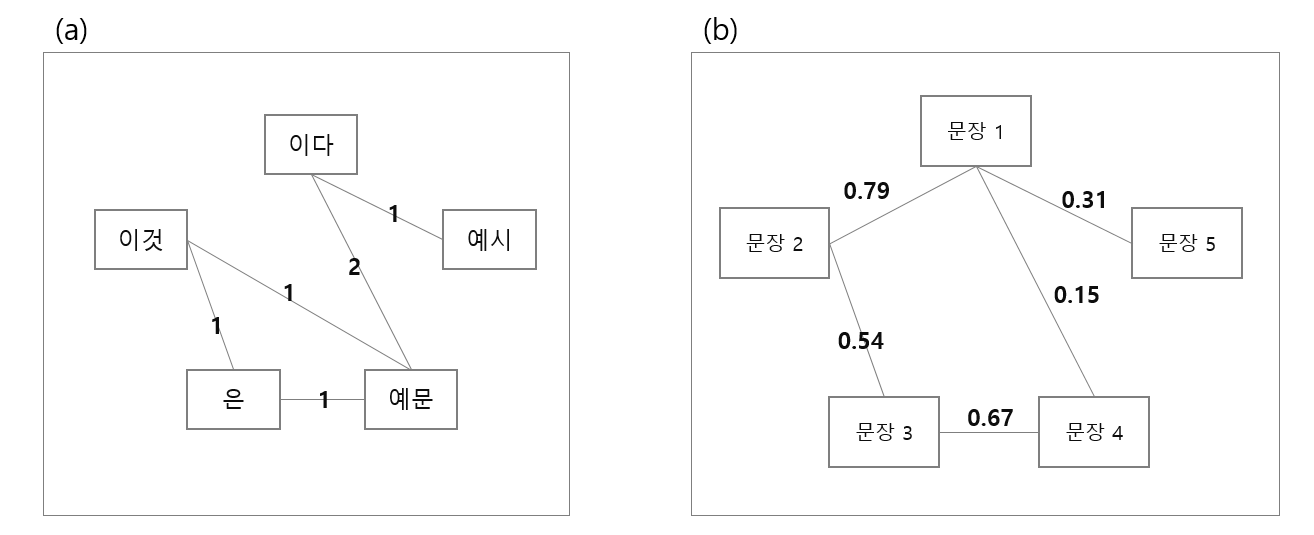
\includegraphics[keepaspectratio=true, width=0.9\linewidth]{figures/keyword_textrank.png}
\caption{(a) TextRank 의 co-occurrence 를 이용한 단어 그래프 예시, (b) TextRank 의 문장 간 유사도를 이용한 문장 그래프 예시}
\label{fig:textrank}
\end{figure}

셋째, PageRank \citep{ilprints422} 를 이용하여 단어 그래프 내의 각 마디의 랭크를 계산한다.
PageRank 의 식 \ref{eq:pagerank2} 에서는 모든 호의 가중치가 동일하지만, 그림 \ref{fig:textrank} (a) 에서는 호마다 가중치가 다르다.
그렇기 때문에 식 \ref{eq:textrank_pagerank} 처럼 한 마디에서 다른 마디로 이동하는 가중치의 합이 1 이 되도록 정규화 한 가중치를 이용하여 랭크를 계산한다.
빈도수가 높은 단어는 다른 단어들과 함께 등장한 빈도가 높기 때문에 연결된 마디의 가중치의 합이 크다.
그렇기 때문에 TextRank 는 문서 집합 내에서 빈도수가 높은 단어에 높은 랭크를 부여한다.
하지만 빈도수가 조금 작더라도 랭크가 높은 다른 단어들과 같은 문장에서 자주 등장하는 단어의 랭크도 높아진다.

\begin{equation}
\label{eq:textrank_pagerank}
PR(u) = c \times \sum_{v \in v \rightarrow u} \frac{w_{vu}}{\sum_{w \in v \rightarrow w} w_{vw}} PR(v) + (1-c) \times \frac{1}{N}
\end{equation}

문법 기능을 수행하는 조사나 어미는 다른 단어들보다 상대적으로 빈번하게 출연하기 때문에 (표 \ref{tab:pos_statistics}), 이들을 모두 단어 그래프에 포함하면 조사나 어미가 가장 높은 랭크를 가지게 학습된다.
그러므로 반드시 무의미한 단어를 제거한 뒤 단어 그래프를 생성해야 한다.

TextRank 의 키워드의 후보는 단어 그래프를 구성하는 모든 단어들이기 때문에 토크나이저가 중요한 단어를 정확히 인식하지 않으면 그 단어는 키워드가 될 수 없다.
특히 소셜미디어나 영화평과 같은 데이터에서는 고유명사가 미등록단어인 문제가 빈번하며 이들이 키워드일 가능성이 높다.
그러므로 TextRank 를 이용하여 키워드를 추출할 때에는 단어 사전을 반드시 보강해야 한다.

WordRank \citep{chen2011simple} 는 이러한 문제를 해결할 수 있는 방법이다.
WordRank 는 중국어와 일본어처럼 띄어쓰기가 이뤄지지 않은 언어에서 그래프 랭킹을 기반으로 단어를 추출하는 방법으로, 문장 내 가능한 모든 부분단어를 생성한 뒤, 인접한 부분단어의 빈도수를 기반으로 부분단어 그래프를 만든다.
WordRank 는 "부분단어 그래프에서는 단어와 연결된 마디가 단어이며, 잘못된 부분단어와 연결된 마디는 잘못된 부분단어"라는 가정을 바탕으로 단어를 추출한다.
그림 \ref{fig:keyword_krwordrank_assumption} (a) 처럼 단어나 어절의 앞 뒤에는 다른 단어나 어절이 등장하며, 그 종류가 다양하다.
하지만 그림 \ref{fig:keyword_krwordrank_assumption} (b) 처럼 단어가 아닌 부분단어의 앞 뒤에는 소수의 부분 단어들이 등장한다.
그렇기 때문에 부분단어 그래프에 PageRank 를 적용하면 단어인 마디들의 랭크가 높게 계산된다.
부분단어 그래프는 TextRank 가 이용하는 단어 그래프와 같은 구조이기 때문에 단어를 추출함과 동시에 키워드를 추출하는 능력이 있다.

\begin{figure}[H]
\centering
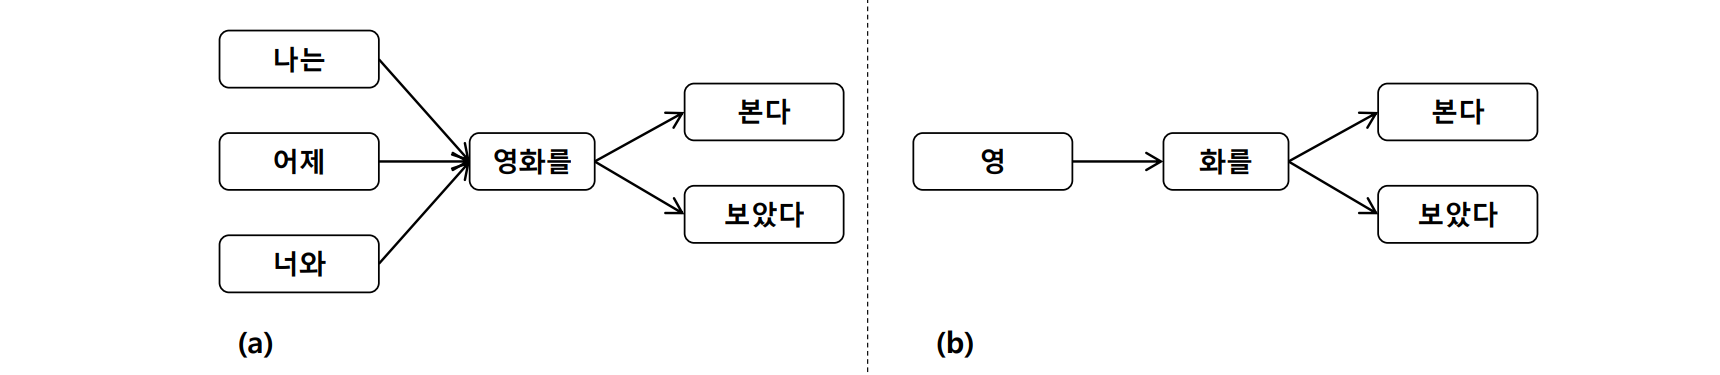
\includegraphics[keepaspectratio=true, width=0.9\linewidth]{figures/keyword_krwordrank_assumption.png}
\caption{(a) 어절을 마디로 이용하면 두 어절은 서로 이웃하며, (b) 잘못된 어절을 마디로 이용하면 잘못된 어절끼리 이웃한다.}
\label{fig:keyword_krwordrank_assumption}
\end{figure}

그러나 WordRank 를 한국어 데이터에 적용하면 다음과 같은 문제가 발생한다.
첫째, 옳지 않은 글자가 단어로 추출될 수 있다.
아래의 그림 \ref{fig:krwordrank_candidates} 는 WordRank 의 1 음절부터 3 음절까지의 단어후보이다.
첫 문장에서는 두 어절에 걸쳐진 '의날씨'는 단어 후보가 되어서는 안되지만, WordRank 는 이 글자를 단어 후보로 선택한다.
만약 다른 문장에서도 두 어절에 걸쳐 '의날씨'라는 글자가 자주 등장한다면 WordRank 는 '의날씨'를 핵심 단어로 선택한다.

\begin{figure}
\label{fig:krwordrank_candidates}
\begin{itemize}[noitemsep]
  \item 문장 : '오늘의 날씨는 좋습니다', '내일의 날씨도 좋습니다'
  \item WordRank 단어 후보 : 오, 오늘, 오늘의, 늘, 늘의, 늘의날, 의, 의날, 의날씨, ...
  \item 한국어 단어 후보 : 오, 오늘, 오늘의, 날, 날씨, 날씨는, 좋, 좋습, 좋습니, 내, 내일, 내일의, ...
\end{itemize}
\end{figure}

둘째, 정보성이 적은 1음절 단어 혹은 형태소가 키워드로 추출된다.
조사는 그 종류가 적지만 대부분의 문장에서 등장하는 단어이며 이들은 대부분 길이가 1, 2 음절이다.
어미는 단어는 아니지만 용언의 말미에 반드시 등장하는 형태소이며, 이들의 종류는 다양하지만 실제 문장에는 몇몇 어미들이 매우 빈번히 등장한다.
이들은 문법 기능을 하는 단어 혹은 형태소로 의미를 지녀야하는 키워드로써는 부적합하다.
하지만 이들은 주요한 단어들의 앞 뒤에 등장하기 때문에 주요한 단어들과 co-occurrence 가 크다.

셋째, 키워드를 포함하는 어절이 중복되어 키워드로 추출된다.
예를 들어 영화 '아저씨'의 리뷰에는 배우 이름 '원빈' 이 자주 등장하며, 이 단어가 포함된 '원빈은', '원빈이', '원빈이다' 와 같은 어절들도 다수 존재한다.
WordRank 가 이용하는 부분글자 그래프는 '원빈'의 랭크가 계산되었을 때, '원빈은'의 랭크 값을 낮출 수 있는 구조가 이니기 때문에 '원빈'을 포함한 많은 글자들이 중복적으로 추출된다.

TextRank 를 이용한 핵심 문장 추출 과정은 다음의 과정으로 이뤄진다.
첫째, 토크나이저를 이용하여 문장을 단어열로 분해한다.
이 과정은 단어 그래프를 만드는 과정과 동일하다.

둘째, 각 문장을 그래프의 마디로, 두 문장 간 유사도를 마디 간 가중치로 정의한다.
TextRank 는 식 \ref{eq:textrank_sim} 과 같은 문장 간 유사도를 이용한다.

\begin{equation}
\label{eq:textrank_sim}
sim(s_1, s_2) = \frac{\vert \{ w_k \vert w_k \in S_1 \& w_k \in S_2 \} \vert}{log \vert S_1 \vert + log \vert S_2 \vert}
\end{equation}

셋째, PageRank \citep{ilprints422} 를 이용하여 문장 그래프 내의 각 마디의 랭크를 계산한다.
랭크가 높은 상위 $k$ 개의 문장을 핵심 문장으로 선택한다.

식 \ref{eq:textrank_sim} 은 두 문장에 공통으로 등장하는 단어의 개수를 두 문장의 길이의 로그값의 합으로 나눈 것으로, 문장의 길이가 길어질수록 분모의 증가분이 줄어들기 때문에 긴 문장에 큰 가중치를 부여하는 경향이 있다.
또한 빈번한 단어로 구성된 문장일수록 분자가 큰 경향이 있다.
그러므로 TextRank 는 문서 집합 전체에서 자주 등장하는 단어들로 구성된 문장을 핵심 문장으로 선택한다.
이후 BM25 \citep{robertson2009probabilistic} 를 문장 간 유사도 함수로 이용하거나 \citep{barrios2016variations}, 코싸인 유사도를 이용하는 LexRank \citep{erkan2004lexrank} 가 제안되었다.

하지만 TextRank 를 이용하여 핵심 문장을 추출할 때에는 두 가지 문제가 발생한다.
첫째, 토크나이저가 단어를 제대로 인식하지 않으면 문장 간 유사도가 정확하게 계산되지 않는다.

둘째, 선택된 핵심 문장 간의 다양성이 보장되지 않는다.
TextRank 에서 형태가 매우 유사한 두 문장 중 하나의 문장의 랭크가 높다면 다른 문장도 랭크가 높으며, 상위 $k$ 개의 문장을 선택하는 과정에서 중복된 문장이 선택될 가능성이 있다.
중복적인 핵심 문장은 정보력이 적기 때문에, 핵심 문장은 다양한 내용으로 구성되어야 한다.

이를 해결하기 위하여 핵심 문장 간의 다양성을 유도하는 연구도 제안되었다 \citep{mcdonald2007study, parveen2015topical}.
핵심 문장의 품질을 목적식으로 정의하면 주어진 문장에서 핵심 문장을 선택하는 문제는 정수 최적화 문제로 정의할 수 있다.
목적식에 선택된 핵심 문장들이 중복적일 경우 그 값이 적어지는 항목을 추가하거나 핵심 문장들이 서로 비슷하지 않도록 제약식을 추가할 수 있다.


%%%%%%%%%%%%%%%%%%%%%%%%%%%%%%%%%%%%%%%%%%%%%%%%%
\subsection{제안하는 방법: KR-WordRank}

\subsubsection{토크나이저를 이용하지 않는 한국어 키워드 추출 방법}

kR-WordRank 는 위 세가지 문제를 해결하기 위하여 제안된 그래프 랭킹 기반 한국어 키워드 추출 방법으로, 주어진 데이터로부터 직접 단어를 추출하는 능력이 있기 때문에 미등록단어 문제에서 자유롭다 \citep{kim2014kr}.

KR-WordRank 는 다음과 같은 과정으로 학습된다 (그림 \ref{fig:krwordrank_framework}).
첫째, 문장을 어절 단위로 분해하여 빈도수를 계산한다.

둘째, \ref{lrstructure} 장에서 제안한 L + [R] 구조를 이용하여 각 어절에서 L 과 R 에 해당하는 부분어절의 빈도를 계산한다.
띄어쓰기 오류가 존재한다 하여도 잘못 추출된 L 과 R 의 빈도수는 상대적으로 작기 때문에 이들이 키워드로 선택될 가능성은 적다.

셋째, L 과 R 별로 빈도수가 같으며, 한 부분어절에 포함되는 짧은 부분어절을 제거한다.
그림 \ref{fig:krwordrank_framework} 에서 '원/L' 과 '원빈/L' 이 모두 2 번 등장하였기 때문에 '원/L' 은 '원빈/L' 을 반드시 지칭하기 때문이다.

넷째, 어절 간에는 부분어절 L 과 L 사이에, 어절 내에는 부분어절 L 과 R 사이의 빈도수를 두 마디 간 가중치로 정의한다.
이 과정을 통하여 앞선 예제의 '은하'는 그래프의 마디에서 제외된다.

다섯째, PageRank 를 이용하여 마디의 랭크를 계산한다.
랭크는 단어 가능성 점수임과 동시에 키워드 점수이다.

\begin{figure}[H]
\centering
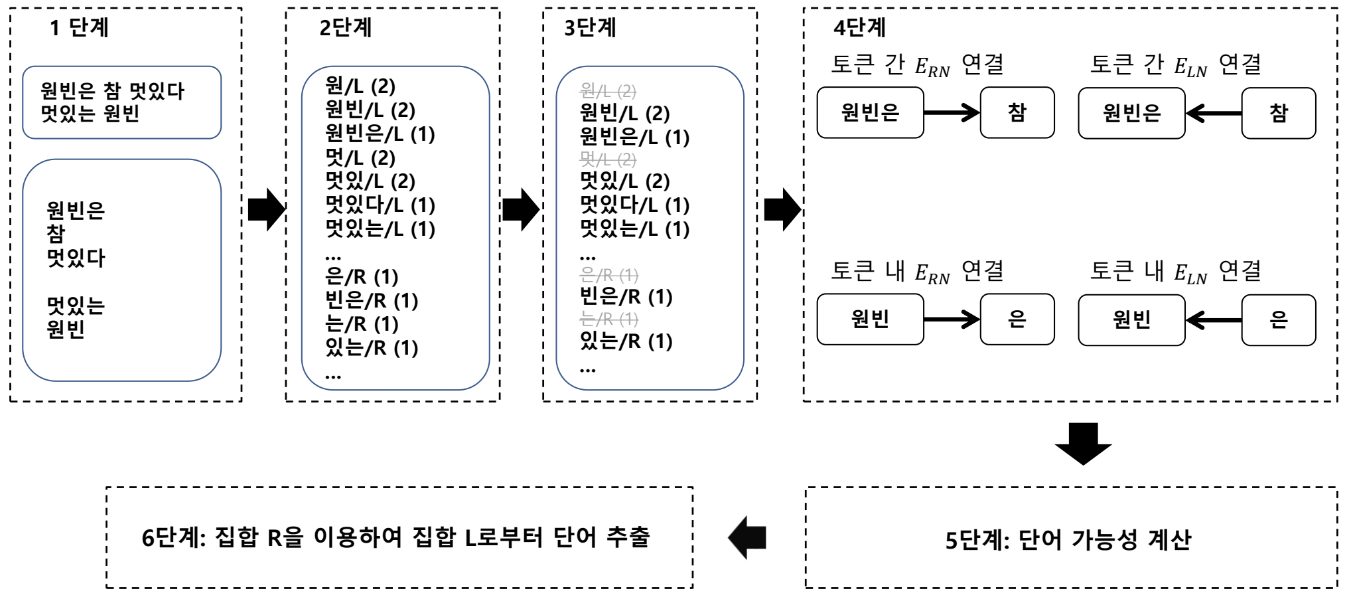
\includegraphics[keepaspectratio=true, width=0.9\linewidth]{figures/krwordrank_framework.png}
\caption{KR-WordRank 의 키워드 추출 프레임워크}
\label{fig:krwordrank_framework}
\end{figure}

여섯째, 필터링 과정을 거쳐 L + R 형태의 키워드를 제거한다.
부분어절 R 중 랭킹이 높은 순으로 $r_k$ 개의 부분어절을 선택한다.
이는 이 도메인에서 이용되는 조사 혹은 어미 집합이며, 키워드는 부분어절 L 에서만 선택한다.
부분어절 L 중 랭킹이 높은 순으로 정렬한 뒤, 랭킹이 낮은 $l$ 이 이미 선택된 키워듸 $w$ 와$[r_1, \dots r_{r_k}]$ 의 조합이 아니면 키워드 집합에 추가한다 (그림 \ref{fig:krwordrank_filtering}).
위의 예시에서 '원빈'이 키워드로 선택되면 '원빈 + [이, 은, 이다]' 는 키워드로 선택되지 않는다.

\begin{figure}[H]
\renewcommand{\arraystretch}{0.7}
\centering
\begin{tabular}{|l|}
\hline
\begin{tabular}[c]{@{}l@{}}
$L = [l_1, l_2, \dots, l_L]$ : L 에 해당하는 마디 집합 \\
$R = [r_1, r_2, \dots, r_k]$ : L 에 해당하는 마디 집합 \\
\\
\textbf{def select\_keywords}($L, R_k$): \\
\quad $KW$ = { } : 키워드 집합 \\
\quad \textbf{For} $c$ in $L$: \\
\quad \quad if $c$ is not form of $kw_{i} + r_j$: \\
\quad \quad \quad $KW \leftarrow KW \cup {c}$ \\
\quad \textbf{return} $KW$ \\
\end{tabular} \\ \hline
\end{tabular}
\caption{KR-WordRank 키워드 필터링 함수}
\label{fig:krwordrank_filtering}
\end{figure}

\subsubsection{키워드 집합을 이용한 핵심 문장 선택}

한 문서 집합을 대표하는 핵심 문장은 그 집합의 키워드를 다수 포함해야 한다.
TextRank 는 문서 집합 전체에서 자주 등장하는 단어들로 구성된 문장을 핵심 문장으로 선택하며 길이가 긴 문장을 선호하는 경향이 있기 때문에 키워드가 포함될 가능성이 높다.
그러나 핵심 문장들 간의 다양성은 보장되지 않으며, 토크나이징 결과를 이용하여 문장 간 유사도를 계산한다.

이 장에서는 앞서 제안한 키워드 추출 방법을 이용하여 핵심 문장을 추출하는 방법을 제안한다 (그림 \ref{fig:krwordrank_framework_sentence}).

\begin{figure}[H]
\centering
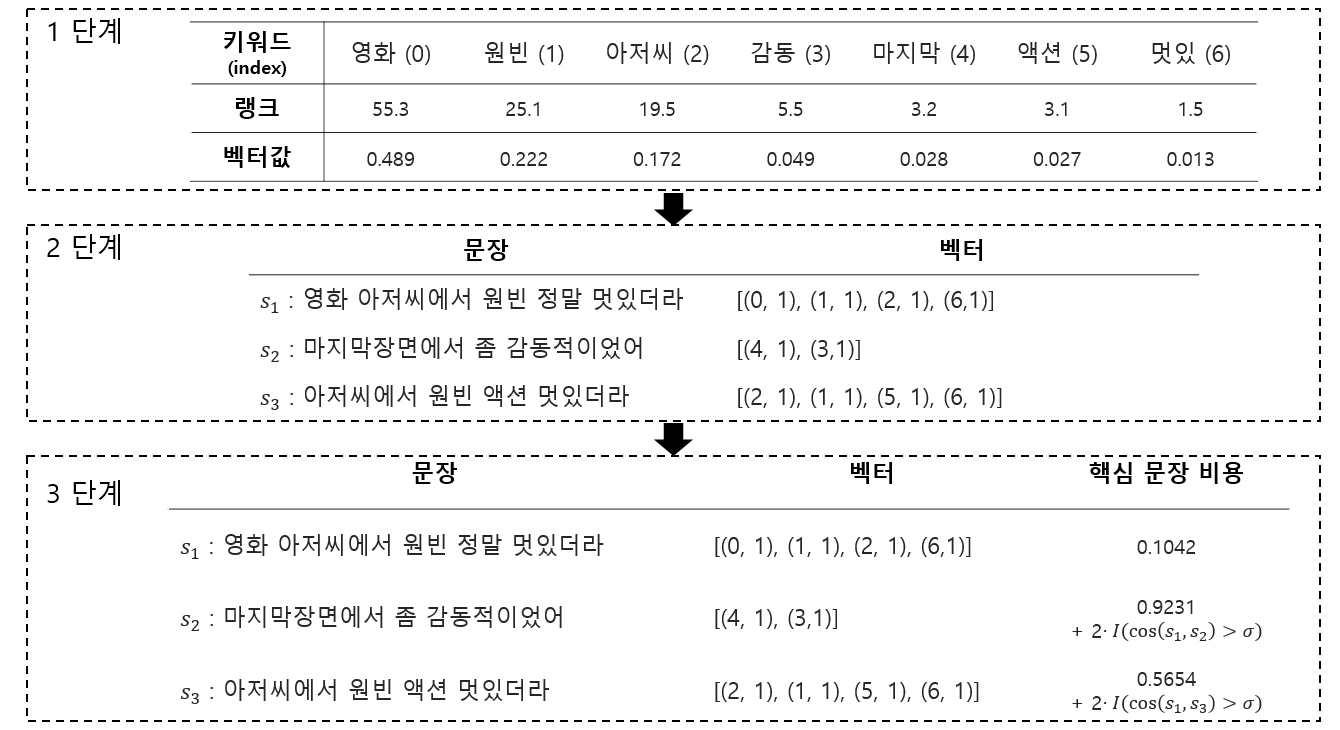
\includegraphics[keepaspectratio=true, width=0.9\linewidth]{figures/krwordrank_framework_sentence.png}
\label{fig:krwordrank_framework_sentence}
\caption{KR-WordRank 의 핵심 문장 추출 프레임워크}
\end{figure}

첫 단계에서 키워드 추출을 통하여 학습한 랭크를 벡터로 변환한다.
PageRank 를 이용하여 학습한 랭크 값은 지수 분포를 따르는 경향이 있는데, 순위가 낮은 키워드의 랭크를 상대적으로 높이기 위해서 랭크의 1/2 승을 취할 수도 있다.
이를 키워드 벡터 ($KV$) 라 명한다.

두번째 단계에서는 \ref{word_extraction} 장에서 제안한 Max Score Tokenizer 를 이용하여 각 문장을 키워드의 포함 유무 벡터로 표현한다.
키워드의 랭크를 단어 점수로 이용하면 문장에서 키워드를 우선적으로 단어로 분리한다.

세번째 단계에서는 각 문장 벡터와 키워드 벡터의 유사도를 이용하여 키워드가 많이 포함된 문장을 핵심 문장으로 선택한다 (그림 \ref{fig:krwordrank_sentence_filtering}).
키워드들이 다수 포함된 문장이라면 문서 집합을 대표할 가능성이 높기 때문이다.
이를 위하여 키워드 벡터 $KV$ 와 문장 간의 코싸인 거리를 계산하여 이를 핵심 문장 비용으로 정의한 뒤, 핵심 문장 비용이 가장 적은 문장 $S_i$ 를 첫번째 핵심 문장으로 선정한다.
그 뒤 문장 $S_i$ 와 다른 문장 간의 거리가 $\sigma$ 보다 작은 문장들에 페널티 비용을 추가한다.
이후 핵심 문장 리스트 $KS$ 의 크기가 $k$ 가 되기 전까지 비용이 가장 작은 문장을 선택하는 과정을 반복한다.
이 과정은 제안한 방법이 키워드를 다수 포함한 문장들 중에서 서로 이질적인 문장을 핵심 문장으로 선택하도록 유도한다.

\begin{figure}[H]
\renewcommand{\arraystretch}{0.7}
\centering
\begin{tabular}{|l|}
\hline
\begin{tabular}[c]{@{}l@{}}
$KV$ : 랭크로 이뤄진 키워드 벡터 \\
$S$ : Max Score Tokenizer 와 키워드 랭크를 이용하여 벡터화 된 문장\\
\\
\textbf{def select\_keysentences}($S, KV, \sigma, k$): \\
\quad $\sigma$ : 사용자에 의하여 지정된 핵심 문장간 최소 거리 \\
\quad $k$ : 핵심 문장 개수
\quad $KS$ = [ ] : 핵심 문장 리스트 \\
\quad $C$ = $dist$($KV, S$) : 핵심 문장 비용\\
\quad \textbf{While} $\vert KS \vert < k$: \\
\quad \quad $i \leftarrow \arg \min_C$ \\
\quad \quad $KS \leftarrow KS + [S_i]$ \\
\quad \quad $C \leftarrow C + I(dist(S, S_i) < \sigma)$
\quad \textbf{return} $KS$
\end{tabular} \\ \hline
\end{tabular}
\caption{KR-WordRank 핵심 문장 필터링 함수}
\label{fig:krwordrank_sentence_filtering}
\end{figure}



%%%%%%%%%%%%%%%%%%%%%%%%%%%%%%%%%%%%%%%%%%%%%%%%%
\subsection{성능 평가}

제안하는 방법은 토크나이저를 이용하지 않는 키워드 추출과 이를 이용한 핵심 문장 추출로 이뤄져 있기 때문에 각 과업에 대한 성능을 각각 측정하였다.

제안하는 키워드 추출 방법의 단어 추출 능력을 평가하기 위하여 세종 말뭉치와 영화평 데이터를 이용하였다.
세종 말뭉치는 문장을 구성하는 형태소가 태깅되어 있기 때문에 단어 추출 능력에 대한 정량적인 평가가 가능하다.
제안하는 방법은 \ref{lrstructure} 장의 L + [R] 구조를 가정하기 때문에 세종 말뭉치의 어절을 L + [R] 구조로 변형하였다.
키워드는 해석이 가능한 독립언이기 때문에 체언과 용언의 표현형, 관형사, 부사, 감탄사를 정답 단어 집합으로 이용하였다.
WordRank, 1음절을 제외한 부분단어로 이뤄진 WordRank, 그리고 $R_k$ 의 크기를 300, 400, 500 으로 설정한 KR-WordRank 의 단어 인식 능력을 평가하였다 (그림 \ref{fig:krwordrank_performance}).
세종 말뭉치에 등장한 단어의 재현율을 정확도로 이용하였다.
그 결과 WordRank 에서는 20 \% 가 되지 않는 단어 인식 능력을 보이지만, 제안하는 방법은 $R$ 크기의 설정에 따라 70 \% 정도의 단어 인식 능력을 보였다.

\begin{figure}[H]
\centering
\label{fig:krwordrank_performance}
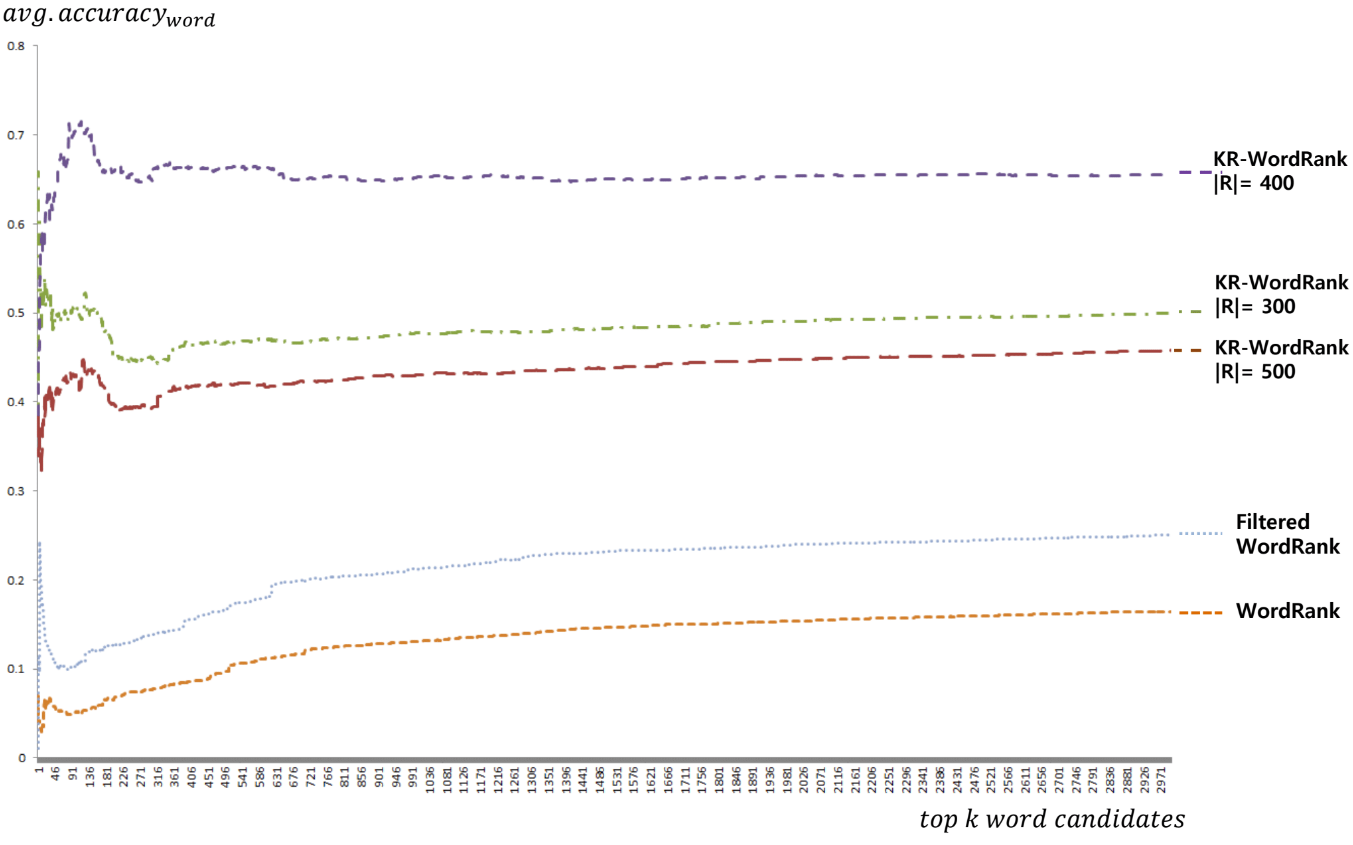
\includegraphics[keepaspectratio=true, width=0.9\linewidth]{figures/krwordrank_performance.png}
\caption{WordRank 와 KR-WordRank 를 이용하여 세종 말뭉치로부터 추출한 단어의 정확도}
\end{figure}

이는 \ref{noun_extraction} 장에서 제안한 명사 추출기의 재현율과 비교하면 매우 낮은 수치인데, 비교 실험에 이용한 WordRank 와 KR-WordRank 는 문서 집합의 주제가 단일할 때 좋은 성능을 보이기 때문이다.
그러나 세종 말뭉치는 여러 주제의 문서들이 모여있는 말뭉치이기 때문에 다양한 문서에서 상대적으로 많이 등장하는 단어들만 제대로 인식된다.
그렇기 때문에 영화 "아저씨"의 영화평에서 WordRank 와 KR-WordRank 를 이용하여 키워드를 출한 결과를 정성적으로 평가하였다 (그림 \ref{fig:krwordrank_vs_wordrank}).
문제 종류 A 는 해석이 불가능하거나 단어가 아닌 경우, B 는 조사나 어미가 결합된 어절, C 는 조사나 어미가 단어로 추출된 경우, D 는 복합명사인 경우이다.
문서 집합의 주제가 단일하더라도 WordRank 는 해석이 불가능한 1 음절을 키워드로 선택하는 경우가 많으며, 이는 대부분 조사나 어미로 추정된다.
WordRank 가 추출한 2 음절 이상의 키워드에는 '원빈의'와 같이 키워드와 조사가 결합된 경우와 2 음절 이상의 조사나 어미가 키워드로 추출된 경우가 많았다.
하지만 KR-WordRank 는 영화 '아저씨'를 대표하는 키워드들이 잘 추출되었으며, '한국영화'처럼 영화 도메인에서 자주 이용되는 복합명사도 키워드로 추출됨을 확인할 수 있다.
즉 제안하는 방법은 단일한 주제의 문서로 이뤄진 문서 집합을 대표하는 키워드를 추출할 수 있다.

\begin{figure}[H]
\centering
\label{fig:krwordrank_vs_wordrank}
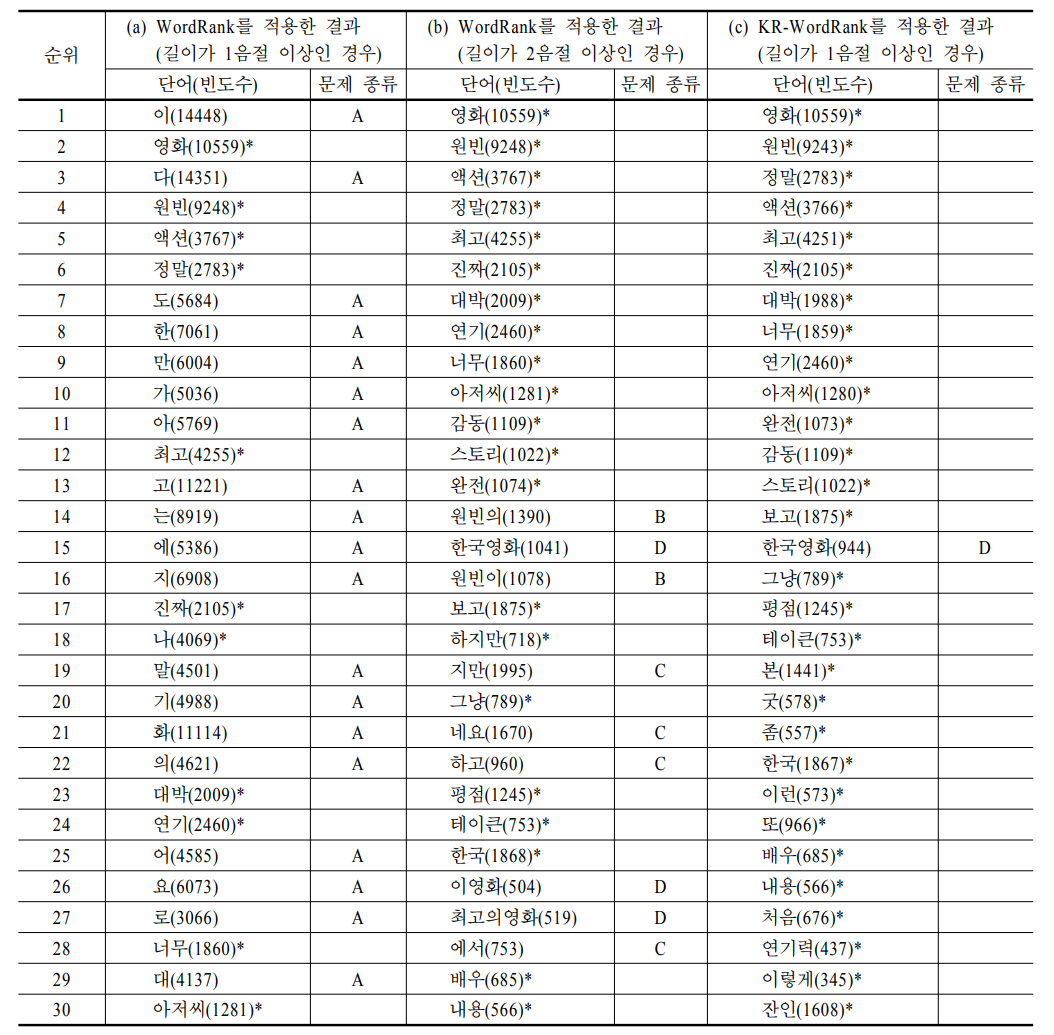
\includegraphics[keepaspectratio=true, width=0.9\linewidth]{figures/krwordrank_vs_wordrank.png}
\caption{WordRank 와 KR-WordRank 를 이용하여 추출한 영화 "아저씨" 리뷰의 키워드}
\end{figure}

제안하는 방법 핵심 문장 추출 능력을 평가하기 위하여 영화평 데이터에서 핵심 문장을 추출한 뒤, ROUGE-N \citep{lin2004rouge} 를 이용하여 문서 요약 능력을 평가하였다.
ROUGE-N 은 핵심 문장에 정답 문장의 n-gram 의 재현율로, 정답 문장에 포함된 단어가 많이 포함된 문장일수록 좋은 요약문으로 평가한다.
그러나 각 영화평마다 정답 요약 문장을 만드는 과정에는 주관이 개입될 수 있으며, 다른 평가 데이터를 이용할 때마다 정답 데이터를 만들어야 하기 때문에 확장 가능한 방법이 아니다.

제안하는 핵심 문장 추출 방법은 TextRank 가 중복된 문장들을 핵심 문장으로 선택하는 문제를 해결하기 위한 방법이기 때문에, 제안하는 방법에 의하여 선택된 핵심 문장들이 실제로 다양한 키워드를 포함하는지 확인하였다.
이를 위하여 네이버 영화로부터 각 영화의 영화평이 5000 개 이상 기록된 152 개의 영화로부터 약 320 만개의 영화평을 수집하였다.
특히 영화평 데이터에는 중복되거나 비슷한 문장이 다수 존재하기 때문에, 다양한 문장으로 핵심 문장을 구성하는 능력을 평가하기에 적합하다.
각 영화마다 TextRank 와 코싸인 유사도를 문장 유사도로 이용하는 LexRank, 그리고 제안하는 방법 (KR-WordRank) 을 이용하여 키워드와 핵심 문장을 추출하였다.
제안하는 방법의 사용자 정의 패러메터인 $\sigma$ 는 0.5 로 설정하였으며, TextRank 와 LexRank 는 코모란 토크나이저를 이용하여 형태소 분석을 수행하였다.
키워드 집합을 정답 문장으로 가정한 뒤, 핵심 문장들이 실제로 다양한 키워드를 포함하고 있는지를 확인하였다.
키워드는 하나의 단어로 구성되어 있기 때문에 ROUGE-1 을 이용하였다.

그 결과 제안하는 방법은 키워드와 핵심 문장의 개수에 상관없이 언제나 TextRank 나 LexRank 보다 더 높은 ROUGE-1 점수를 보였다.
또한 키워드 개수를 고정할 경우 핵심 문장의 개수가 늘어남에 따라 점수도 함께 증가하는데, 이는 제안하는 방법은 새로운 핵심 문장을 추가할 때마다 이전에 선택된 핵심 문장과 다른 문장들을 추가함을 의미한다.
코싸인 거리를 이용하는 LexRank 는 상대적으로 매우 낮은 성능을 보이는데, 이는 코싸인 척도는 길이가 매우 짧은 문장에 대하여 아주 큰 문장 간 유사도를 부여할 수 있기 때문에 1, 2 단어로 이뤄진 문장들이 핵심 문장으로 선택되었기 때문이다.
반면 TextRank 는 길이가 긴 문장을 선호하기 때문에 LexRank 보다 더 높은 키워드의 재현율을 보였다.

\begin{table}[H]
\centering
\small
\label{tab:krwordrank_sentence_performance}
\caption{제안하는 방법 (KR-WordRank), TextRank, 그리고 LexRank 로부터 추출된 핵심 문장의 ROUGE-1 성능. 각 알고리즘이 추출한 키워드를 정답 문장으로 이용}
\begin{tabular}{|c|c|c|c|c|}
\hline
\textbf{\# keywords} & \textbf{\# keysents} & \textbf{KR-WordRank} & \textbf{TextRank} & \textbf{LexRank} \\ \hline
10 & 3 & 0.942 & 0.752 & 0.156 \\ \hline
10 & 5 & 0.983 & 0.81 & 0.166 \\ \hline
10 & 10 & 0.998 & 0.855 & 0.197 \\ \hline
10 & 20 & 1 & 0.904 & 0.244 \\ \hline
10 & 30 & 1 & 0.92 & 0.291 \\ \hline
20 & 3 & 0.758 & 0.603 & 0.078 \\ \hline
20 & 5 & 0.873 & 0.69 & 0.084 \\ \hline
20 & 10 & 0.966 & 0.767 & 0.101 \\ \hline
20 & 20 & 0.994 & 0.839 & 0.135 \\ \hline
20 & 30 & 0.998 & 0.869 & 0.17 \\ \hline
30 & 3 & 0.631 & 0.496 & 0.053 \\ \hline
30 & 5 & 0.771 & 0.587 & 0.056 \\ \hline
30 & 10 & 0.911 & 0.688 & 0.069 \\ \hline
30 & 20 & 0.98 & 0.778 & 0.093 \\ \hline
30 & 30 & 0.994 & 0.82 & 0.12 \\ \hline
50 & 3 & 0.48 & 0.363 & 0.032 \\ \hline
50 & 5 & 0.621 & 0.452 & 0.034 \\ \hline
50 & 10 & 0.804 & 0.565 & 0.042 \\ \hline
50 & 20 & 0.929 & 0.674 & 0.058 \\ \hline
50 & 30 & 0.968 & 0.731 & 0.078 \\ \hline
\end{tabular}
\end{table}

아래는 각 방법에 의하여 '라라랜드'의 영화평에서 추출한 핵심 문장의 예시이다 (표 \ref{tab:krwordrank_sentence_example}).
제안한 방법과 TextRank 모두 해당 영화의 내용을 잘 대표하는 문장들이 핵심 문장으로 선택되었다.
이들은 표 \ref{tab:krwordrank_keyword_example} 의 키워드를 다수 포함하고 있다.
LexRank 의 경우 다른 방법론보다 짧은 문장이 핵심 문장으로 선택되었음을 확인할 수 있다.

\begin{table}[H]
\centering
\small
\caption{제안하는 방법 (KR-WordRank), TextRank, 그리고 LexRank 로부터 추출된 핵심 문장 예시}
\label{tab:krwordrank_sentence_example}
\begin{tabular}{|c|l|}
\hline
\textbf{추출 방법} & \multicolumn{1}{c|}{\textbf{핵심 문장}} \\ \hline
\multirow{4}{*}{\textbf{KR-WordRank}} & \begin{tabular}[c]{@{}l@{}}여운이 크게남는영화 엠마스톤 너무 사랑스럽고 라이언고슬링\\ 남자가봐도 정말 매력적인 배우인듯 영상미 음악 연기 구성 전부 좋았고\\ 마지막 엔딩까지 신선하면서 애틋하구요 30중반에 감정이 많이 메말라있었는데\\ 오랜만에 가슴이 촉촉해지네요\end{tabular} \\ \cline{2-2} 
 & \begin{tabular}[c]{@{}l@{}}영상미도 너무 아름답고 신나는 음악도 좋았다 \\마지막 세바스찬과 미아의 눈빛교환은 정말 마음 아팠음\\ 영화관에 고딩들이 엄청 많던데 고딩들은 영화 내용 이해를 못하더라ㅡㅡ\\ 사랑을 깊게 해본 사람이라면 누구나 느껴볼수있는 먹먹함이 있다\end{tabular} \\ \cline{2-2} 
 & \begin{tabular}[c]{@{}l@{}}정말 영상미랑 음악은 최고였다 그리고 신선했다\\ 음악이 너무 멋있어서 연기를 봐야 할지 노래를 들어야 할지 모를 정도로\\ 그리고 보고 나서 생각 좀 많아진 영화 정말 이 연말에 보기 좋은 영화 인 것 같다\end{tabular} \\ \cline{2-2} 
 & \begin{tabular}[c]{@{}l@{}}무언의 마지막 피아노연주 완전 슬픔ㅠ보는이들에게 꿈을 상기시켜줄듯\\ 또 보고 싶은 내생에 최고의 뮤지컬영화였음 단순할수 있는 내용에\\ 뮤지컬을 가미시켜째즈음악과 춤으로 지루할틈없이 빠져서봄 ost너무좋았음\end{tabular} \\ \hline
\multirow{4}{*}{\textbf{TextRank}} & \begin{tabular}[c]{@{}l@{}}처음엔 초딩들 보는 그냥 그런영화인줄 알았는데 정말로 눈과 귀가 즐거운 영화였습니다\\ 어찌보면 뻔한 스토리일지 몰라도 그냥 보고 듣는게 즐거운\\ 그러다가 정말 마지막엔 너무 아름답고 슬픈 음악이 되어버린\end{tabular} \\ \cline{2-2} 
 & 시사회 보고 왔어요 꿈과 사랑에 관한 이야기인데 뭔가 진한 여운이 남는 영화예요 \\ \cline{2-2} 
 & \begin{tabular}[c]{@{}l@{}}시사회 갔다왔어요 제가 라이언고슬링팬이라서 하는말이아니고 너무 재밌어요\\ 꿈과 현실이 잘 보여지는영화 사랑스런 영화 전 개봉하면 또 볼생각입니당\end{tabular} \\ \cline{2-2} 
 & 황홀하고 따뜻한 꿈이었어요 imax로 또 보려합니다 좋은 영화 시사해주셔서 감사해요 \\ \hline
\multirow{4}{*}{\textbf{LexRank}} & \begin{tabular}[c]{@{}l@{}}시사회에서 보고왔는데 여운쩔었다 엠마스톤과 라이언 고슬링의 케미가\\ 도입부의 강렬한음악좋았고 예고편에 나왓던 오디션 노래 감동적이어서 눈물나왔다ㅠ\\ 이영화는 위플래쉬처럼 꼭 영화관에봐야함 색감 노래 배우 환상적인 영화\end{tabular} \\ \cline{2-2} 
 & \begin{tabular}[c]{@{}l@{}}방금 시사회로 봤는데 인생영화 하나 또 탄생했네 롱테이크 촬영이 예술 영상이 넘나 아름답고\\ 라이언고슬링의 멋진 피아노 연주 엠마스톤과의 춤과 노래 눈과 귀가 호강한다\\ 재미를 기대하면 약간 실망할수도 있지만 충분히 훌륭한 영화\end{tabular} \\ \cline{2-2} 
 & 좋다 좋다 정말 너무 좋다 그 말 밖엔 인생영화 등극 ㅠㅠ \\ \cline{2-2} 
 & 음악도 좋고 다 좋고 좋고좋고 다 좋고 씁쓸한 결말 뭔가 아쉽다 \\ \hline
\end{tabular}
\end{table}

표 \ref{tab:krwordrank_keyword_example} 는 제안하는 방법과 TextRank 를 이용하여 추출한 키워드의 예시이다.
LexRank 와 TextRank 는 문장 간 유사도가 다른 방법이기 때문에 키워드는 TextRank 를 이용하여 추출한 결과만 확인한다.
제안하는 방법은 토크나이저를 이용하지 않으며 부분어절을 키워드로 선택하기 때문에 용언의 표현형의 일부를 단어로 선택한다.
그 결과 '재미'나 '재밌'처럼 원형은 같지만 표현형이 다른 두 부분단어가 모두 키워드로 선택되는 단점이 있다.
하지만 형태소 분석 과정을 거치지 않았음에도 불구하고 제안하는 방법에 의하여 선택된 키워드는 명사, 동사, 형용사, 부사와 같이 의미를 지니는 단어 혹은 부분단어가 선택되었다.

\begin{table}[H]
\centering
\small
\caption{제안하는 방법 (KR-WordRank), TextRank 을 이용하여 추출한 키워드 예시}
\label{tab:krwordrank_keyword_example}
\begin{tabular}{|c|c|c|c|}
\hline
\multicolumn{2}{|c|}{\textbf{KR-WordRank}} & \multicolumn{2}{c|}{\textbf{TextRank}} \\ \hline
영화 (201.34) & 현실 (15.21) & 영화/NNG (173.00) & 번/NNB (20.26) \\ \hline
너무 (81.80) & 생각 (14.94) & 보/VV (128.93) & 거/NNB (19.67) \\ \hline
정말 (40.62) & 지루 (13.81) & 좋/VA (65.55) & 최고/NNG (19.18) \\ \hline
음악 (40.52) & 다시 (13.62) & 하/VV (52.02) & 때/NNG (19.15) \\ \hline
마지막 (38.73) & 감동 (13.61) & 것/NNB (47.43) & 사람/NNG (19.04) \\ \hline
뮤지컬 (23.24) & 보는 (12.49) & 같/VA (45.37) & 여운/NNP (17.55) \\ \hline
최고 (21.85) & 좋아 (12.01) & 영화/NNP (43.89) & 뮤지컬/NNP (16.94) \\ \hline
사랑 (20.69) & 재밌 (11.91) & 음악/NNG (43.59) & 나오/VV (16.54) \\ \hline
꿈을 (20.47) & 재미 (11.41) & 꿈/NNG (41.43) & 듯/NNB (16.11) \\ \hline
아름 (20.36) & 좋고 (11.39) & 있/VV (40.79) & 영상미/NNG (15.95) \\ \hline
영상 (20.33) & 계속 (11.16) & 없/VA (35.94) & 지루/XR (15.66) \\ \hline
여운이 (19.51) & 조금 (10.95) & 마지막/NNG (31.92) & 처음/NNG (15.25) \\ \hline
진짜 (19.10) & 느낌 (10.94) & 수/NNB (30.08) & 장면/NNG (15.15) \\ \hline
노래 (18.77) & 처음 (10.76) & 사랑/NNG (28.25) & 감동/NNG (15.14) \\ \hline
보고 (18.60) & 결말 (10.60) & 아름답/VA (26.47) & 가/VV (15.03) \\ \hline
좋았 (17.66) & 연기 (10.52) & 현실/NNG (24.82) & 만들/VV (13.50) \\ \hline
그냥 (16.60) & 장면 (10.38) & 되/VV (23.91) & 들/VV (13.24) \\ \hline
스토리 (16.27) & 그리고 (10.36) & 노래/NNG (23.39) & 남/VV (13.21) \\ \hline
좋은 (15.67) & 하는 (10.28) & 생각/NNG (23.19) & 느낌/NNG (13.13) \\ \hline
인생 (15.41) & 있는 (10.17) & 스토리/NNP (21.35) & 말/NNG (13.13) \\ \hline
\end{tabular}
\end{table}


%%%%%%%%%%%%%%%%%%%%%%%%%%%%%%%%%%%%%%%%%%%%%%%%%
\subsection{결론}

이 장에서는 한국어의 문서 요약 과정에서 발생할 수 있는 미등록단어 문제를 해결하고 요약 문장의 다양성을 유도하는 추출 기반 문서 요약 방법을 제안하였다.
제안된 방법은 주제가 다양한 문서로 이뤄진 세종 말뭉치를 이용한 단어 인식 능력 평가에서 약 70 \% 에 가까운 단어 추출 정확도를 보였다.
주제가 단일한 영화평 데이터에 적용한 결과 토크나이저를 이용하지 않았음에도 의미를 지니는 단어들만을 키워드로 선택하였으며 문서 집합을 대표하며 단어를 키워드로 추출할 수 있음이 정성적으로 평가되었다.
또한 제안된 핵심 문장 추출 방법은 토크나이저를 이용하지 않았음에도 다양한 키워드를 포함한 문장들을 핵심 문장으로 선택할 수 있다.

그러나 제안된 방법은 몇 가지 한계점이 있다.
앞서 언급한 것처럼 제안한 방법은 음절 단위로 분리된 부분 단어 중에서 키워드를 선택하기 때문에 용언의 표현형이 서로 다른 부분어절을 모두 키워드로 선택할 가능성이 있으며, 중복된 단어가 많을수록 사용자가 느끼는 키워드의 품질은 낮아진다.
또한 핵심 문장에 띄어쓰기나 문법 오류가 포함되어 있다 하더라도 이를 교정하지 않기 때문에 비문들에 의하여 문서 집합이 요약될 수 있다.
문서 요약 과업은 그 결과를 사용자가 직접 보는 경우가 많기 때문에 이러한 오류를 교정하는 후처리 과정이 추가된다면 사용자의 만족도를 향상시킬 수 있다.


%%%%%%%%%%%%%%%%%%%%%%%%%%%%%%%%%%%%%%%%%%%%%%%%%%%%%%%%%%%%%%%%%%%%%%%%%%%%%%%
\newpage
\section{문서 군집화 알고리즘 및 군집화 레이블링을 이용한 다주제 문서 집합 요약} \label{improved_kmeans}

%%%%%%%%%%%%%%%%%%%%%%%%%%%%%%%%%%%%%%%%%%%%%%%%%
\subsection{개요}

문서 요약 과업은 하나의 문서를 요약하는 과업과 여러 개의 문서를 요약하는 과업으로 분류되지만, 여러 개의 문서가 단일한 주제의 문서로 구성되어 있다면 단일 문서의 요약 방법이 적용될 수 있다.
이 때는 \ref{summarize_single_topic} 장에서 제안한 것과 같은 그래프 랭킹 알고리즘을 기반으로 한 키워드나 핵심 문장 추출 방법이 주로 이용된다.
하지만 문서 집합에 여러 종류의 주제가 섞여있을 때에는 정보력이 적은 흔한 단어가 키워드로 선택된다 \citep{goldstein2000multi, lin2002single, filippova2008sentence, filippova2010multi}.

문서 집합이 여러 주제의 문서들로 구성되어 있을 때에는 문서 집합을 주제 별로 나눈 뒤, 각 주제 별로 문서를 요약할 수 있다.
이를 위하여 LDA \citep{blei2003latent} 와 같은 토픽 모델링을 통하여 주제를 학습 한 뒤 토픽 레이블링 기법 \citep{sievert2014ldavis} 을 이용하여 주제 별 키워드를 탐색하거나, 문서 군집화를 이용하여 문서 집합을 단일한 주제의 부분 집합으로 구분한 뒤, 각 군집별로 문서를 요약할 수 있다 \citep{wan2008multi, erkan2004lexpagerank, twinandilla2018multi}.

그러나 샘플링 기법을 기반으로 학습하는 LDA 는 문서 집합의 크기가 클 경우 많은 계산량이 필요하며 \citep{yuan2015lightlda}, 불용어제거와 같은 전처리 과정이 잘 이뤄지지 않으면 학습이 제대로 되지 않거나 불필요한 토픽과 단어들이 주요한 토픽과 단어로 해석되기도 한다 \citep{darling2011theoretical, newman2010evaluating}.
LDA 는 하나의 문서에 여러 개의 주제가 존재한다는 가정하지만 뉴스나 블로그와 같이 길지 않은 문서는 사실 하나의 주제를 가지는 경우가 많으며, 문서 군집화 역시 토픽 모델링으로 이용할 수 있다 \citep{dhillon2001concept, xu2003document, xie2013integrating}.

\ref{improved_kmeans} 장에서는 문서가 하나의 주제로 구성되어 있다고 가정할 때, 문서 군집화 기법을 이용하여 여러 주제로 구성된 문서 집합을 요약하기 위한 방법을 제안한다.
그러나 대량의 문서 요약을 위하여 k-means 군집화 기법과 키워드, 핵심 단어를 추출하는 과정에서는 비효율이 발생한다.
k-means 는 다른 알고리즘보다 빠른 학습 속도를 보여주지만 여전히 효율을 개선할 부분이 존재하며, 군집화 이후 각 군집마다 키워드나 핵심 문장을 추출하기 위한 방법을 적용하려면 추가적인 모델 학습이 필요하다.
\ref{improved_kmeans} 장에서는 효율적인 문서 군집화를 위하여 k-means 를 개선하며, 군집화 결과를 이용하여 추가적인 모델 학습 없이 군집 별 키워드를 추출하는 방법을 제안한다.

%%%%%%%%%%%%%%%%%%%%%%%%%%%%%%%%%%%%%%%%%%%%%%%%%
\subsection{관련 연구}

문서 군집화는 각 문서가 속한 집합에 대한 레이블이 없는 상황에서, 문서 간 유사성을 바탕으로 비슷한 문서를 묶는 비지도학습 기반 과업이다 \citep{xu2015comprehensive, yang2017towards, xie2016unsupervised}.
이를 위해서 다양한 군집화 알고리즘이 이용될 수 있다.
DBSCAN \citep{ester1996density}과 같은 밀도 기반 군집화 알고리즘, 계층 구조 기반 군집화 알고리즘 \citep{sibson1973slink}, 혹은 그래프 기반 군집화 알고리즘 \citep{clauset2004finding} 는 다양한 군집화 문제에 이용되었다.
하지만 이들의 계산 비용은 $O(n^2)$ 이상이기 때문에 대량의 군집화에 적합하지 않다.

반면 k-means 는 군집화 방법은 $O(n)$ 의 계산 비용으로 학습할 수 있기 때문에 대량의 문서 군집화에 효과적이다 \citep{coates2012learning, he2013k, jin2013density, coates2011analysis}.
k-means 는 k-partition 문제의 해법을 계산하는 근사 알고리즘으로, 데이터를 k 개의 부분 집합으로 나누었을 때 각 부분 집한 내의 점들 간의 분산이 최소화 되는 해를 탐색한다 \ref{eq:kpartition}.

\begin{equation}
\label{eq:kpartition}
\centering
arg min_C\sum_{i=1}^{k} \sum_{x \in C_i} \vert x - c_i \vert^2 = arg min_C \sum_{i=1}^{k} \vert C_i \vert Var(C_i)
\end{equation}

\begin{flushleft}
$C$ : cluster index\\
$C_i$ : cluster i\\
$c_i$ : the centroid of cluster i\\
$x$ : a vector of a data point\\
$k$ : a number of clusters\\
\end{flushleft}

\citep{lloyd1982least} 에서 제안된 k-means 는 빠른 계산 속도와 적은 메모리 사용, 분산 계산이 쉬운 구조적 특징 때문에 대량의 데이터 군집화에 널리 이용되고 있다.
k-means 는 그림 \ref{fig:lloyd_kmeans} 의 과정으로 학습된다.
초기 군집 대표값 (initial centroids) 를 선정한 뒤, 데이터의 모든 점을 가장 가까운 군집 대표값의 레이블로 할당한다.
각 군집에 속한 데이터의 평균을 새로운 군집 대표값으로 설정한 뒤, 위 과정을 모델이 수렴할 때까지 반복한다.

\begin{figure}[H]
\renewcommand{\arraystretch}{0.7}
\centering
\begin{tabular}{|l|}
\hline
\begin{tabular}[c]{@{}l@{}}
$D$: dataset\\
$k$: a number of clusters\\
\\
\textbf{def kmeans} ($D, k$):\\
\quad $C$ $\leftarrow$ Initialize $k$ centroids with random sampling\\
\quad $L$ $\leftarrow$ Assign all points to its closest centroid\\
\quad \textbf{while} (not converged):\\
\quad \quad $C$ $\leftarrow$ Update centroids by averaging assigned date points \\
\quad \quad $L$ $\leftarrow$ Reassign all the points to its closest centroid\\
\quad \textbf{return} $C$, $L$

\end{tabular} \\ \hline
\end{tabular}
\caption{Lloyd k-means}
\label{fig:lloyd_kmeans}
\end{figure}

문서 군집화에는 문서 간 거리 척도의 설정이 중요하다.
일반적으로 문서는 bag-of-words model 과 같은 고차원 스파스 벡터나 Doc2Vec 과 같은 고차원의 분산 표상 표현 (distributed representation) 으로 표현된다 \citep{le2014distributed, dai2015document}.
Bag-of-words model 로 표현되는 문서 간의 유사도는 두 문서에 공통으로 등장한 단어 정보가 중요하지만, 유컬리디언 거리는 이를 제대로 표현하지 못하기 때문에 코싸인 거리 혹은 자카드 거리와 같은 척도를 이용해야 한다 \citep{huang2008similarity}.
또한 문서가 분산 표상 표현으로 표현된다 하더라도 임베딩 공간에서 두 객체의 유사도는 코싸인 거리를 이용하는 것이 좋다 \citep{levy2015improving}.
유컬리디언 거리 대신 코싸인 거리를 이용하는 k-means 를 spherical k-means 라 하며 문서 군집화 과업에 이용된다 \citep{dhillon2002iterative, buchta2012spherical}.

그러나 k-means 는 여전히 개선될 여지가 있다.
k-means 는 초기의 군집 중심값이 잘 설정어야 안정적인 학습 결과를 얻을 수 있다 \citep{arthur2007k}.
그림 \ref{fig:initialization_good_bad} (a) 처럼 데이터의 전체 영역에 펼처진 형태로 초기 군집 중심값이 선택되면 빠르고 안정적인 수렴이 가능하지만, \ref{fig:initialization_good_bad} (b) 처럼 한 지역에서 초기 군집 중심값이 선택되면 불안정한 학습 결과를 보인다.

\begin{figure}[H]
\centering
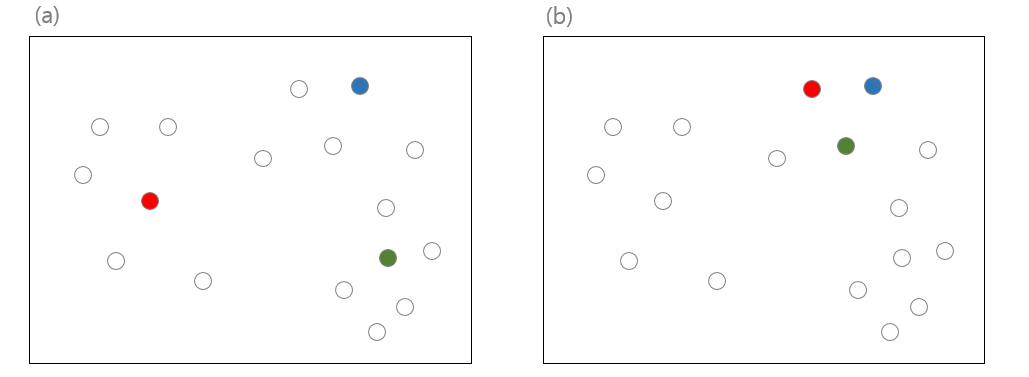
\includegraphics[keepaspectratio=true, width=0.95\linewidth]{figures/kmeans_initialization_good_bad.png}
\caption{(a) 기대하는 초기 군집 중심값, (b) 잘못된 초기 군집 중심값}
\label{fig:initialization_good_bad}
\end{figure}

이러한 초기화 문제를 해결하기 위하여 다양한 k-means 초기화 방법이 제안되었다.
Global k-means 는 순차적으로 초기 군집 중심값을 탐색하는 방법이다 \citep{likas2003global, bagirov2008modified}.
Global k-means 는 처음 데이터의 평균 벡터를 첫번째 군집의 초기값으로 이용한 뒤, 이 값을 고정한다.
그 뒤 임의로 새로운 한 점을 선택하여 $k=2$ 인 k-means 를 학습하여 두 개의 군집 중심값을 얻는다.
그 뒤 새로운 점을 추가하여 $k=3$ 인 k-means 를 학습한다.
이 과정을 군집의 개수가 $k$ 가 될때까지 반복한다.
그러나 이 과정은 $O(nk^2)$ 의 계산 비용을 요구하기 때문에 군집의 개수가 클 경우에는 매우 큰 학습 비용을 야기한다.

k-means++ \citep{arthur2007k} 은 이러한 문제를 해결한 k-means 초기화 알고리즘으로, 그림 \ref{fig:kmeanspp} 처럼 작동한다.
처음 한 점을 임의로 선택한 뒤, 다른 모든 점들 과의 거리 $d(x)$ 를 계산한다.
거리의 제곱을 정규화한 확률 분포를 기반으로 다른 한 점을 임으로 선택한다.
그 뒤 선택된 점들과 데이터의 모든 점들 간의 거리를 계산한 뒤, 선택된 점들 기준으로 가장 작은 거리값을 $d(x)$ 로 이용한다.
이 과정을 $k$ 개의 점이 선택되기 전까지 반복한다.
이 방법은 이미 군집 초기값으로 선택된 점과 그 주변의 점들이 선택될 확률을 작게 만듦으로써 데이터 전체에 펼쳐진 점들을 군집 초기값으로 선택한다.
그러나 이 방법 역시 여전히 $O(nk)$ 의 계산 비용이 요구된다.

\begin{figure}[H]
\centering
\begin{tabular}{|l|}
\hline
\begin{tabular}[c]{@{}l@{}}

1. Select point $c_1$ randomly \\
2. Select next point $c_t$ with probability $\frac{d(x)^2}{\sum_{x \in D} d(x)^2}$ \\
3. Repeat step 2 until $k$ points are chosen as initial points.\\

\end{tabular} \\ \hline
\end{tabular}
\caption{k-means++}
\label{fig:kmeanspp}
\end{figure}

또한 k-means++ 은 고차원 데이터에서 효율적으로 작동하지 않는다.
표 \ref{tab:cosine_distance_distribution} 는 실험에 이용한 7 종류의 고차원 데이터에서의 점들 간 코싸인 거리 분포이다.
고차원 공간에서는 대부분의 문서 간 코싸인 거리가 1 에 가깝기 때문에 그림 \citep{arthur2007k} 에서 계산된 확률 분포는 균등 분포에 가깝다.

\begin{table}[H]
\caption{고차원 벡터로 표현된 7 개의 텍스트 데이터에서의 코싸인 거리 분포. D1: A6 블로그, D2: 투스칸 블로그, D3: 소나타 블로그, D4: IMDb 리뷰, D5: Reuters RCV1, D6: MovieLens 20M, D7: Yelp 리뷰 데이터 (\%)}
\label{tab:cosine_distance_distribution}
\centering
%\resizebox{\textwidth}{!}{
\begin{tabular}{|c|c|c|c|c|c|c|c|}
\hline
\multirow{2}{*}{\textbf{Distance range}} & \multicolumn{7}{c|}{\textbf{Dataset}} \\ \cline{2-8} 
 & \textbf{D1} & \textbf{D2} & \textbf{D3} & \textbf{D4} & \textbf{D5} & \textbf{D6} & \textbf{D7} \\ \hline
\textbf{\textless{}= 0.7} & 0.249 & 0.59 & 0.323 & 0.272 & 0.045 & 1.456 & 0.01 \\ \hline
\textbf{0.7 - 0.8} & 0.378 & 1.121 & 0.455 & 7.751 & 0.067 & 2.386 & 0.286 \\ \hline
\textbf{0.8 - 0.9} & 1.628 & 3.89 & 1.984 & 57.271 & 0.316 & 12.458 & 11.073 \\ \hline
\textbf{0.9 - 1.0} & 97.745 & 94.399 & 97.239 & 34.706 & 99.573 & 83.7 & 88.632 \\ \hline
\end{tabular}
%}
\end{table}

%%%%%%%%%%%%%%%%%%%%%%%%%%%%%%%%%%%%%%%%%%%%%%%%%
\subsection{제안하는 방법: 문서 군집화를 위하여 개선된 Spherical k-means}

문서 군집화와 문서 요약을 위하여 개선된 spherical k-means 알고리즘은 두 가지 제안하는 방법이 추가되었다.
첫째, 코싸인 거리 척도를 이용하는 고차원 벡터 공간에서 효율적으로 작동하는 초기화 방법을 이용한다.
둘째, k-means 의 학습 결과인 군집 중심값을 이용하여 군집 별 키워드를 추출한다.

%%%%%%%%%%%%%%%%%%%%%%%%%%%%%%%%%%%%%%%%%%%%%%%%%
\subsubsection{문서 군집화를 위한 효율적인 Spherical k-means 초기화}

k-means 의 초기 군집 중심값이 그림 \ref{fig:initialization_good_bad} (b) 처럼 선택되면 불안정한 군집화 결과가 학습될 수 있다.
이를 개선하기 위하여 k-means++ 가 제안되었지만, $O(nk)$ 의 초기화 비용을 요구하며 고차원 벡터 공간에서는 효율적으로 작동하지 않는다.
고차원 벡터에서 서로 떨어진 초기 군집 중심값을 효율적으로 선택하기 위하여 그림 \ref{fig:proposed_initializer} 의 초기화 방법을 제안한다.

\begin{figure}[H]
\centering
%\resizebox{\textwidth}{!}{
\begin{tabular}{|l|}
\hline
\begin{tabular}[c]{@{}l@{}}

1. Construct set $D_{init}$, $\alpha \times k$ randomly selected data from data $D$\\
2. Select $c_i$ randomly from $D_{init}$\\
3. Remove $x_j$ where $x_j \in D_{init}$ and cos($⁡c_{i}, x_{j}$) $\ge t_{init}$\\
4. Repeat 2 $\sim$ 3 until $k$ centroid points are selected or $D_{init}$ becomes empty\\
5. If the number of selected centroid is less than $k$, then select\\ 
\quad remaining points from $D - D_{init}$ randomly\\

\end{tabular} \\ \hline
\end{tabular}
%}
\caption{개선된 Spherical k-means 초기화 방법}
\label{fig:proposed_initializer}
\end{figure}

제안하는 방법은 입력 데이터 $D$ 에서 군집의 개수 $k$ 의 $\alpha$ 배수의 점을 임의로 선택하여 $D_{init}$ 을 만든다.
$\alpha$ 는 사용자에 의하여 설정되는 패러메터이며, 실험을 통하여 1.5 에서 10 의 값이 적절함을 확인하였다.
제안하는 초기화 방법은 $D_{init}$ 에서 임의로 한 점을 선택한 뒤 $D_{init}$ 의 다른 점들과 코싸인 거리가 사용자 입력 패러매터인 $t_{init}$ 보다 작은 점들을 $D_{init}$ 에서 모두 제거한다.
그 뒤 다른 한 점을 $D_{init}$ 에서 임의로 선택한 뒤, 이를 $k$ 개의 점이 선택되거나 $D_{init}$ 이 공집합이 될 때 까지 반복한다.
만약 $k$ 개의 점을 선택하지 못한 경우에는 $D_{init}$ 에 속하지 않은 임의의 점을 선택하여 $k$ 개의 초기 군집 중심값을 선택한다. 

\begin{figure}[H]
\centering
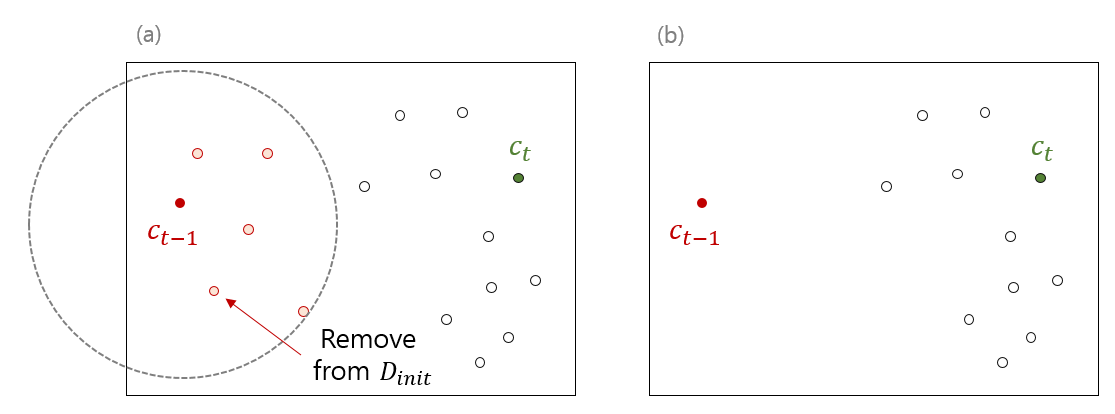
\includegraphics[keepaspectratio=true, width=0.95\linewidth]{figures/kmeans_initialization.png}
\label{fig:initialization}
\caption{개선된 Spherical k-means 초기화 방법의 예시 (a) 한 점이 선택된 뒤 코싸인 거리가 $t_{init}$ 보다 작은 점들을 제거한다 (b) 이후 임의의 한 점을 군집 초기값으로 선택한다}
\end{figure}

표 \ref{tab:cosine_distance_distribution} 에서 알 수 있듯이 대부분의 문서 간 코싸인 거리가 1 에 가깝기 때문에 $D_{init}$ 에서 임의의 점을 선택하여도 선택된 점들 간의 거리 역시 1 에 가까우며, 선택된 점들과 거리가 $t_{init}$ 보다 작은 점들을 제거하였기 때문에 한 지역에서 여러 개의 군집 초기값이 선택될 가능성은 매우 작다 (그림 \ref{fig:initialization}).
하지만 최대 $(\alpha \times k)^2$ 번의 거리 계산만 필요하기 때문에 문서 집합의 크기가 클 경우 적은 거리 계산만으로 군집 초기값을 선택할 수 있다 ($\alpha \times k \ll n$).


%%%%%%%%%%%%%%%%%%%%%%%%%%%%%%%%%%%%%%%%%%%%%%%%%
\subsubsection{중심 벡터를 이용한 문서 군집 별 키워드 추출 방법}

문서 군집화 과정은 각 문서가 속한 클래스의 정보가 존재하지 않는 상황에서 이용되기 때문에 군집 별 키워드에 대한 정답 데이터도 존재하지 않는 경우가 많다.
각 군집에 \ref{summarize_single_topic} 장에서 제안된 방법이나 TextRank 와 비지도학습 기반 문서 요약 방법을 적용할 수도 있으나, 이는 추가적인 모델 학습을 요구한다.
문서 군집화와 비슷한 분야인 토픽 모델링 분야에서도 비슷한 문제를 해결하기 위하여 비지도학습 기반 토픽 레이블링 기법이 활발히 연구되었다 \citep{newman2010evaluating, sievert2014ldavis, chuang2012interpretation, snyder2013topic, chuang2012termite, blei2003latent}.

문서 집합의 주제가 단일할 경우에는 빈도수가 높은 단어가 문서 집합을 대표하는 키워드일 가능성이 높다.
하지만 모든 군집에서 빈도수가 높은 단어는 정보를 지니지 않은 단어일 가능성이 높기 때문에 각 군집을 구분할 수 있는 단어를 군집의 키워드로 선택하는 것이 좋다.
그러나 군집 간 구분력이 좋은 단어는 빈도수가 작아 각 군집을 대표하지 못할 수 있다.
제안하는 군집 별 키워드 추출 방법은 군집 간 구분력과 군집의 대표성을 모두 고려하여 키워드를 추출한다.

식 \ref{eq:proposed_labeler} 은 제안하는 군집 별 키워드 추출 방법으로, $s(w, C_i$ 은 군집 $C_i$ 에서의 단어 $w$ 의 군집 구분력 점수이다.
$p_i (w)$ 는 군집 $C_i$ 에서의 단어 $w$ 의 등장 비율이며, $p_{-i} (w)$ 는 군집 $C_i$ 을 제외한 다른 문서 집합에서의 단어 $w$ 의 등장 비율이다.
$p_i (w)$ 와 $p_{-i} (w)$ 가 비슷하면 단어 $w$ 는 군집과 상관성이 적은 단어임을 의미하며, $p_i (w)$ 가 $p_{-i} (w)$ 보다 클 경우에는 군집 $C_i$ 에 유독 등장한 단어임을 의미한다.
$s(w, C_i)$ 의 범위는 [0, 1] 로 1 에 가까울수록 군집 $C_i$ 구분하는 단어임을 의미한다.

\begin{equation}
\label{eq:proposed_labeler}
\centering
s(w, C_i) = \frac{p_i (w)}{p_i (w) + p_{-i}(w)}
\end{equation}

그러나 빈도수가 매우 작은 단어는 한 군집에서만 등장하여 $s(w, C_i)$ 의 점수가 1 일 가능성이 높다.
이를 방지하기 위하여 각 군집별로 $p_i (w)$ 기준 상위 $k_0$ 개의 단어를 키워드 후보로 선택한 뒤, $s(w, C_i)$ 기준 상위 $k_1$ 개의 단어를 키워드로 선택한다.
선택된 키워드는 한 군집에서 자주 등장하는 단어임과 동시에 $C_i$ 에서 유독 등장하는 단어이다.
각 문서가 Doc2Vec 과 같은 분산 표상 벡터로 표현된 경우에는 문서의 단어 빈도 벡터를 추가로 계산해야 하지만, 문서가 Bag-of-words model 로 표현된 경우에는 군집 중심 벡터가 $p_i (w)$ 로 이용될 수 있다.
이 때는 다른 군집의 크기를 가중치로 이용하여 다른 군집 중심 벡터의 가중 평균을 $p_{-i}(w)$ 로 이용할 수 있다.
이 방법은 \citep{zhang2006keyword, onan2016ensemble} 처럼 정답 데이터를 필요로 하거나 새로운 모델을 학습하지 않고도 빠르게 키워드를 추출한다.


%%%%%%%%%%%%%%%%%%%%%%%%%%%%%%%%%%%%%%%%%%%%%%%%%
\subsubsection{제안하는 방법의 의사 코드}

그림 \ref{fig:pseudocode} 은 제안하는 문서 군집화 알고리즘의 의사 코드이다.
제안하는 방법은 대량의 문서 군집화를 위한 빠른 초기화 알고리즘과 군집 대표 벡터를 이용한 군집 레이블링 기능이 포함되어 있다.
사용자는 $\alpha$ 와 $t_{init}$ 를 통하여 초기화에 이용할 점들의 개수와 초기화된 점들 간의 거리를 조절하며 $k_0$ 와 $k_1$ 을 이용하여 군집 별 키워드 및 후보 단어의 개수를 조절한다.

\begin{figure}[H]
\renewcommand{\arraystretch}{0.7}
\centering
\begin{tabular}{|l|}
\hline
\begin{tabular}[c]{@{}l@{}}
$D$: dataset\\
$k$: a number of clusters\\
$t_{init}$: minimum distance for initializer\\
$k_0$: number of keyword candidates\\
$k_1$: number of selected keywords\\
\\
\textbf{def improved\_kmeans} ($D, k, \alpha, t_{init}, k_0, k_1$):\\
\quad $C$ $\leftarrow$ Initialize $k$ centroids with sparse initializer ($D, k, \alpha, t_{init}$)\\
\quad $L$ $\leftarrow$ Assign all points to its closest centroid\\
\quad \textbf{while} (not converged):\\
\quad \quad $C$ $\leftarrow$ Update centroid. Averaging their belonging points \\
\quad \quad $L$ $\leftarrow$ Reassign all the points to its closest centroid\\
\quad $Z$ $\leftarrow$ cluster labeling ($C, L, k_0, k_1$)\\
\quad \textbf{return} $C$, $L$, $Z$

\end{tabular} \\ \hline
\end{tabular}
\caption{개선된 Spherical k-means 의 의사 코드}
\label{fig:pseudocode}
\end{figure}


%%%%%%%%%%%%%%%%%%%%%%%%%%%%%%%%%%%%%%%%%%%%%%%%%
\subsection{성능 평가}

제안하는 문서 군집화 방법은 코싸인 척도를 이용하는 고차원 공간에서 효율적으로 작동하는 초기화 방법과 문서 군집화 결과를 이용하여 키워드를 추출하는 두 가지 방법으로 구성되어 있다.
제안된 k-means 초기화 방법의 성능을 확인하기 위해서는 초기화 과정에서의 계산 속도 감소량과 초기화 방법에 의한 군집화 품질의 변화를 확인하였다.
하지만 문서 군집화 결과를 이용한 키워드 추출 과업의 경우 객관적인 정답 데이터를 확보하기 어렵기 때문에 예시를 통한 정성 평가를 수행하였다.

제안된 방법의 성능을 확인하기 위하여 7 종류의 문서 집합 데이터를 실험에 이용하였다 (표 \ref{tab:dataset_description}).
A6, 투스칸, 소나타 블로그는 네이버 블로그에서 수집된 문서 집합으로, 각각의 질의어가 포함된 블로그들로 구성되어 있다.
IMDb 리뷰 데이터는 2,514 개의 리뷰로 이뤄진 데이터로, IMDb 로부터 수집되었다.
RCV1, MovieLens 20M, Yelp 리뷰는 공개된 데이터이다.
RCV1 은 단어 문서 행렬 형태로 배포된다.
MovieLens 20M 은 '사용자 - 영화' 시청 내역 데이터이지만, 희소 행렬로 표현된 형태가 문서의 단어 빈도 행렬과 비슷하다.
Yelp 리뷰 데이터는 사용자에 의하여 작성된 식당 리뷰와 평점 데이터로, 실험에서는 리뷰 텍스트만 이용하였다.

\begin{table}[H]
\centering
\caption{실험에 이용한 7 종류의 데이터셋}
\label{tab:dataset_description}
\resizebox{\textwidth}{!}{\begin{tabular}{|c|c|c|c|c|}
\hline
\textbf{데이터} & \textbf{\begin{tabular}[c]{@{}c@{}}문서 개수\end{tabular}} & \textbf{\begin{tabular}[c]{@{}c@{}}단어 개수\end{tabular}} & \textbf{\begin{tabular}[c]{@{}c@{}}단어 빈도 행렬의\\0이 아닌 값의 개수\end{tabular}} & \textbf{\begin{tabular}[c]{@{}c@{}}단어 빈도 행렬의 0이 아닌 값의 비율\end{tabular}} \\ \hline
\textbf{A6 블로그} & 63,153 & 91,302 & 18,051,341 & 0.313 \% \\ \hline
\textbf{투스칸 블로그} & 105,755 & 81,497 & 29,192,999 & 0.339 \% \\ \hline
\textbf{소나타 블로그} & 229,253 & 85,129 & 60,861,803 & 0.312 \$ \\ \hline
\textbf{IMDb 리뷰} & 1,228,348 & 68,049 & 181,411,713 & 0.217 \% \\ \hline
\textbf{Reuter RCV1} & 804,414 & 47,236 & 60,915,113 & 0.160 \% \\ \hline
\textbf{MovieLens 20M} & 138,493 & 131,262 & 20,000,263 & 0.110 \% \\ \hline
\textbf{Yelp 리뷰} & 5,261,669 & 27,247 & 365,341,887 & 0.255 \% \\ \hline
\end{tabular}}
\end{table}

\subsubsection{제안된 초기화 방법의 성능 평가}

제안된 초기화 방법의 성능을 확인하기 위하여 초기화 계산 속도와 문서 군집화 품질을 확인하였다.

표 \ref{tab:performance_initialization_time} 는 제안된 초기화 방법과 k-means++ 의 초기화 계산 시간이다.
제안된 방법은 $\alpha$ 가 커짐에 따라 계산 시간이 비례하여 커지는 경향이 있으나, 모든 데이터에서 k-means++ 보다 훨씬 빠른 초기화 속도를 보여준다.
제안된 방법은 $D_{init}$ 에서만 문서 간 거리를 계산하므로 $n$ / ($\alpha \times k$) 에 비례하여 효율성이 증가한다.
즉 $k$ 가 일정할 경우 문서의 크기가 클수록 더욱 효율적인 초기화가 가능하다.

\begin{table}[H]
\small
\centering
\caption{제안된 초기화 방법과 k-means++ 를 이용한 초기화 시간. k-means++ 의 계산 시간은 초 단위로 표시하였으며, 제안된 방법은 k-means++ 대비 향상된 계산 시간 배율로 표시하였다}
\label{tab:performance_initialization_time}
\renewcommand{\arraystretch}{.67}
\begin{tabular}{|c|c|c|c|c|c|}
\hline
\multirow{2}{*}{Data} & \multirow{2}{*}{$\alpha$} & \multicolumn{4}{c|}{k} \\ \cline{3-6} 
 &  & 10 & 20 & 50 & 100 \\ \hline
\multirow{5}{*}{A6 blogs} & 1 & x 288 & x 268 & x 260 & x 233 \\ \cline{2-6} 
 & 3 & x 265 & x 257 & x 213 & x 150 \\ \cline{2-6} 
 & 5 & x 248 & x 226 & x 166 & x 99 \\ \cline{2-6} 
 & 10 & x 217 & x 159 & x 100 & x 54 \\ \cline{2-6} 
 & k-means++ & 5 s & 10 s & 25 s & 52 s \\ \hline
\multirow{5}{*}{Tucson blogs} & 1 & x 464 & x 487 & x 397 & x 367 \\ \cline{2-6} 
 & 3 & x 388 & x 440 & x 306 & x 244 \\ \cline{2-6} 
 & 5 & x 358 & x 376 & x 261 & x 172 \\ \cline{2-6} 
 & 10 & x 312 & x 279 & x 160 & x 102 \\ \cline{2-6} 
 & k-means++ & 7 s & 16 s & 41 s & 82 s \\ \hline
\multirow{5}{*}{Sonata blogs} & 1 & x 777 & x 941 & x 860 & x 777 \\ \cline{2-6} 
 & 3 & x 785 & x 841 & x 614 & x 495 \\ \cline{2-6} 
 & 5 & x 707 & x 770 & x 534 & x 376 \\ \cline{2-6} 
 & 10 & x 600 & x 615 & x 330 & x 208 \\ \cline{2-6} 
 & k-means++ & 16 s & 33 s & 86 s & 175 s \\ \hline
\multirow{5}{*}{IMDb review} & 1 & x 1165 & x 1257 & x 2137 & x 2253 \\ \cline{2-6} 
 & 3 & x 803 & x 714 & x 1988 & x 1787 \\ \cline{2-6} 
 & 5 & x 1180 & x 1172 & x 1715 & x 1381 \\ \cline{2-6} 
 & 10 & x 815 & x 1062 & x 1301 & x 866 \\ \cline{2-6} 
 & k-means++ & 41 s & 84 s & 214 s & 431 s \\ \hline
\multirow{5}{*}{Reuters RCV1} & 1 & x 511 & x 686 & x 819 & x 892 \\ \cline{2-6} 
 & 3 & x 439 & x 713 & x 850 & x 772 \\ \cline{2-6} 
 & 5 & x 520 & x 685 & x 672 & x 678 \\ \cline{2-6} 
 & 10 & x 518 & x 639 & x 622 & x 425 \\ \cline{2-6} 
 & k-means++ & 13 s & 28 s & 71 s & 146 s \\ \hline
\multirow{5}{*}{MovieLens 20M} & 1 & x 193 & x 215 & x 218 & x 210 \\ \cline{2-6} 
 & 3 & x 202 & x 213 & x 214 & x 184 \\ \cline{2-6} 
 & 5 & x 202 & x 204 & x 186 & x 145 \\ \cline{2-6} 
 & 10 & x 189 & x 172 & x 144 & x 103 \\ \cline{2-6} 
 & k-means++ & 4 s & 9 s & 24 s & 49 s \\ \hline
\multirow{5}{*}{Yelp reviews} & 1 & x 484 & x 876 & x 1535 & x 3092 \\ \cline{2-6} 
 & 3 & x 368 & x 908 & x 1508 & x 2917 \\ \cline{2-6} 
 & 5 & x 362 & x 903 & x 1877 & x 1595 \\ \cline{2-6} 
 & 10 & x 351 & x 598 & x 1143 & x 2120 \\ \cline{2-6} 
 & k-means++ & 81 s & 164 s & 421 s & 848 s \\ \hline
\end{tabular}
\end{table}

제안된 초기화 방법이 군집화 품질에 미치는 영향력을 확인하기 위하여 '군집 내 평균 거리', '군집 간 평균 거리', 'Silhouette 점수'를 이용하여 군집화 품질을 측정하였다.
Silhouette 점수는 군집화 품질을 측정하는 척도 중 하나로 \citep{rousseeuw1987silhouettes, lewis2012human}, 식 \ref{eq:silhouette} 으로 정의된다.
군집 내 평균 거리와 가장 가까운 다른 군집 간 거리 차가 클수록 더 높은 점수가 계산된다.
'군집 내 평균 거리'는 감소할수록 '군집 간 평균 거리'는 증가할수록, 'Silhouette 점수'도 증가할수록 군집화 품질이 향상됨을 의미한다.

\begin{equation}
\label{eq:silhouette}
\centering
s(x) = \frac{b(x) - a(x)}{max(a(x), b(x))}
\end{equation}

\begin{flushleft}
$a(x)$ : 점 $x$ 가 속한 군집 내 평균 거리 \\
$b(x)$ : 점 $x$ 와 가장 가까운 다른 군집의 점들 간 평균 거리 \\
\end{flushleft}

표 \ref{tab:performance_initialization} 는 각 척도별로 제안된 방법의 군집화 품질의 평균을 계산한 뒤, k-means++ 를 이용한 군집화 품질로 나눈 값이다.
$k$ 다를 경우 각 군집화 품질 값의 경향이 달라지므로 같은 $k$ 를 기준으로 군집화 품질의 배율을 계산하였다.
그 결과 군집화 품질 기준과 데이터셋에 관계없이 대부분 1 에 가까운 값임을 확인하였고, 이는 제안하는 방법에 의한 군집화 품질의 손실은 없음을 의미한다.
즉, 제안한 방법은 군집화 품질의 손실 없이 효율적인 k-means 초기화를 수행한다.

\begin{table}[H]
\centering
\caption{제안된 초기화 방법과 k-means++ 를 이용한 평균 군집화 품질의 배율}
\label{tab:performance_initialization}
\begin{tabular}{|c|c|c|c|}
\hline
\textbf{Data} & \textbf{\begin{tabular}[c]{@{}c@{}}Intra-cluster \\ distance\end{tabular}} & \textbf{\begin{tabular}[c]{@{}c@{}}Inter-cluster \\ distance\end{tabular}} & \textbf{\begin{tabular}[c]{@{}c@{}}Silhouette \\ score\end{tabular}} \\ \hline
\textbf{A6 blogs} & 0.986 & 1.001 & 1.124 \\ \hline
\textbf{Tucson blogs} & 1.006 & 1.000 & 0.998 \\ \hline
\textbf{Sonata blogs} & 1.005 & 1.000 & 1.038 \\ \hline
\textbf{IMDb reviews} & 0.999 & 1.000 & 0.984 \\ \hline
\textbf{Reuters RCV1} & 0.999 & 1.001 & 1.019 \\ \hline
\textbf{MovieLens 20M} & 1.002 & 0.996 & 1.102 \\ \hline
\textbf{Yelp reviews} & 1.001 & 0.991 & 0.980 \\ \hline
\end{tabular}
\end{table}


\subsubsection{제안된 문서 군집 별 키워드 추출 방법의 성능 평가}

앞선 초기화 방법의 성능을 평가하기 위해서 모든 데이터에 동일한 $k$ 를 이용하여 문서 군집화를 수행하였다.
하지만 IMDb 리뷰의 의미있는 군집화 결과를 학습하기 위해서 군집의 개수를 1,000 으로 설정하였다.

표 \ref{tab:imdb_cluster_label} 은 IMDb 의 군집화 결과에 제안된 군집 별 키워드 추출 방법이 적용된 5 개 군집의 예시이다.
각 군집을 구분할 수 있는 단어들이 키워드로 선택되었기 때문에 군집의 의미를 쉽게 해석할 수 있다.
표 \ref{tab:imdb_cluster_label} 와 \ref{tab:sonata_cluster_label} 의 두번째 열은 군집 별 키워드이며 첫번째 열은 키워드를 통하여 해석한 군집 별 레이블이다.
표 \ref{tab:imdb_cluster_label} 의 첫 군집은 영화 "Titanic" 과 관련된 문서들이, 다섯 번째 군집은 영화 "Matrix" 와 관련된 문서들이 하나의 군집을 이뤘음을 알 수 있다.
하지만 다른 세 개의 군집은 비슷한 주제의 영화들이 각각 하나의 군집을 이뤘음을 해석할 수 있다.
예시에서 살펴볼 수 있듯이 제안한 군집 별 키워드 추출 방법은 각 군집의 의미를 해석할 수 있는 키워드를 제공한다.

\begin{table}[H]
\renewcommand{\arraystretch}{0.5}
\centering
\caption{IMDb 리뷰의 k=1,000 문서 군집화 결과}
\label{tab:imdb_cluster_label}
%\resizebox{\textwidth}{!}{
\begin{tabularx}{\textwidth}{sb}
\hline

군집 종류 & 군집 별 키워드 \\ \hline
"Titanic" & iceberg, zane, sinking, titanic, rose, winslet, camerons, 1997, leonardo, leo, ship, cameron, dicaprio, kate, tragedy, jack, disaster, james, romance, love, effects, story\\ \hline
Heros of Marvel comics & zemo, chadwick, boseman, bucky, panther, holland, cap, infinity, mcu, russo, civil, bvs, antman, winter, ultron, airport, avengers, marvel, captain, superheroes, stark, evans, america, iron, spiderman\\ \hline
Alien sci-fi & skyline, jarrod, balfour, strause, invasion, independence, cloverfield, angeles, district, los, worlds, aliens, alien, la, budget, scifi, battle, cgi, day, effects, war\\ \hline
Horror & gayheart, loretta, candyman, legends, urban, witt, campus, tara, reid, legend, alicia, englund, leto, scream, murders, slasher, helen, killer, student, teen, summer, cut, horror, final, sequel, scary \\ \hline
"Matrix" & neo, morpheus, neos, oracle, trinity, zion, architect, hacker, reloaded, revolutions, wachowski, fishburne, machines, agents, matrix, keanu, smith, reeves, agent, jesus, machine, computer, fighting, fight, real \\ \hline

\end{tabularx}
%}
\end{table}

표 \ref{tab:sonata_cluster_label} 는 $k=500$ 으로 설정한 소나타 블로그 군집화 결과에 제안된 군집 별 키워드 추출 방법이 적용된 5 개 군집의 예시이다.
첫번째 군집은 제주도 여행과 렌트카 광고에 관련된 문서들이 하나의 군집으로 묶였으며, 두번째 군집은 중고차 매매에 관련된 문서들이 하나의 군집으로 묶였다.
제안된 키워드 추출 방법은 각 군집을 구분할 수 있는 단어를 키워드로 선택하기 때문에 '자동차'나 '세단'과 같은 단어보다 차량 모델명이나 여행사 이름과 같은 단어가 키워드로 선택되었다.
네번째와 다섯번째 군집은 각각 가수 아이비의 노래인 "유혹의 소나타"와 관련된 문서가, "광염 소나타"를 비롯한 일제 강점기 소설과 관련된 문서가 군집을 이뤘다.
이들은 다른 문서 집합에 비하여 문서의 개수가 적은 군집이지만, 군집화 결과의 품질이 좋을 경우 제안한 키워드 추출 방법은 해석력이 좋은 단어를 키워드로 제공한다.

\begin{table}[H]
\renewcommand{\arraystretch}{0.5}
\centering
\caption{소나타 블로그의 k=500 문서 군집화 결과}
\label{tab:sonata_cluster_label}
\begin{tabularx}{\textwidth}{sb}
\hline

군집 종류 & 군집 별 키워드 \\ \hline
렌트카 광고 & 제주렌트카, 부산출발제주도, 제주신, 이끌림, 제주올레, 왕복항공, 불포함, 제주도렌트카, 064, 롯데호텔, 자유여행, 객실, 제주여행, 특가, 해비치, 제주시, 제주항, 티몬, 2박3일, 올레, 유류, 항공권, 조식, 제주도여행, 제주공항, 2인 \\ \hline
중고차 매매 & 최고급형중고, 최고급, 프리미어, 프라임, 2011년식, YF소나타TOP, 2010년식, 풀옵션, 2011년, YF소나타PR, 1인, Y20, 2010년, 완전무사고, 판매완료, 군포, 검정색, YF쏘나타, 2011, 하이패스, 2010, 무사고, 등급, 파노라마, 허위매물 \\ \hline
클래식 음악 & 금관악기, 아이엠, Tru, 트럼펫, 트럼, 나팔, 금관, 텔레만, Eb, 호른, 오보에, Tr, Concerto, 하이든, 협주곡, Ha, 악기, 연주하는, 오케, 오케스트라, 독주, 악장, 작곡가, 곡 \\ \hline
아이비 "유혹의 소나타" & Song, 공부할, 부른, 노래, 가사, 부르는, 가수, 보컬, 목소리, 발라드, 명곡, 신나, 들으면, 듣기, 유혹의, 앨범,아이비, 제목 \\ \hline
광염 소나타 및 일제 강점기 소설들 & 백성수, 발가락, 현진, 이광수, 김유, 자연주의, 친일, 평양, 운수, 유미, 저지르, 야성, 탐미, 김동인, 복녀, 광염, 닮았다, 사실주의, 광기, 저지, 1920, 단편소설, 범죄, 감자, 동인, 한국문학 \\ \hline

\end{tabularx}
\end{table}

%%%%%%%%%%%%%%%%%%%%%%%%%%%%%%%%%%%%%%%%%%%%%%%%%
\subsection{중심 벡터의 차원 축소와 군집 레이블을 이용한 군집화 결과 시각화}

토픽 모델링 분야에서는 LDA 와 같은 토픽 모델링의 학습 결과를 시각적으로 표현하기 위한 연구들이 제안되었다 \citep{sievert2014ldavis, chuang2012interpretation, snyder2013topic, chuang2012termite, gretarsson2012topicnets, ramage2009topic}.
특히 \citep{chuang2012interpretation} 는 토픽 모델링처럼 고차원 공간을 해석할 경우에는 t-SNE \citep{maaten2008visualizing, van2014accelerating} 처럼 고정된 시각화 결과를 이용하면 공간을 왜곡하여 이해할 가능성이 높기 때문에 상호형의 (interactive) 시각화 방법을 이용해야 한다고 언급하였다.
LDAvis 는 토픽 모델링의 결과인 '문서 - 토픽' 확률 행렬과 '토픽 - 단어' 확률 행렬이 주어질 경우, 차원 축소 방법과 키워드 추출 방법을 이용하여 상호형의 시각화된 토픽 모델링 결과를 제공한다 \citep{sievert2014ldavis}.

문서 군집화 결과는 토픽 모델링으로 해석할 수 있다.
LDA \citep{blei2003latent} 나 pLSI \citep{hofmann1999probabilistic} 는 한 문서에 여러 개의 토픽이 존재할 수 있다고 가정하지만, k-means 는 하나의 문서에 하나의 토픽이 존재한다고 가정한다.
문서 군집화 결과의 '문서 - 토픽' 확률 벡터는 문서 별 토픽에 대한 ont hot 벡터이며, '토픽 - 단어' 확률 행렬은 군집 내 단어의 출현 비율 행렬이다.

LDAvis 는 각 토픽별로 키워드를 선택하기 위하여 두 종류의 키워드 점수를 조합한다.
식 \ref{eq:ldavis_keyword} 의 $P(w \vert t)$ 는 토픽 별 단어 출현 확률이며 자주 등장한 단어를 키워드로 선택함을 의미한다.
$P(w \vert t)$ / $P(w)$ 은 토픽 별 단어 출현 확률을 문서 집합에서의 출현 확률로 나눈 값으로, 특정 토픽에만 자주 등장한 단어를 키워드로 선택함을 의미한다.

\begin{equation}
\label{eq:ldavis_keyword}
\centering
r(w \vert t) = \lambda P(w \vert t) + (1 - \lambda) \times \frac{P(w \vert t)}{P(w)}
\end{equation}

k-means 의 군집화 결과인 군집 중심값에 L1 정규화를 적용하면 군집 별 단어 출현 확률을 얻을 수 있으며, 이를 식 \ref{eq:ldavis_keyword} 의 $P(w \vert t)$ 로 이용할 수 있다.
식 \ref{eq:proposed_labeler} 를 이용하면 특정 군집에만 자주 등장한 단어를 찾을 수 있으며, 이를 식 \ref{eq:ldavis_keyword} 의 $P(w \vert t)$ / $P(w)$ 로 이용할 수 있다.

LDAvis 와 제안한 키워드 점수를 이용하면 그림 \ref{fig:kmeans_ldavis} 처럼 군집화 결과를 시각화하여 표현할 수 있다.

\begin{figure}[H]
\centering
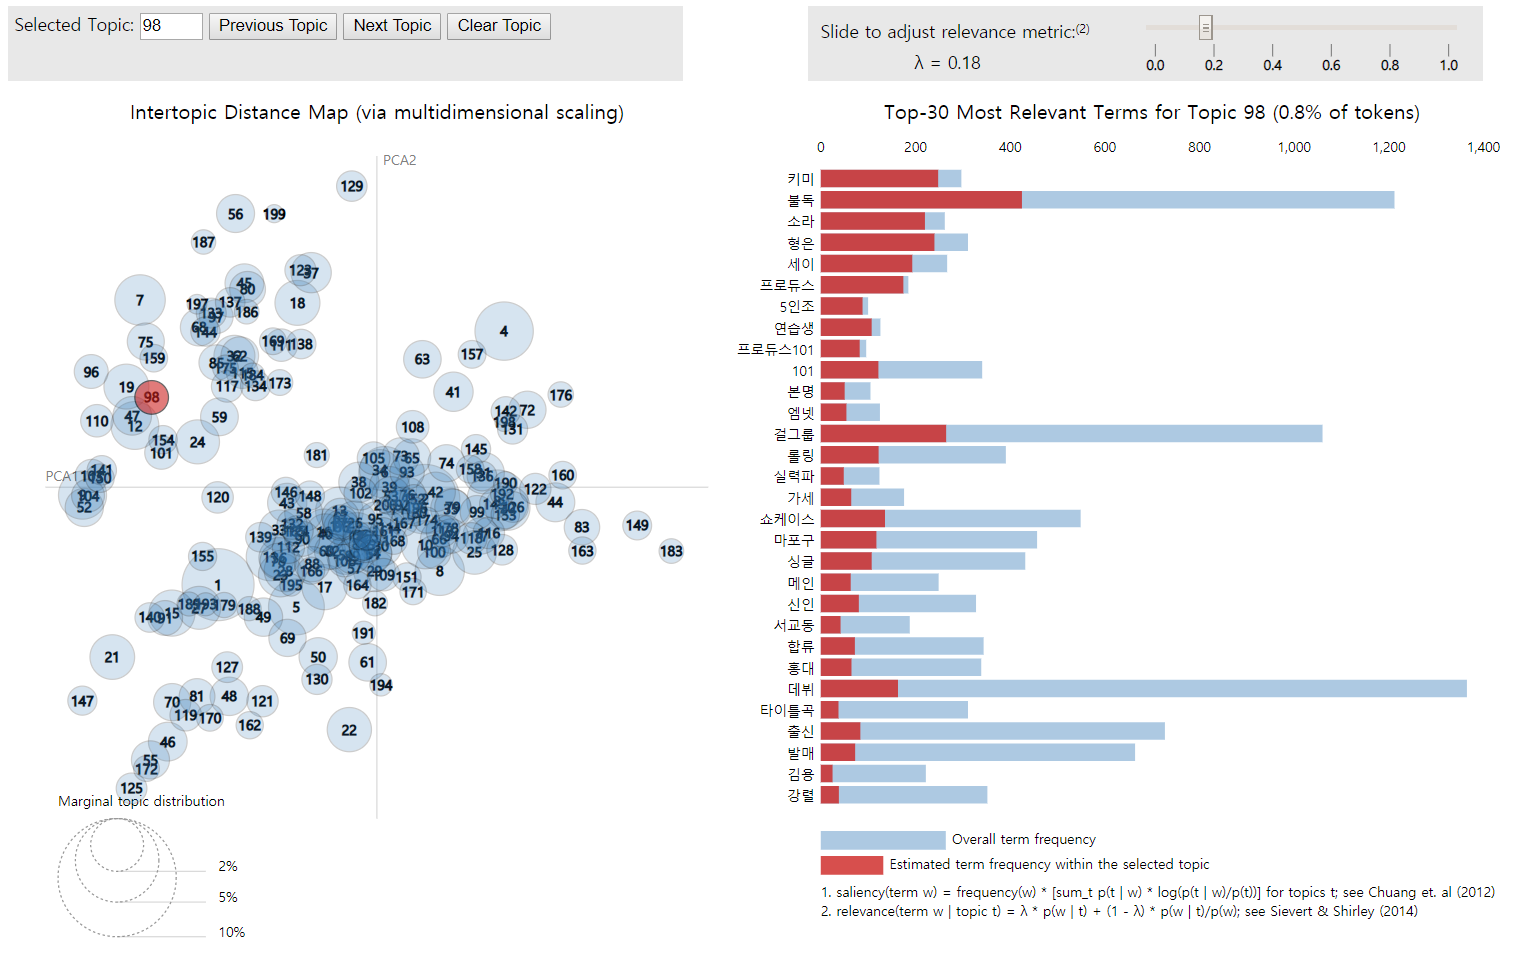
\includegraphics[keepaspectratio=true, width=0.95\linewidth]{figures/kmeans_visualization.png}
\label{fig:kmeans_ldavis}
\caption{LDAvis 를 이용한 spherical k-means 학습 결과 시각화 예시}
\end{figure}


%%%%%%%%%%%%%%%%%%%%%%%%%%%%%%%%%%%%%%%%%%%%%%%%%
\subsection{결론}

이 장에서는 문서 집합이 다양한 주제의 문서들로 구성된 경우, 문서 군집화 기법을 이용하여 단일한 주제의 문서들로 군집을 구성한 뒤 각 군집의 키워드를 추출함으로써 문서 집합을 요약하는 방법을 제안하였다.
문서 집합의 크기가 클 경우에도 효율적인 spherical k-means 학습이 가능하도록 초기화 함수를 개선하였으며, 추가적인 키워드 추출 모델의 학습 없이 군집 중심값만을 이용하여 각 군집의 키워드를 추출하는 방법도 함께 제안하였다.
제안된 방법은 7 개의 데이터를 이용한 실험을 통하여 군집화 품질의 손실없이 효율적으로 문서 군집화 학습이 가능함이 확인되었으며, 데이터의 크기가 클수록 효율성이 증가하였다.
제안된 군집 별 키워드 추출 방법은 각 군집의 의미를 해석할 수 있는 단어들을 키워드로 제공함을 정성 평가를 통하여 확인하였다.
또한 토픽 모델링의 시각화 방법인 LDAvis 를 이용하면 spherical k-mean 의 학습 결과도 시각화 할 수 있었다.

\ref{summarize_single_topic} 장에서 제안된 핵심 문장 추출 방법은 문서 집합과 키워드 집합이 주어질 경우 핵심 문장의 추출이 가능하다.
\ref{improved_kmeans} 장에서는 제안된 방법은 각 군집 별 키워드를 제공하기 때문에 \ref{summarize_single_topic} 장의 방법을 함께 이용할 경우 군집 별 핵심 문장 추출도 가능하다.

제안된 방법은 k-means 알고리즘의 한계점을 개선할 경우 더 정확한 문서 요약이 가능하다.
첫째로 k-means 알고리즘은 적절한 군집의 개수 $k$ 를 사용자가 직접 설정해야 한다.
군집의 개수가 지나치게 작으면 여러 주제가 하나의 군집으로 합쳐져 한 군집의 키워드를 해석하기 어려우며, 군집의 개수가 지나치게 클 경우 한 주제가 여러 개의 중복된 군집으로 나뉘어지기 때문에 식 \ref{eq:proposed_labeler} 이 잘 정의되지 않는다.
Silhouette 점수는 군집의 개수를 결정하는데 이용할 수 있는 척도이지만 고차원 벡터 공간에서는 잘 작동하지 않는다 \citep{almeida2011there}.
또한 Silhouette 점수는 수학적인 척도일 뿐, 사람이 느끼는 군집화 품질을 잘 반영하지는 못한다 \citep{newman2010evaluating}.
그렇기 때문에 문서 군집화 과정에서 적절한 군집의 개수를 정의할 수 있는 새로운 방법이 연구되어야 한다.

둘째로 k-means 알고리즘은 클래스의 크기가 서로 다르거나 각 클래스 별 문서의 개수가 다르더라도 각 군집의 크기가 비슷해지는 uniform effect \citep{xiong2008k} 가 발생하며, 이로 인하여 크기가 작은 클래스가 독립된 군집으로 학습이 되지 않는 문제가 존재한다.
이들은 다른 군집에 아웃라이어로 포함되는데, 제안된 키워드 추출 방법은 군집을 구분할 수 있는 단어를 키워드로 선택하기 때문에 크기가 작은 클래스로부터 추출된 단어에 의하여 잘못된 문서 요약 결과가 제공될 수 있다.
이를 해결하기 위해서는 클래스의 크기와 문서 개수에 영향을 적게 받는 문서 군집화 방법이 연구되어야 한다.

%%%%%%%%%%%%%%%%%%%%%%%%%%%%%%%%%%%%%%%%%%%%%%%%%%%%%%%%%%%%%%%%%%%%%%%%%%%%%%%
\newpage
\section{결론} \label{conclusion}

\vspace{3cm}

%%%%%%%%%%%%%%%%%%%%%%%%%%%%%%%%%%%%%%%%%%%%%%%%%%%%%%%%%%%%%%%%%%%%%%%%%%%%%%%
\newpage
\bibliography{reference}

\end{document}
